\documentclass[12pt,a4paper,oneside]{report}
\usepackage[utf8]{inputenc} 
\usepackage{babel}
\usepackage{fancyheadings}  
\usepackage[utf8]{vietnam} 
\usepackage[top=0.70in, bottom=0.70in, left=0.8in,right=0.80in]{geometry} 
\usepackage[pdftex]{graphicx} 
\usepackage{url}
\usepackage{listings}
\usepackage{multirow}
\usepackage{color}
\usepackage{titletoc}
\usepackage{array}
\usepackage{longtable}
\usepackage{fancyhdr}
\usepackage{tabulary}
\usepackage{float}
\usepackage{indentfirst} 
\usepackage{mathptmx}
\usepackage{tabu}
\usepackage{caption}
\usepackage{lscape}
\usepackage{pifont}
\usepackage{enumitem}
\usepackage{lmodern}


% Long Table Padding
\tabulinesep=3pt
% Caption Table Position
\captionsetup[tabu]{position=below}
% CONFIG DEPTH TABLE
\setcounter{tocdepth}{2} 
\setcounter{secnumdepth}{3}

% VARIABLE
\newcommand{\quotes}[1]{``#1''}
\newcommand{\single}[1]{`#1'}

% HEADER | FOOTER
\pagestyle{fancy}
\fancyhf{}
\fancyhead[RE,LO]{\leftmark}
\fancyhead[LE,RO]{\rightmark}
\fancyfoot[CE,CO]{Website live streaming}
\fancyfoot[LE,RO]{\thepage}

\renewcommand{\headrulewidth}{0.5pt}
\renewcommand{\footrulewidth}{0.5pt}

% BEGIN 
\begin{document}

\begin{titlepage}
\begin{center}
	\huge{TRƯỜNG CAO ĐẲNG THỰC HÀNH FPT} \\[10pt]
	\large{-----------------------------------------------------} \\ [10pt]
	\vspace{0.5cm}
	
\includegraphics[scale=1]{{./imgs/fpt.png}}
\end{center}

\vspace{1cm}

\begin{center}
	\textbf{{\Huge BÁO CÁO DỰ ÁN TỐT NGHIỆP}}\\
	\LARGE{Ngành Ứng Dụng Phần Mềm}\\
	\vspace{1cm}
	\rule{\textwidth}{0.5pt} \\[10pt]
	\textbf{\huge{WEBSITE LIVE STREAMING}}\\ 
	\rule{\textwidth}{0.5pt}
\end{center}

\vspace{1cm}

\begin{table}[h]
\Large
\begin{tabular}{rrl}
\hspace{3 cm} & \textbf{GVHD:} &\textbf{Thầy Nguyễn Nghiệm}\\
& \textbf{LỚP:} & \textbf{UD15201}\\
& SV: & Nguyễn Lê Tiến Bảo - PS11095\\
& & Mai Kỷ Viễn - PS10996 \\
& & Nguyễn Minh Khôi - PS11136\\
& & Nguyễn Trường An - PS10672 \\
\end{tabular}
\end{table}

\vspace{3cm}

\begin{center}
{\footnotesize \Large\today}
\end{center}
\end{titlepage}

 \tableofcontents
 \chapter{MỞ ĐẦU}
\section{Giới Thiệu}
\subsection{Lý do chọn đề tài}
Từ 1997, Internet chính thức được cung cấp rộng rãi, là ngày đầu Việt Nam được hoà vào mạng toàn cầu, dẫn đến phát triển bùng nổ của Internet với tốc độ đường truyền cao. Hình thành nên nhiều dịch vụ thông qua internet như game online (Liên Minh Huyền Thoại), mạng xã hội (Facebook, Youtube…).
\par Theo thống kê, Việt Nam hiện đang có khoản 70\% dân số đang sử dụng internet, đồng thời có 68,17 triệu người đang dùng các dịch vụ trên internet. Trong khi đó Viêt Nam ta có 145,8 triệu kết nối di động trong năm 2020, vậy có thể nói rằng các ngành dịch vụ phát triển trên internet của Việt Nam hiện và đang rất thu hút và phát triển đặc biệt là giới trẻ Việt Nam.
\par Năm 2020, đại dịch lây nhiễm \textbf{Covid-19} bùng nổ và trở thành như đại dịch toàn cầu. Từ đó đến nay (01-05-2021), đã qua một năm nhưng tình trạng vẫn diễn ra theo hướng xấu đi. Để giảm các tình trạng lây lan, nhà nước buộc phải áp dụng cái biện pháp giãn cách, buộc người dân ở nhà theo các chỉ thị. Nắm bắt được tình hình này, nhóm đã tận dụng tối đa tiềm lực và các xu hướng phát triển các dịch vụ trên Internet. Qua đó nhóm sẽ tạo ra một ứng dụng có thể sử dụng một cách phổ biến cho cộng đồng với mọi lứa tuổi tham gia. Sản phảm có thể giúp chia sẽ các kiến thức, sở thích cá nhân, du lịch, khám phá, thể thao, tin tức xã hội qua hình thức \textbf{trực tuyến}. Phát triển theo quy luật cung và cầu. Do đó đề tài được chọn là một ứng dụng có thể giúp người dùng có thể chia sẻ các nội dung một cách trực tiếp thông qua nền tảng \textbf{Website}. 

\subsection{Ý tưởng của đề tài}
Website streaming là dự án cho phép người dùng chia sẻ trực tiếp nội dung qua video, có thể tương tác trực tiếp qua lại, đồng thời có khả năng mở rộng và khả năng tương thích cao. Bên cạnh đó ứng dụng sẽ tích hợp thêm ví tiền online giúp người dùng nhận và gửi một khoản chi phí cho các chuyên đề mang tính từ thiện, giáo dục hay gây quỹ cho cộng đồng thông qua một phần mềm liên kết trung gian.
\subsection{Mục tiêu của dự án}
 \begin{itemize}
       \item Tìm hiểu về WebRTC (Web Real Time Communication)
        \item Nắm bắt về cách thức xây dựng phần mềm trên nền tảng website
        \item Phân tích thiết kế kiến trúc của phần mềm
        \item Xây dựng phần mềm
       \end{itemize}

\section{Ban Thành Viên Dự Án}
\begin{center}
\begin{longtabu} to \textwidth {| m{5cm} | m{10cm} |}
    \hline
    \multicolumn{1}{|c|}{Thành viên} & \multicolumn{1}{|c|}{Nhiệm vụ}  \\ \hline
    % BAO
      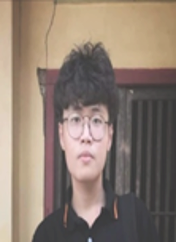
\includegraphics[width=\linewidth, height=50mm]{{./imgs/bao.png}}
    &
      \begin{itemize}
        \item{\textbf{Nguyễn Lê Tiến Bảo}}
        \item Quản lý dự án
        \item Xây dựng bản đặc tả yêu cầu (Streamer, Viewer)
        \item Phân tích thiết kế \& chọn loại công nghệ áp dụng
        \item Xử lý và hoàn thiện cái chức năng chính \& logic cho sản phẩm
        \item Hoàn thiện báo cáo
        \item Đánh giá cá nhân, nhóm trong suốt quá trình làm việc
      \end{itemize}
    \\ \hline
    % VIEN
      
\includegraphics[width=\linewidth, height=50mm]{{./imgs/vien.png}}
    &
      \begin{itemize}
       \item{\textbf{Mai Kỷ Viễn}}
       \item Thiết kế vẽ Use Case (Streamer, Viewer, Model)
        \item Thiết kế vẽ mô hình ERD
       \item Xây dựng chức năng tìm kiếm \& công cụ thống kê
        \item Chức năng chỉnh sửa video
        \item Hỗ trợ làm Document
       \end{itemize}
    \\ \hline
     % KHOI
      
\includegraphics[width=\linewidth, height=50mm]{{./imgs/khoi.png}}
    &
      \begin{itemize}
       \item{\textbf{Nguyễn Minh Khôi}}
       \item Thiết kế vẽ Mockup 
       \item Phát triển giao diện và các chức năng live stream
       \item Phát triển các chức năng tương tác (Chat, Like, Subscribe, Donate)
       \item Chức năng block spam chat
       \item Kiểm thử sản phẩm
      \end{itemize}
    \\ \hline
     % AN
      
\includegraphics[width=\linewidth, height=50mm]{{./imgs/an.png}}
    &
      \begin{itemize}
       \item{\textbf{Nguyễn Trường An}}
      	\item Thiết kế vẽ các Mockup
        \item Phát triển phần giao diện (Xác thực, Donate, Hồ sơ, Lịch sử)
        \item Viết các test case (Các chức năng video, đăng nhập, thống kê,...)
        \item Kiểm thử sản phẩm
      \end{itemize}
    \\ \hline
\end{longtabu}
\end{center}




 \chapter{KHẢO SÁT}
\section{Yêu Cầu Của Khách Hàng}
\textbf{Website Live Streaming} là ứng dụng nhằm đắp ứng nhu cầu trao giao tiếp, kết bạn và trao đổi thông tin bằng văn bản hay các video theo từng đề tài thông qua một số \textbf{channel} nên sẽ được chia làm hai phần chính gồm.
 \begin{itemize}
 	\item \textbf{Streamer}: Người phát sóng trực tiếp chia sẻ nội dung cho người xem.
	\item \textbf{Viewer}: Người xem những nội dung đã và đang chia sẻ từ Streamer. Có thể tương tác trực tiếp tới streamer qua các hình thức \textbf{like,comment,donate}.
 \end{itemize}

\section{Các Chức Năng Cho Hệ Thống}
\begin{itemize}
	\item Xác thực người dùng
 		\begin{itemize}
   			 \item Đăng ký tài khoản.
			 \item Đổi mật khẩu.
   			 \item Đăng nhập/đăng xuất.
 		 \end{itemize}
	 \item Quản lý tài khoản và channel
 		\begin{itemize}
   			 \item Chỉnh sửa thông tin cá nhân của tài khoản, có thể chuyển đổi vai trò, dùng \textbf{visa} để thanh toán.
   			 \item Mỗi tài khoản với vai trò streamer sẽ được cấp một mã phòng cố định dựa theo \textbf{nickname} (nickname có thể tuỳ biến) để có thể livestream. Trước khi bắt đầu phát sóng, streamer sẽ tự chọn hashtag, đặt tiêu đề và viết mô tả cho video của mình. Khi bắt đầu livestream, hệ thống sẽ tự gửi mail cho các tài khoản đã theo dõi kênh.
			 \item Theo dõi channel: mỗi tài khoản có thể đăng ký kênh mà họ yêu thích và được thông báo.
			\item Quy đổi xèng sang tiền.
			\item Tìm kiếm các video đang phát sóng theo chủ đề/tên tài khoản/ngày tháng.
 	 	\end{itemize}
	\item Tương tác trong quá trình phát sóng
		\begin{itemize}
			\item Thích.
			\item Bình luận.
			\item Donate.
		\end{itemize}
	\item Đề xuất cho các chức năng
		\begin{itemize}
			\item Mỗi tài khoản có thể tạo nhiều kênh cho phòng livestream. Có thể spam bất kỳ tài khoản.
			\item Thông báo livestream của kênh thông qua tin nhắn thông báo, email.
			\item Đề xuất các video, channel đang đứng top và có nhiều lượt xem.
		\end{itemize}
\end{itemize}

\section{Lập kế hoạch dự án}

 \begin{center}
\begin{longtabu} to \textwidth {| m{1cm} | m{3cm} | m{2cm} | m{2cm} | m{3cm} | m{3cm} | m{1cm} |}
\hline STT & \textbf{Công việc} & \textbf{Bắt đầu} & \textbf{Kết thúc} & \textbf{Thành viên} & \textbf{Tình trạng} & \textbf{Ghi chú}\\ \hline
\endfirsthead
\hline \textbf{STT} & \textbf{Công việc} & \textbf{Bắt đầu} & \textbf{Kết thúc} & \textbf{Thành viên} & \textbf{Tình trạng} & \textbf{Ghi chú}\\ \hline
\endhead
\hline
\endfoot
\multicolumn{1}{|c|}{\textbf{1}} & \multicolumn{5}{|c|}{\textbf{Phân tích yêu cầu khách hàng}} &   
\\ \hline
\multicolumn{1}{|c|}{1.1} & Xây dựng bản đặc tả hệ thống & 05/05/2021 & 05/05/2021 & Cả nhóm & Đã hoàn thành &  
\\ \hline
\multicolumn{1}{|c|}{1.2} & Vẽ use case & 05/05/2021 & 05/05/2021 & Viễn & Đã hoàn thành &  
\\ \hline
\multicolumn{1}{|c|}{1.3} & Vẽ sơ đồ tổng quan   & 05/05/2021 & 05/05/2021 & Viễn & Đã hoàn thành &  
\\ \hline
\multicolumn{1}{|c|}{\textbf{2}} & \multicolumn{5}{|c|}{\textbf{Thiết kế hệ thống}} &  
\\ \hline
\multicolumn{1}{|c|}{2.1} & Phát thảo mô hình công nghệ ứng dụng & 05/05/2021 & 05/05/2021 & Cả nhóm & Đã hoàn thành &  
\\ \hline
\multicolumn{1}{|c|}{2.2} & Phát thảo layout & 05/05/2021 & 05/05/2021 &  An & Đã hoàn thành &  
\\ \hline
\multicolumn{1}{|c|}{2.3} & Phái thảo giao diện các chức năng & 05/05/2021 & 05/05/2021 & An & Đã hoàn thành &    
\\ \hline
\multicolumn{1}{|c|}{2.4} & Thiết kế sơ đồ quan hệ thực thể (ERD) & 05/05/2021 & 05/05/2021 & Viễn & Đã hoàn thành &  
\\ \hline
\multicolumn{1}{|c|}{2.5} & Thiết kế các chi tiết thực thể & 05/05/2021 & 05/05/2021 & Bảo, Khôi, Viễn  & Đã hoàn thành &  
\\ \hline
\multicolumn{1}{|c|}{\textbf{3}} & \multicolumn{5}{|c|}{\textbf{Thực hiện dự án}} &   
\\ \hline
\multicolumn{1}{|c|}{3.1} & Thiết kế cơ sở dữ liệu & 05/05/2021 & 05/05/2021 & Cả nhóm & Đã hoàn thành &  
\\ \hline
\multicolumn{1}{|c|}{3.2} & Thiết kế giao diện & 05/05/2021 & 05/05/2021 & Cả nhóm & Đã hoàn thành &  
\\ \hline
\multicolumn{1}{|c|}{3.3} & Xây dựng các thư viện tiện ích& 05/05/2021 & 05/05/2021 & Cả nhóm & Đã hoàn thành &  
\\ \hline
\multicolumn{1}{|c|}{3.4} & Viết các store procedure & 05/05/2021 & 05/05/2021 & Cả nhóm & Đã hoàn thành &  
\\ \hline
\multicolumn{1}{|c|}{3.5} & Lập trình các chức năng nghiệp vụ & 05/05/2021 & 05/05/2021 & Cả nhóm & Đã hoàn thành &  
\\ \hline
\multicolumn{1}{|c|}{3.5} & Xây dựng các chức năng cho live stream + tương tác & 05/05/2021 & 05/05/2021 & Bảo, Khôi & Đã hoàn thành &  
\\ \hline
\multicolumn{1}{|c|}{3.6} & Xây dựng trang thống kê & 05/05/2021 & 05/05/2021 & Bảo, Viễn & Đã hoàn thành &  
\\ \hline
\multicolumn{1}{|c|}{\textbf{4}} & \multicolumn{5}{|c|}{\textbf{Kiểm thử}} &   
\\ \hline
\multicolumn{1}{|c|}{4.1} & Xây dựng kịch bản kiểm thử & 05/05/2021 & 05/05/2021 & Khôi, An & Đã hoàn thành &  
\\ \hline
\multicolumn{1}{|c|}{4.2} & Thực hiện kiểm thử & 05/05/2021 & 05/05/2021 & Khôi, An & Đã hoàn thành &  
\\ \hline
\multicolumn{1}{|c|}{\textbf{5}} & \multicolumn{5}{|c|}{\textbf{Đóng gói sản phẩm}} &   
\\ \hline
\multicolumn{1}{|c|}{5.1} & Đóng gói sản phẩm & 05/05/2021 & 05/05/2021 & Bảo & Đã hoàn thành &  
\\ \hline
\multicolumn{1}{|c|}{5.2} & Viết tài liệu hướng dẫn sử dụng & 05/05/2021 & 05/05/2021 & Bảo & Đã hoàn thành &  
\end{longtabu} 
\end{center}




 \chapter{PHÂN TÍCH}
\section{Mô Hình}

\subsection{Mô hình triển khai hệ thống}
	\begin{center}
	\begin{figure}[H]
		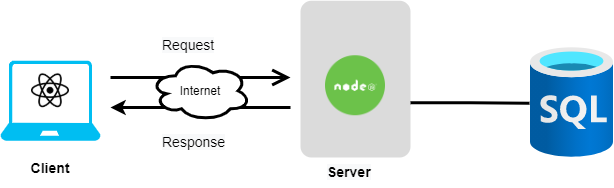
\includegraphics[width=17cm]{{./imgs/implement_tech_diagram}}
		\caption{Mô hình triển khai}
	\end{figure}
	\end{center}
	
\subsection{Mô tả sơ đồ}
\begin{center}
\begin{longtabu} to \textwidth {| m{5cm} | m{5cm} | m{5cm} |}
\caption{Mô tả sơ đồ} \\
\hline \textbf{Tên} & \textbf{Mô tả} & \textbf{Công nghệ} \\ \hline
\endfirsthead
\hline \textbf{Tên} & \textbf{Mô tả} & \textbf{Công nghệ} \\ \hline
\endhead
\hline
\endfoot
Client & Là nơi User tương tác gửi các yêu cầu, các chức năng và dữ liệu đến máy chủ để máy chủ xử lý yêu cầu và trả về kết quả & ReactJS
\\ \hline
Server & Là chấp nhận tất cả yêu cầu hợp lệ từ Client, sau đó trả về kết quả đã tính toán & NodeJS
\\ \hline
Database & Là nơi lưu trữ dữ liệu & MySQL
\\ \hline
Request, Response & Gửi và nhận dữ liệu thông qua Internet & Giao thức: TCP/IP, HTTP Protocol
\\ \hline
\end{longtabu}
\end{center}

\section{Sơ Đồ Use Case}
\subsection{Tổng quan}
	\begin{center}
		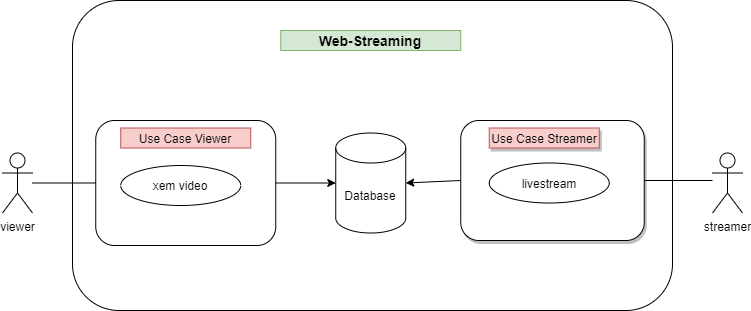
\includegraphics[width=17cm]{{./imgs/usecase_model.png}}
	\end{center}

\subsection{Use case cho viewer}
	\begin{center}
		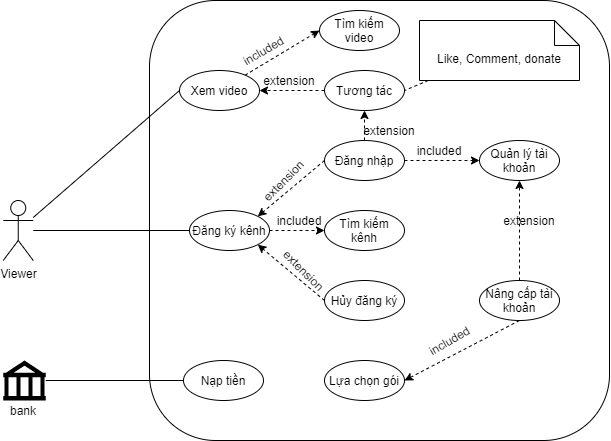
\includegraphics[width=17cm]{{./imgs/usecase_viewer.png}}
	\end{center}
	
\subsection{Use case cho streamer}
	\begin{center}
		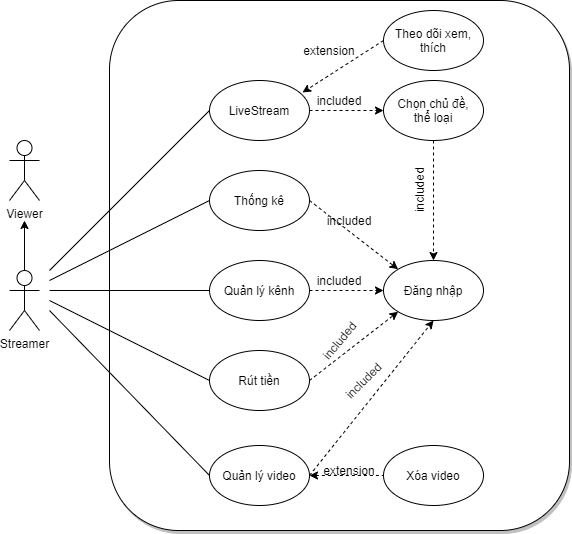
\includegraphics[width=17cm]{{./imgs/usecase_streamer.png}}
	\end{center}
		
	
\section{Đặc Tả Hệ Thống}
\subsection{Chi tiết dành cho Viewer}

 \begin{center}
\begin{longtabu} to \textwidth {| m{5cm} | m{5cm} | m{5cm} |}
\caption{Mô tả chi tiết Use Case Viewer}  \\ 
\hline \textbf{Tên chức năng} & \textbf{Mô tả} & \textbf{Ghi chú} \\ \hline
\endfirsthead
\hline \textbf{Tên chức năng} & \textbf{Mô tả} & \textbf{Ghi chú} \\ \hline
\endhead
\hline
\endfoot
Đăng ký & Người dùng đăng ký tài khoản để truy cập vào hệ thống  &
\\ \hline
Đăng nhập/Đăng xuất &  Bước đầu tiến khi vào một ứng dụng và thoát ứng dụng & 
\\ \hline
Menu & Danh sách các video, kênh và tài khoản được đưa ra tuy theo sở thích, lượt xem cho người dùng & Có thể tự động \quotes{play} theo kênh đề xuất
\\ \hline
Quản lý tài khoản & Thêm, cập nhật thông tin cá nhân của tài khoản & 
\\ \hline
Nâng cấp tài khoản & Mua các gói trả phí & 
\\ \hline
Chuyển đổi tiền tệ & Giúp người dùng nạp và rút tiền từ tài khoản vào thẻ ngân hàng & Có thể liên kết gián tiếp qua các ứng dụng thanh toán trực tuyến (ZaloPay, Momo,\dots)
\\ \hline
Kênh đăng ký & Danh sách những kênh yêu thích & Nhận được thông báo khi kênh đăng hoạt động 
\end{longtabu} 
\end{center}
   
\subsection{Chi tiết dành cho Streamer}
\begin{center}
\begin{longtabu} to \textwidth {| m{5cm} | m{5cm} | m{5cm} |}
\caption{Mô tả chi tiết Use Case Streamer} \\
\hline \textbf{Tên chức năng} & \textbf{Mô tả} & \textbf{Ghi chú} \\ \hline
\endfirsthead
\hline \textbf{Tên chức năng} & \textbf{Mô tả} & \textbf{Ghi chú} \\ \hline
\endhead
\hline
\endfoot
Đăng nhập/Đăng xuất &  Bước đầu tiến khi vào một ứng dụng và thoát ứng dụng  &
\\ \hline
Live Stream &  Nơi mà streamer dùng để tạo các video và chia sẻ trưc tuyến tới người xem & Mỗi tài khoản được cấp cho một mã phòng nhất định
\\ \hline
Quản lý kênh & Nơi lưu trữ dữ liệu chính của hệ thống & Có thể sử dụng nhiều hệ cơ sở dữ liệu khác nhau (SQL Server, MySQL, MongoDB..)
Mỗi service có một hệ cơ sở dữ liệu riêng biệt
\end{longtabu}
\end{center}



\chapter{THIẾT KẾ}
\section{Mô Hình Công Nghệ}
\subsection{Tổng quan công nghệ}
\subsubsection{WebSocket}
WebSocket là một giao thức được phổ biến cho việc phát triển ứng dụng real-time, cho phép các trình duyệt giao tiếp với nhau theo thời gian thực. Giao thức WebSocket  cung cấp một cách thức để tạo những kết nối bền bỉ, độ trễ thấp để hỗ trợ giao tiếp giữa client và server (giap tiếp hai chiều - two way communication). Sử dụng WebSockets có thể tạo một ứng dụng \textbf{real-time} đúng nghĩa như ứng dụng chat, sử dụng 1 tiến trình để nói chuyện với tiến trình khác, phối hợp soạn thảo văn bản, giao dịch chứng khoán hay game online nhiều người chơi cùng lúc.
\par Một chức năng khác của socket là giúp các tầng \textbf{TCP} định danh ứng dụng mà dữ liệu sẽ được gửi tới thông qua sự ràng buộc với một cổng port (thể hiện là một con số cụ thể), từ đó tiến hành kết nối giữa client và server.

	\begin{center}
	\begin{figure}[H]
		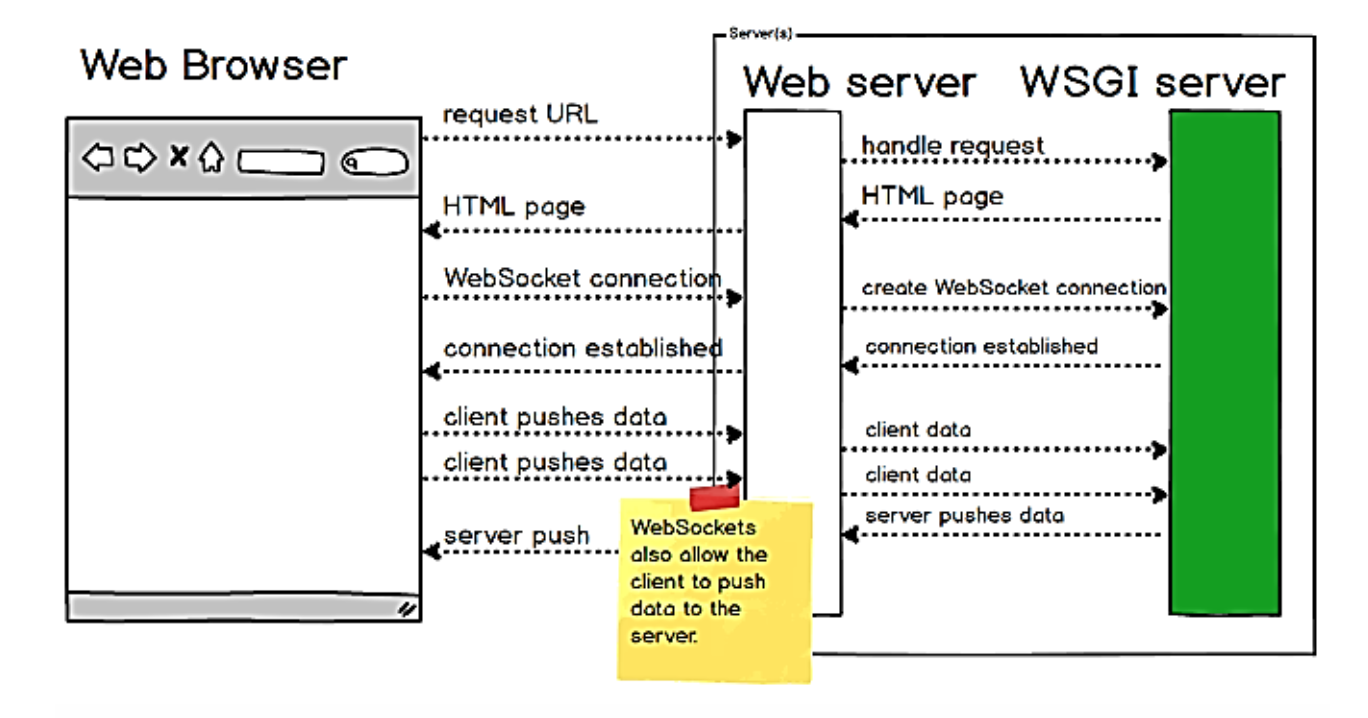
\includegraphics[width=17cm]{{./imgs/WebSocket_structure}}
		\caption{Sơ đồ hoạt động của WebSocket}
	\end{figure}
	\end{center}  
\subsubsection{Giao thức TCP/IP}
	\begin{center}
	\begin{figure}[H]
		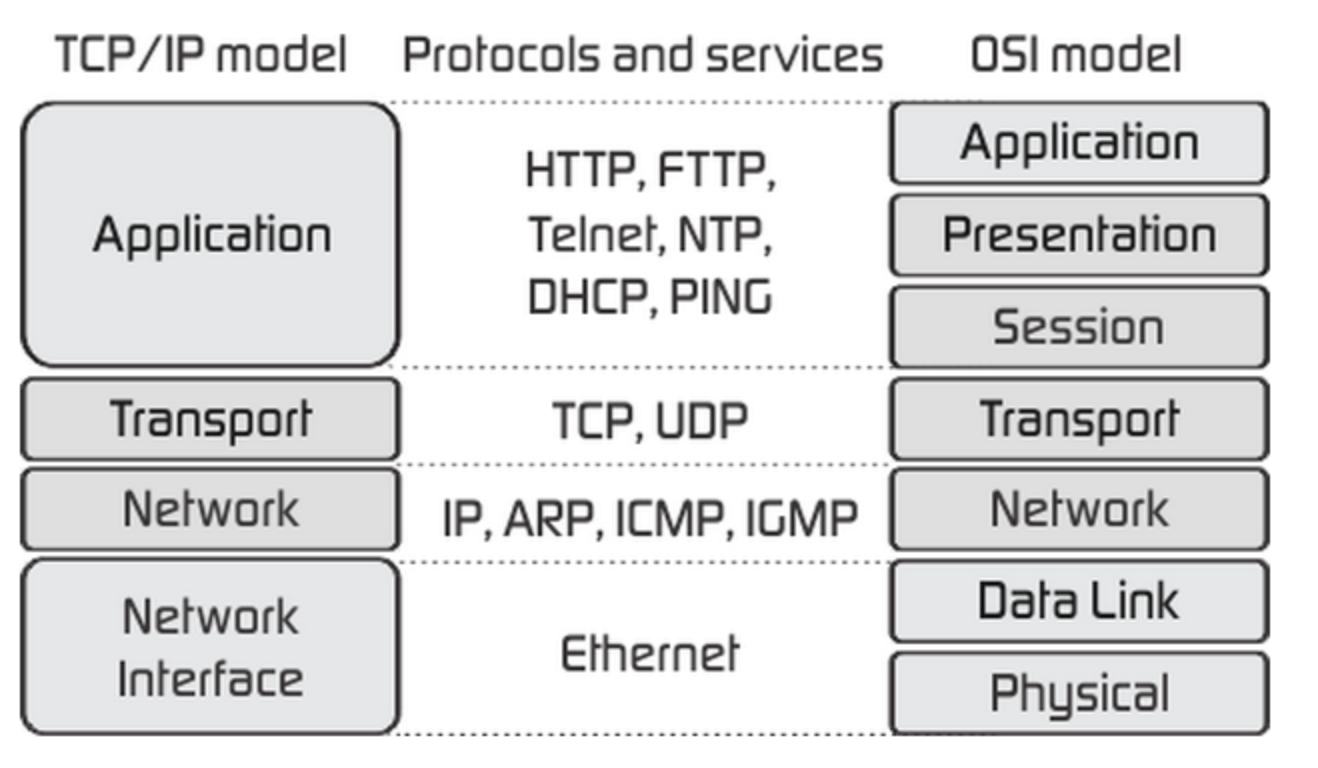
\includegraphics[width=17cm]{{./imgs/TCP_OSI}}
		\caption{TCP/IP với mô hình OSI}
	\end{figure}
	\end{center} 


\paragraph{Giao thức được chia thành các tầng mạng trong mô hình OSI}
	\begin{itemize}
       \item \textbf{Tầng Application}: Nhiệm vụ của tầng này đó là cung cấp các ứng dụng, trao đổi dữ liệu được chuẩn hóa. Trong tầng ứng dụng bao gồm nhiều giao thức cụ thể như HTTP, FTP, POP3, SMTP, SNMP. Mỗi giao thức này sẽ có chức năng và nhiệm vụ cụ thể.
        \item \textbf{Tầng Network}: Nhiệm vụ của tầng internet là xử lý các gói tin, sau đó kết nối với các mạng độc lập để vận chuyển các gói dữ liệu đã được mã hóa qua các ranh giới mạng.
        \item \textbf{Tầng Transport}: Nhiệm vụ của tầng giao vận là duy trì liên lạc đầu cuối trên toàn mạng. Tầng giao vận bao gồm giao thức \textbf{TCP và UDP}. Trong nhiều trường hợp giao thức UDP sẽ được thay thế TCP.
       \end{itemize}
      
     \begin{center}
	\begin{figure}[H]
		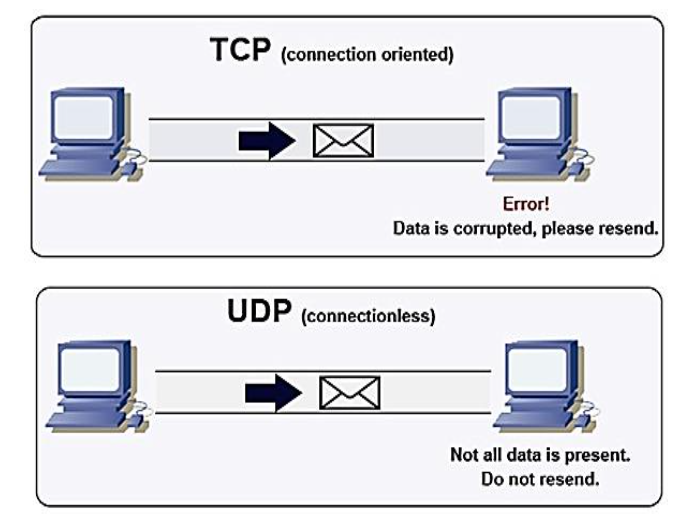
\includegraphics[width=17cm]{{./imgs/TCP_UDP_flow}}
		\caption{Cách thức truyền nhận dữ liệu}
	\end{figure}
	\end{center}  
  \par Nguyên lý hoạt động của giao thức này là sự kết hợp giữa hai giao thức riêng biệt, đó là giữa giao thức kiểm soát truyền tin và giao thức internet. Đầu tiên giao thức IP sẽ cho phép các gói tin được gửi qua mạng bằng cách cho biết những gói tin này được gửi qua đâu và làm như thế nào. \par
 Ngay sau khi được yêu cầu giao thức IP sẽ điều khiển truyền dẫn để giúp truyền những dữ liệu đáng tin cậy thông qua các kết nối mạng internet. Cuối cùng giao thức TCP sẽ kiểm tra lại các gói dữ liệu một lần nữa xem có lỗi và xảy ra vấn đề gì không. Nếu không có lỗi thì sẽ truyền đến vị trí cần thiết, trong trường hợp có lỗi thì sẽ gửi lại yêu cầu truyền lại.

\subsubsection{NodeJS}
NodeJS là một nền tảng được xây dựng trên \textbf{V8 JavaScript Engine} – trình thông dịch thực thi mã JavaScript, giúp xây dựng các ứng dụng web một cách đơn giản và dễ dàng mở rộng. \par
NodeJS được phát triển bởi Ryan Dahl vào năm 2009 và có thể chạy trên nhiều hệ điều hành khác nhau: OS X, Microsoft Windows, Linux. Các ưu điểm của NodeJS.
\begin{itemize}
       \item NodeJS được viết bằng JavaScript với cộng đồng người dùng lớn mạnh.
        \item Tốc độ xử lý nhanh. Nhờ cơ chế xử lý \textbf{bất đồng độ (non-blocking)}, NodeJS có thể xử lý hàng ngàn kết nối cùng lúc mà không gặp bất cứ khó khăn nào.
        \item Dễ dàng mở rộng.
       \end{itemize}

\subsubsection{MySQL}
MySQL là chương trình dùng để quản lý hệ thống cơ sở dữ liệu (CSDL), trong đó CSDL là một hệ thống lưu trữ thông tin. được sắp xếp rõ ràng, phân lớp ngăn nắp những thông tin mà mình lưu trữ. Các ưu điểm của MySQL.
\begin{itemize}
       \item Khả năng mở rộng và tính linh hoạt.
        \item Hiệu năng cao.
        \item Bảo vệ dữ liệu mạnh mẽ.
        \item Tính sẵn sàng cao.
        \item Mã nguồn mở tự do
       \end{itemize}

%%%%%%%%%%%%%%%%%%%%%%%%%%%%%%%%
\section{Mô Hình Triển Khai}

	\begin{center}
	\begin{figure}[H]
		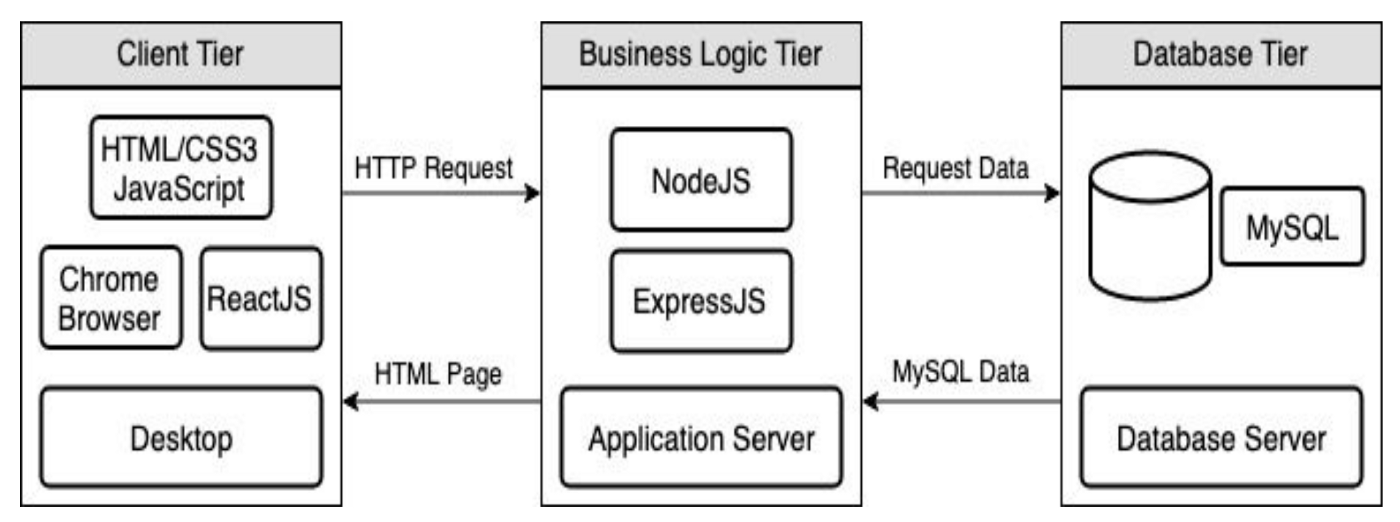
\includegraphics[width=17cm]{{./imgs/implement_diagram}}
		\caption{Mô hình triển khai công nghệ}
	\end{figure}
	\end{center}
	
	\begin{center}
	\begin{figure}[H]
		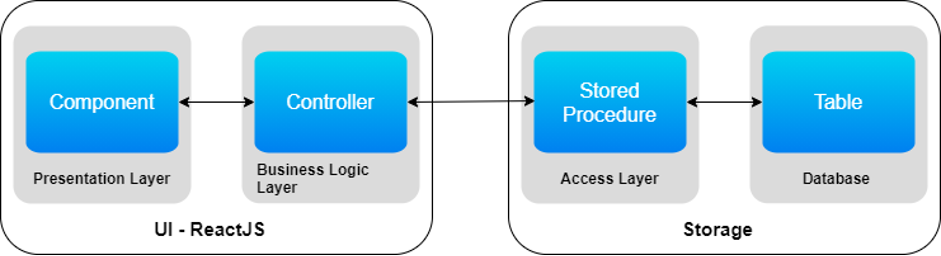
\includegraphics[width=17cm]{{./imgs/technoligy_diagram}}
		\caption{Sơ đồ luồng dữ liệu}
	\end{figure}
	\end{center}

\begin{center}
\begin{longtabu} to \textwidth {| m{5cm} | m{5cm} | m{5cm} |}
\caption{Mô tả sơ đồ} \\
\hline \textbf{Tên đối tượng} & \textbf{Mô tả} & \textbf{Yêu cầu} \\ \hline
\endfirsthead
\hline \textbf{Tên đối tượng} & \textbf{Mô tả} & \textbf{Yêu cầu} \\ \hline
\endhead
\hline
\endfoot
Client Tier & Phía giao diện sẽ được viết bằng HTML, CSS, Javascript \& thư viện ReactJS & Tương tác \& truy cập tới các tính năng của ứng dụng 
\\ \hline
Business Logic Tier & Phía Server sẽ được phát triển bằng NodeJS \& ExpressJS như 1 cầu nối giao tiếp tới giao diện và cơ sở dữ liệu & Tiếp nhận các yêu cầu HTTP được gửi từ người dùng và gửi phản hồi thích hợp
\\ \hline
Database Tier & Dùng cơ sở dữ liệu MySQL để lưu trữ & Lưu trữ tất cả dữ liệu của ứng dụng
\end{longtabu}
\end{center}
	
%%%%%%%%%%%%%%%%%%%%%%%%%5

\section{Thiết Kế Giao Diện}
\subsection{Sitemap}
	\begin{center}
		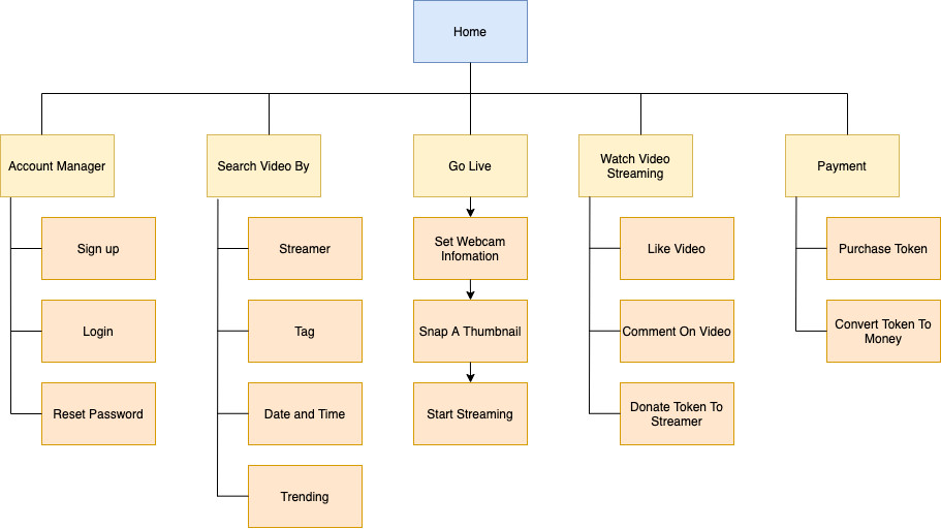
\includegraphics[scale=1]{{./imgs/sitemap.png}}
	\end{center}

\begin{center}
\begin{longtabu} to \textwidth {| m{4cm} | m{5cm} | m{6cm} |}
\caption{Mô tả sitemap}  \\ 
\hline
\multicolumn{1}{|c|}{\textbf{Tên}}              & \multicolumn{1}{c|}{\textbf{Chức năng}} & \multicolumn{1}{c|}{\textbf{Mô tả}} \\ \hline
\multirow{3}{*}{Account manager}       & Sign up                        & Đăng ký tài khoản          \\ \cline{2-3} 
                                       & Login                          & Đăng nhập vào hệ thống     \\ \cline{2-3} 
                                       & Reset password                 & Đổi mật khẩu               \\ \hline
\multirow{4}{*}{Search video}          & Streamer                       & Tìm kiếm theo streamer     \\ \cline{2-3} 
                                       & Tag                            & Tìm kiếm theo tag          \\ \cline{2-3} 
                                       & Date and time                  & Tìm kiếm theo thời gian    \\ \cline{2-3} 
                                       & Trending                       & Tìm kiếm theo thịnh hành   \\ \hline
\multirow{3}{*}{Go live}               & Set webcam information         & Thiết lập thông tin video  \\ \cline{2-3} 
                                       & Snap a thumbnail               & Chụp thumbnail cho video   \\ \cline{2-3} 
                                       & Start streaming                & Bắt đầu stream             \\ \hline
\multirow{3}{*}{Watch video streaming} & Like video                     & Thích video                \\ \cline{2-3} 
                                       & Comment on video               & Viết bình luận cho video   \\ \cline{2-3} 
                                       & Donate token to streamer       & Tặng token cho streamer    \\ \hline
\multirow{2}{*}{Payment}               & Purchase token                 & Mua token                  \\ \cline{2-3} 
                                       & Convert                        & Quy đổi token              \\ \hline
\end{longtabu}
\end{center}
	
\subsection{Giao diện chức năng}
	\begin{center}
	\begin{figure}[H]
		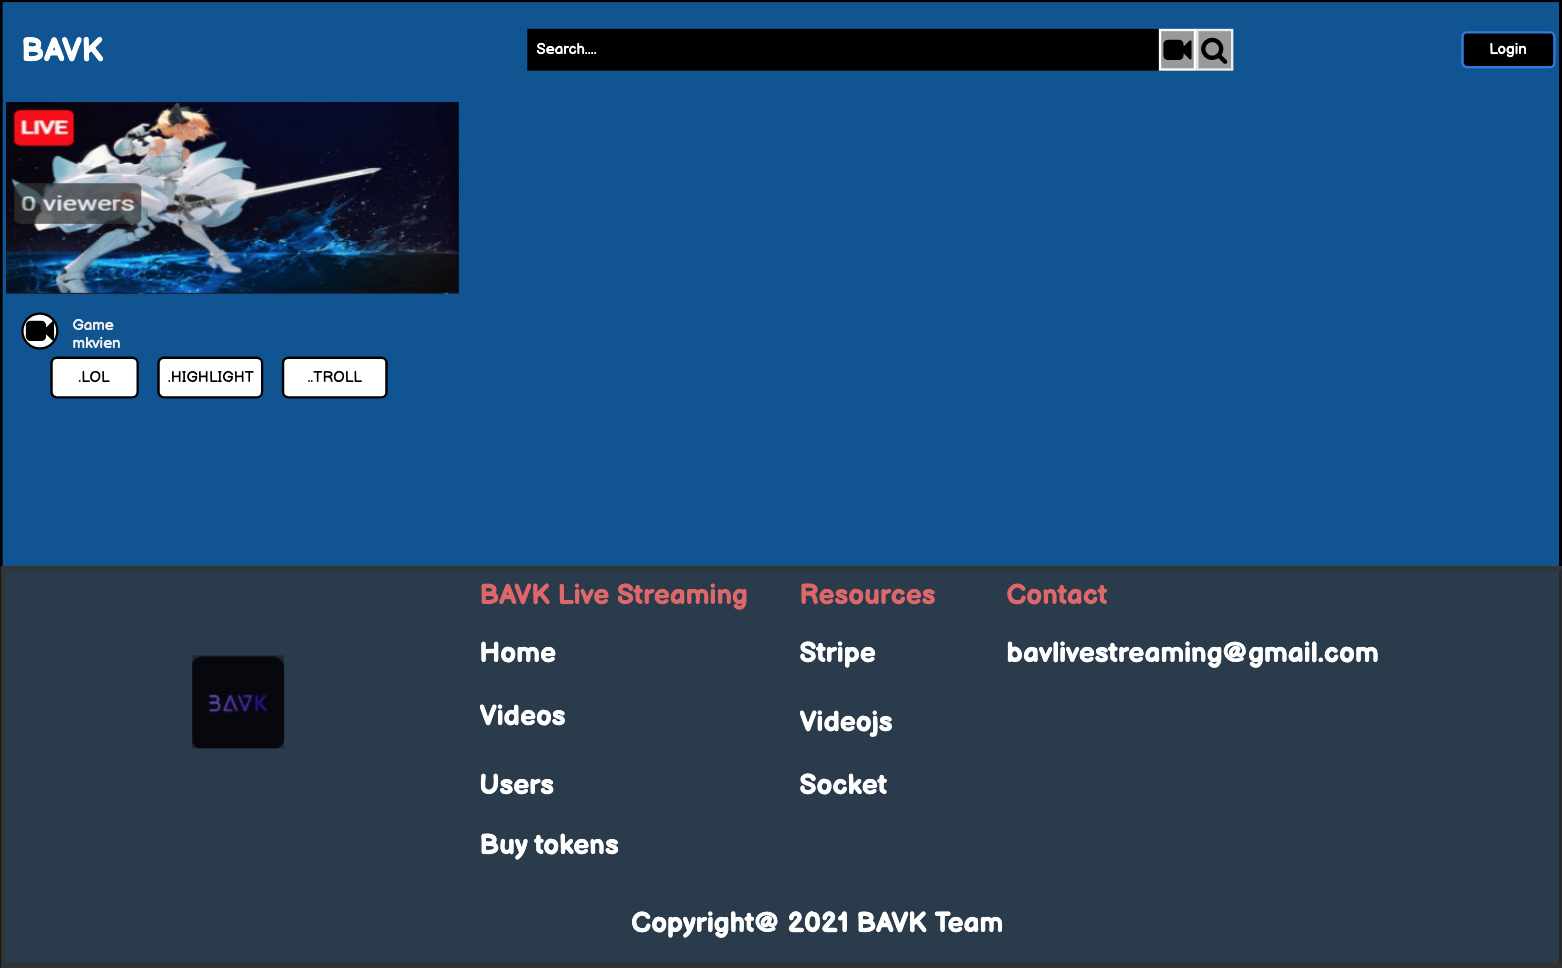
\includegraphics[width=17cm]{{./imgs/landing_page}}
		\caption{Trang chủ}
	\end{figure}
	\end{center}
	
\begin{center}
\begin{longtabu} to \textwidth {| m{1cm} | m{4cm} | m{3cm} | m{7cm} |}
\caption{Mô tả trang chủ} \\
    \hline \textbf{STT}  & \textbf{Điều khiển} & \textbf{Sự kiện} & \textbf{Mô tả} \\ \hline
    \endfirsthead
    \hline \textbf{STT}  & \textbf{Điều khiển} & \textbf{Sự kiện} & \textbf{Mô tả} \\ \hline
    \endhead
      1 & Search bar  & Input & Tìm kiếm tương đối các thông tin liên quan từ khóa người dùng nhập vào \\
      \hline
      2 & Video list & Initialize & Hiển thị các video đang được streaming  \\
      \hline
      3 & Footer  & Initialize & Chứa các thông tin chung, bản quyền của website \\
      \hline
\end{longtabu}
\end{center}
	
	\begin{center}
	\begin{figure}[H]
		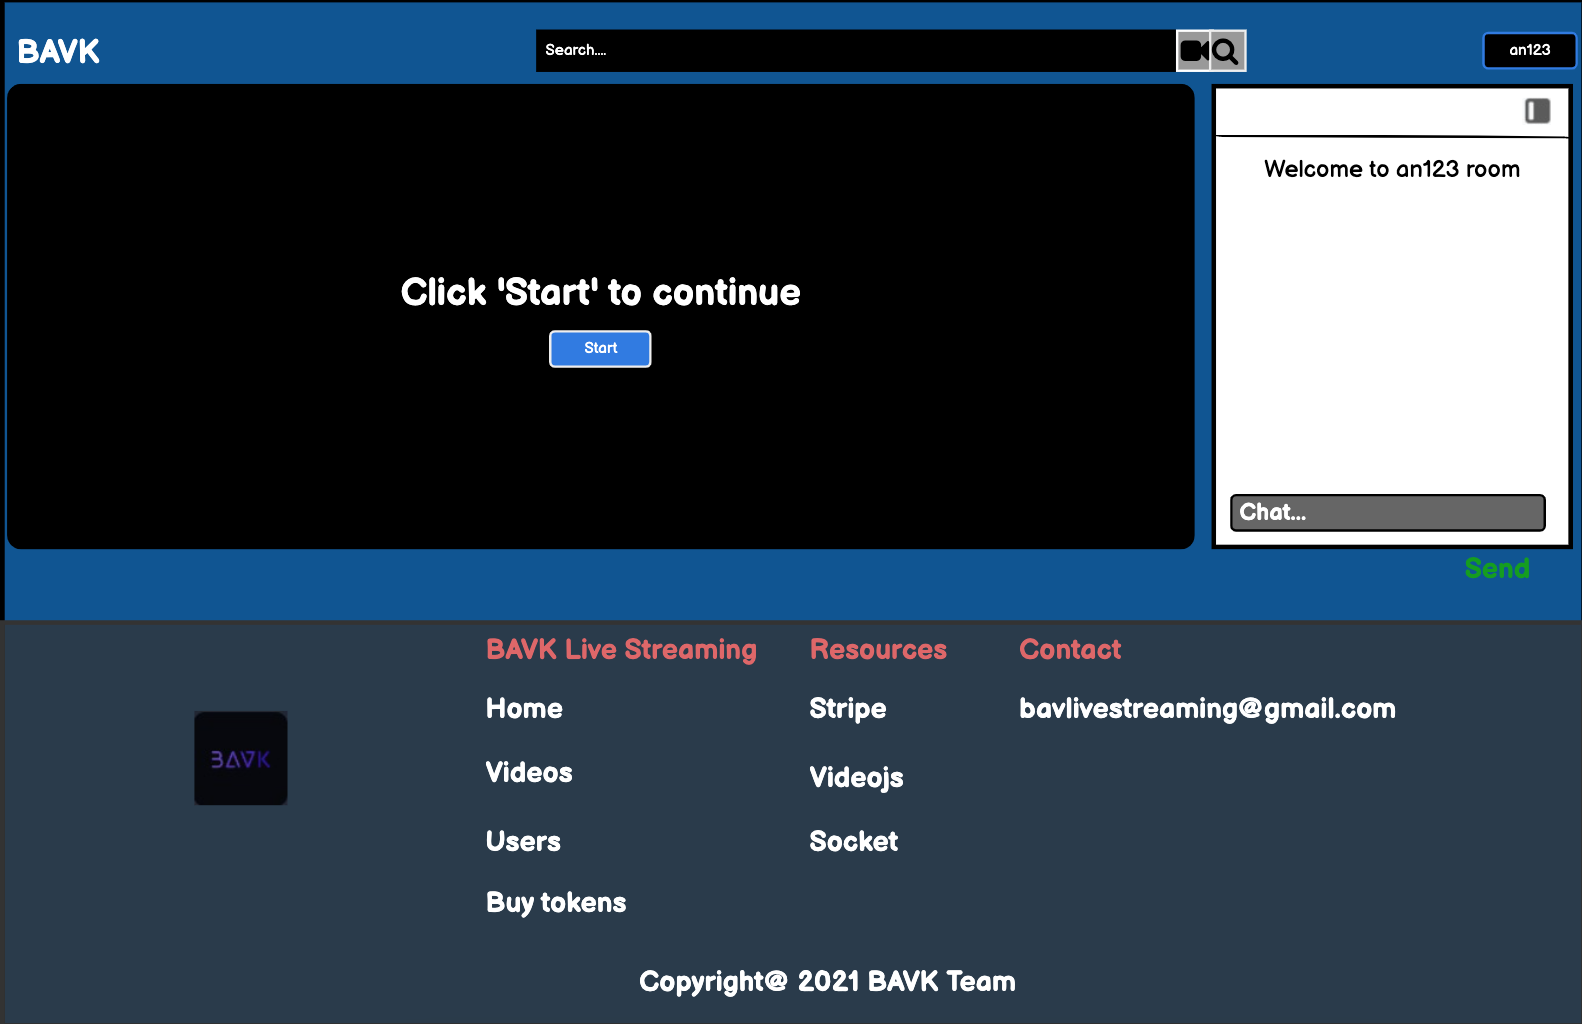
\includegraphics[width=17cm]{{./imgs/streamer_page}}
		\caption{Trang cho streamer}
	\end{figure}
	\end{center}
	
	
\begin{center}
\begin{longtabu} to \textwidth {| m{1cm} | m{4cm} | m{3cm} | m{7cm} |}
\caption{Mô tả trang streamer} \\
    \hline \textbf{STT}  & \textbf{Điều khiển} & \textbf{Sự kiện} & \textbf{Mô tả} \\ \hline
    \endfirsthead
    \hline \textbf{STT}  & \textbf{Điều khiển} & \textbf{Sự kiện} & \textbf{Mô tả} \\ \hline
    \endhead
      1 & Video manager  & Initialize & Hiển thị nội dung webcam thu được/ Hiển thị khu vực để stream trên màn hình \\
      \hline
      2 & Chat panel & Input/Click & Hiển thị các tin nhắn của tất cả người dùng trong kênh stream và cho phép người streamer tương tác với viewer \\
      \hline
      3 & Media player navigator & Click & Cho phép tin nhắn hiển thị trân màn hình stream, tắt/bật mic, cho phép truyền âm thanh, tắt/bật webcam 
      \\ \hline
       4 & Thông tin đang live stream & Initialize & Cho phép xem thông tin tiêu đề, số lượt xem, số lượng yêu thích, tổng thời gian đã live stream, các users đang bị lock chat
      \\ \hline
      5 & Ghi hình & Click & Cho phép streamer ghi hình lại video và sau đó có thể thiết lập các thông tin cần thiết để lưu video
      \\ \hline
\end{longtabu}
\end{center}
	

	\begin{center}
	\begin{figure}[H]
		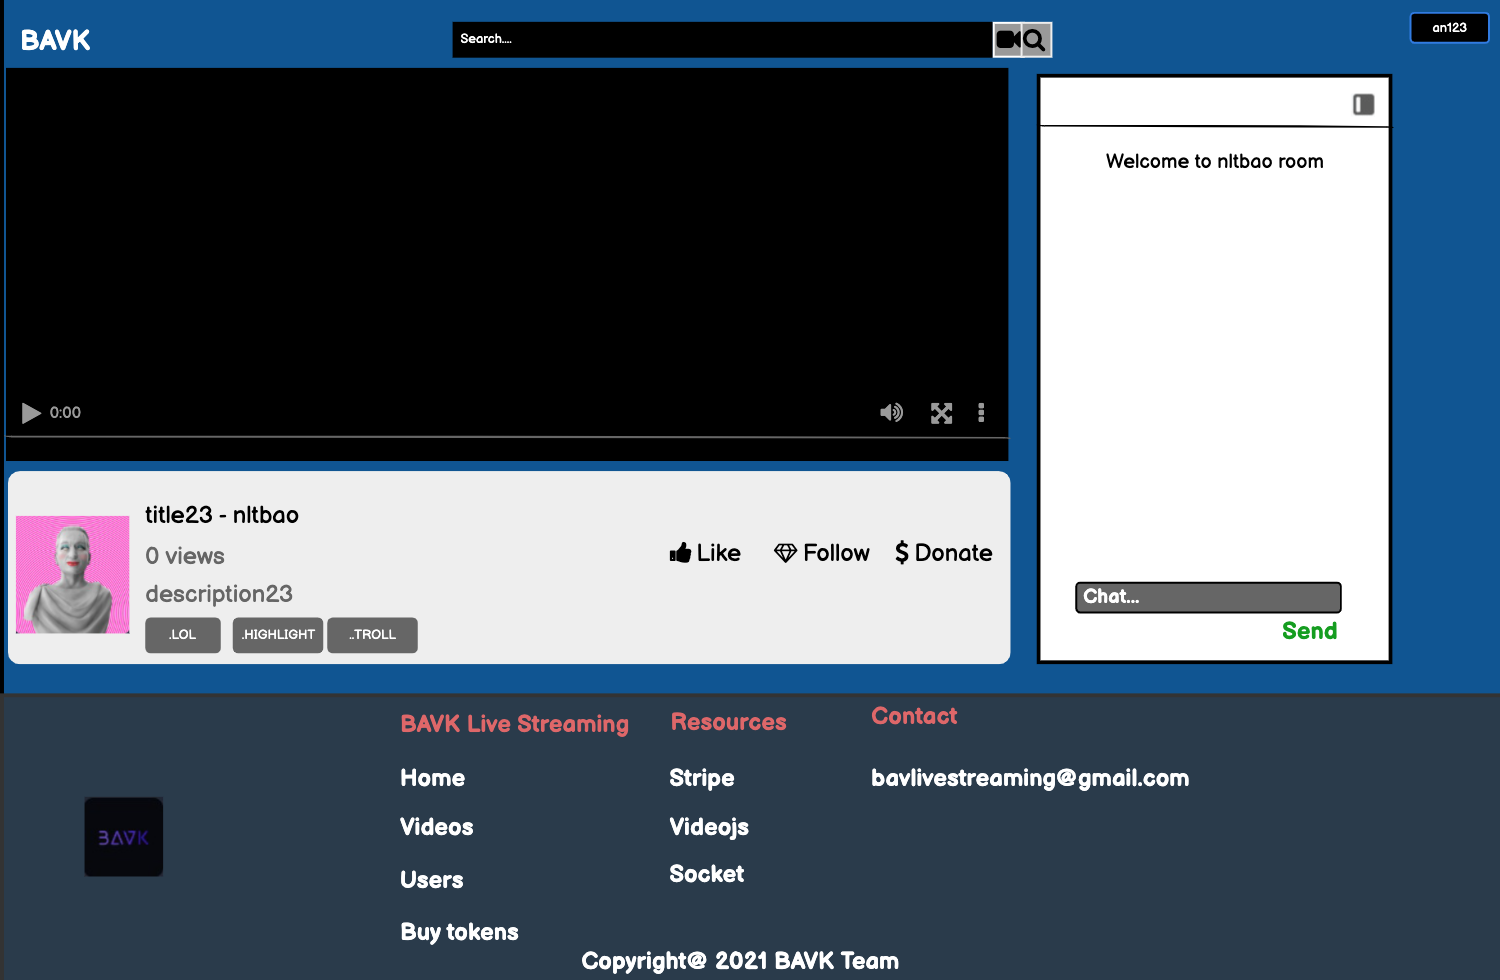
\includegraphics[width=17cm]{{./imgs/viewer_page}}
		\caption{Trang cho viewer}
	\end{figure}
	\end{center}

\begin{center}
\begin{longtabu} to \textwidth {| m{1cm} | m{4cm} | m{3cm} | m{7cm} |}
\caption{Mô tả trang viewer} \\
    \hline \textbf{STT}  & \textbf{Điều khiển} & \textbf{Sự kiện} & \textbf{Mô tả} \\ \hline
    \endfirsthead
    \hline \textbf{STT}  & \textbf{Điều khiển} & \textbf{Sự kiện} & \textbf{Mô tả} \\ \hline
    \endhead
      1 & Video player  & Initialize & Hiển thị hình ảnh đang được streamer chia sẻ \\
      \hline
      2 & Chat panel & Input/Click & Hiển thị các tin nhắn của tất cả người dùng trong kênh stream và cho phép người viewer tương tác với tất cả \\
      \hline
      3 & Streamer info & Click & Cho phép viewer theo dõi thông tin của streamer được chọn \\
      \hline
      4 & Subscribe button & Click & Đăng ký kênh, viewer sẽ nhận được các thông báo về các sự kiện liên quan của streamer khi có video \\
      \hline
      5 & Like video button & Click & Thích video đang xem  \\
      \hline
\end{longtabu}
\end{center}


	\begin{center}
	\begin{figure}[H]
		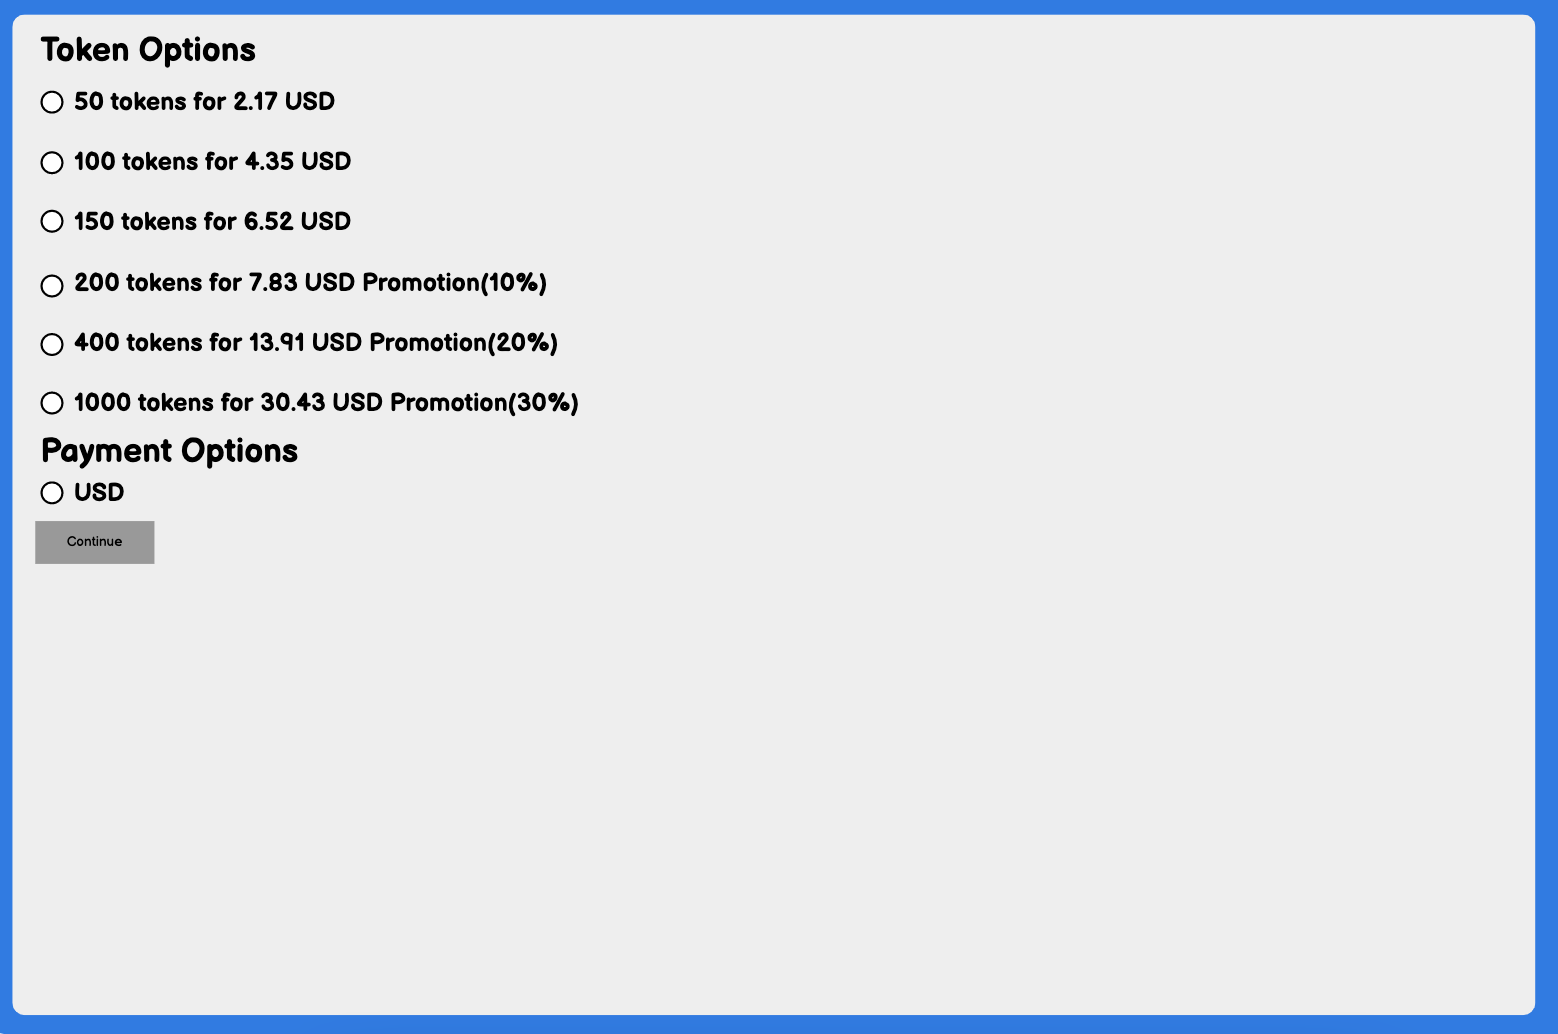
\includegraphics[width=17cm,height=15cm]{{./imgs/purchase_page}}
		\caption{Trang mua token}
	\end{figure}
	\end{center}
	
\begin{center}
\begin{longtabu} to \textwidth {| m{1cm} | m{4cm} | m{3cm} | m{7cm} |}
\caption{Mô tả trang mua token} \\
   \hline \textbf{STT}  & \textbf{Điều khiển} & \textbf{Sự kiện} & \textbf{Mô tả} \\ \hline
    \endfirsthead
    \hline \textbf{STT}  & \textbf{Điều khiển} & \textbf{Sự kiện} & \textbf{Mô tả} \\ \hline
    \endhead
      1 & Số lượng token muốn mua & Click & Người dùng có thể chọn số lượng token và đơn vị tiền tệ (USD) để thanh toán \\
      \hline
      2 & Tiến hành thanh toán & Input/Click & Người dùng thanh toán qua VISA \\
      \hline
\end{longtabu}
\end{center}


	\begin{center}
	\begin{figure}[H]
		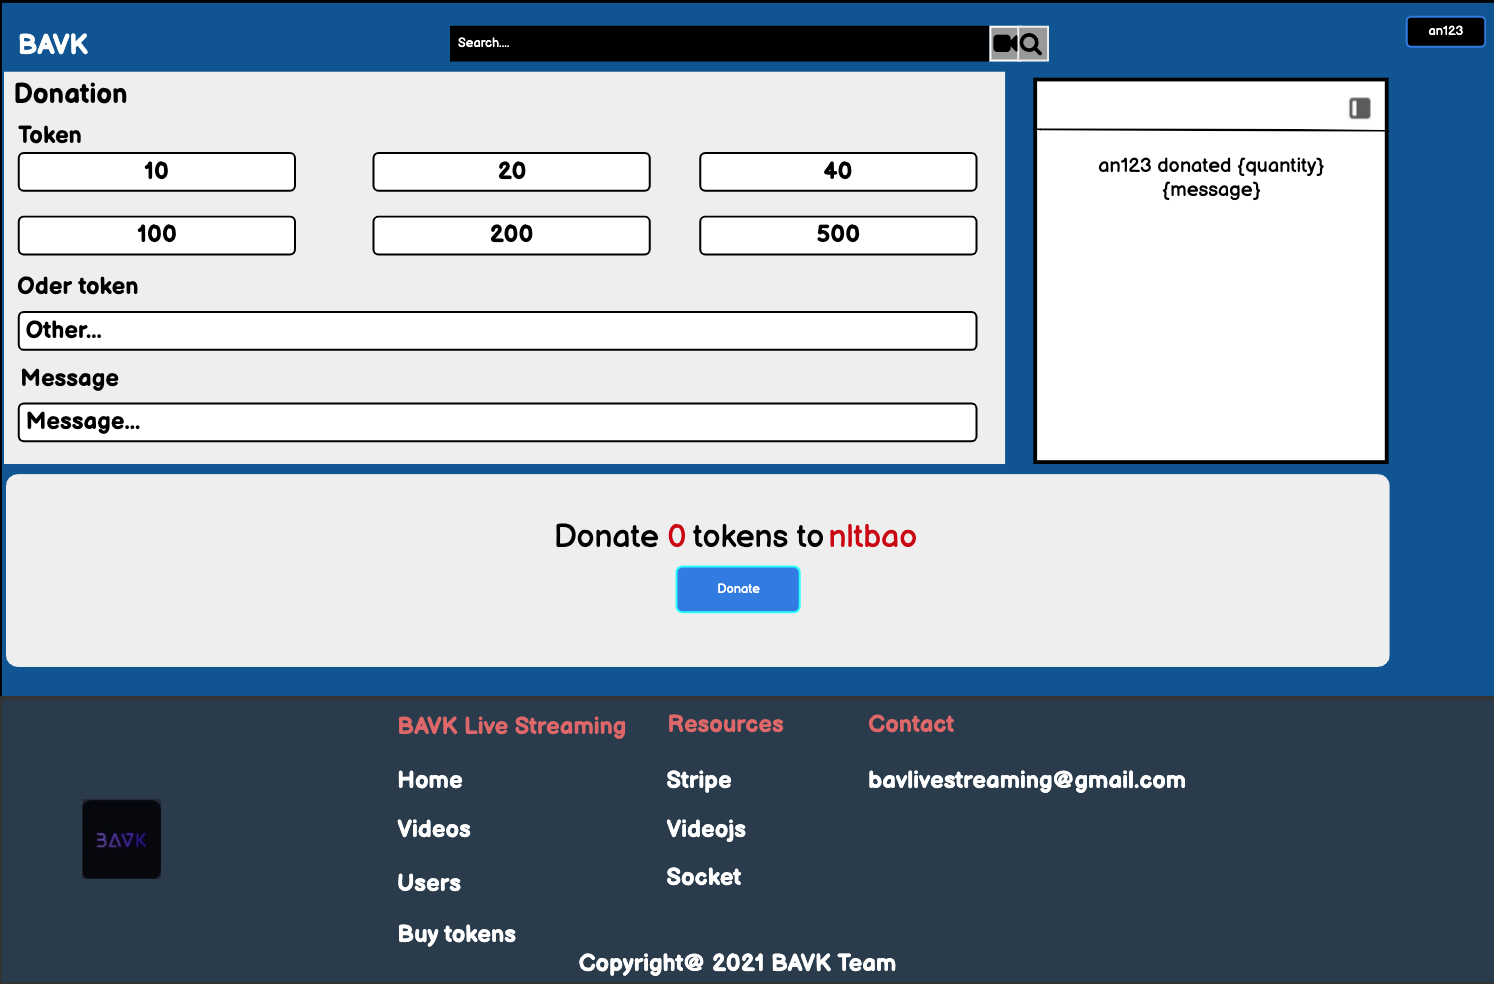
\includegraphics[width=17cm]{{./imgs/donate_page}}
		\caption{Trang donate}
	\end{figure}
	\end{center}
	
\begin{center}
\begin{longtabu} to \textwidth {| m{1cm} | m{4cm} | m{3cm} | m{7cm} |}
\caption{Mô tả trang donate} \\
    \hline \textbf{STT}  & \textbf{Điều khiển} & \textbf{Sự kiện} & \textbf{Mô tả} \\ \hline
    \endfirsthead
    \hline \textbf{STT}  & \textbf{Điều khiển} & \textbf{Sự kiện} & \textbf{Mô tả} \\ \hline
    \endhead
      1 & Số lượng token donate & Click & Cho phép nhân viên chọn số lượng token để đonate cho streamer(Số lượng donate phải phù hợp với số lượng token đang có) \\
      \hline
      2 & Tin nhắn gửi tới streamer & Input  & Cho phép người dùng gửi token đính kèm tin nhắn tới cho streamer \\
      \hline
      3 & Donate & Click & Sau khi donate, thông tin donate sẽ gửi trực tiếp broadcast tới phòng của streamer. Streamer và các viewer đều có thể thấy được tin nhắn \\
      \hline
\end{longtabu}
\end{center}	
	
	
	\begin{center}
	\begin{figure}[H]
		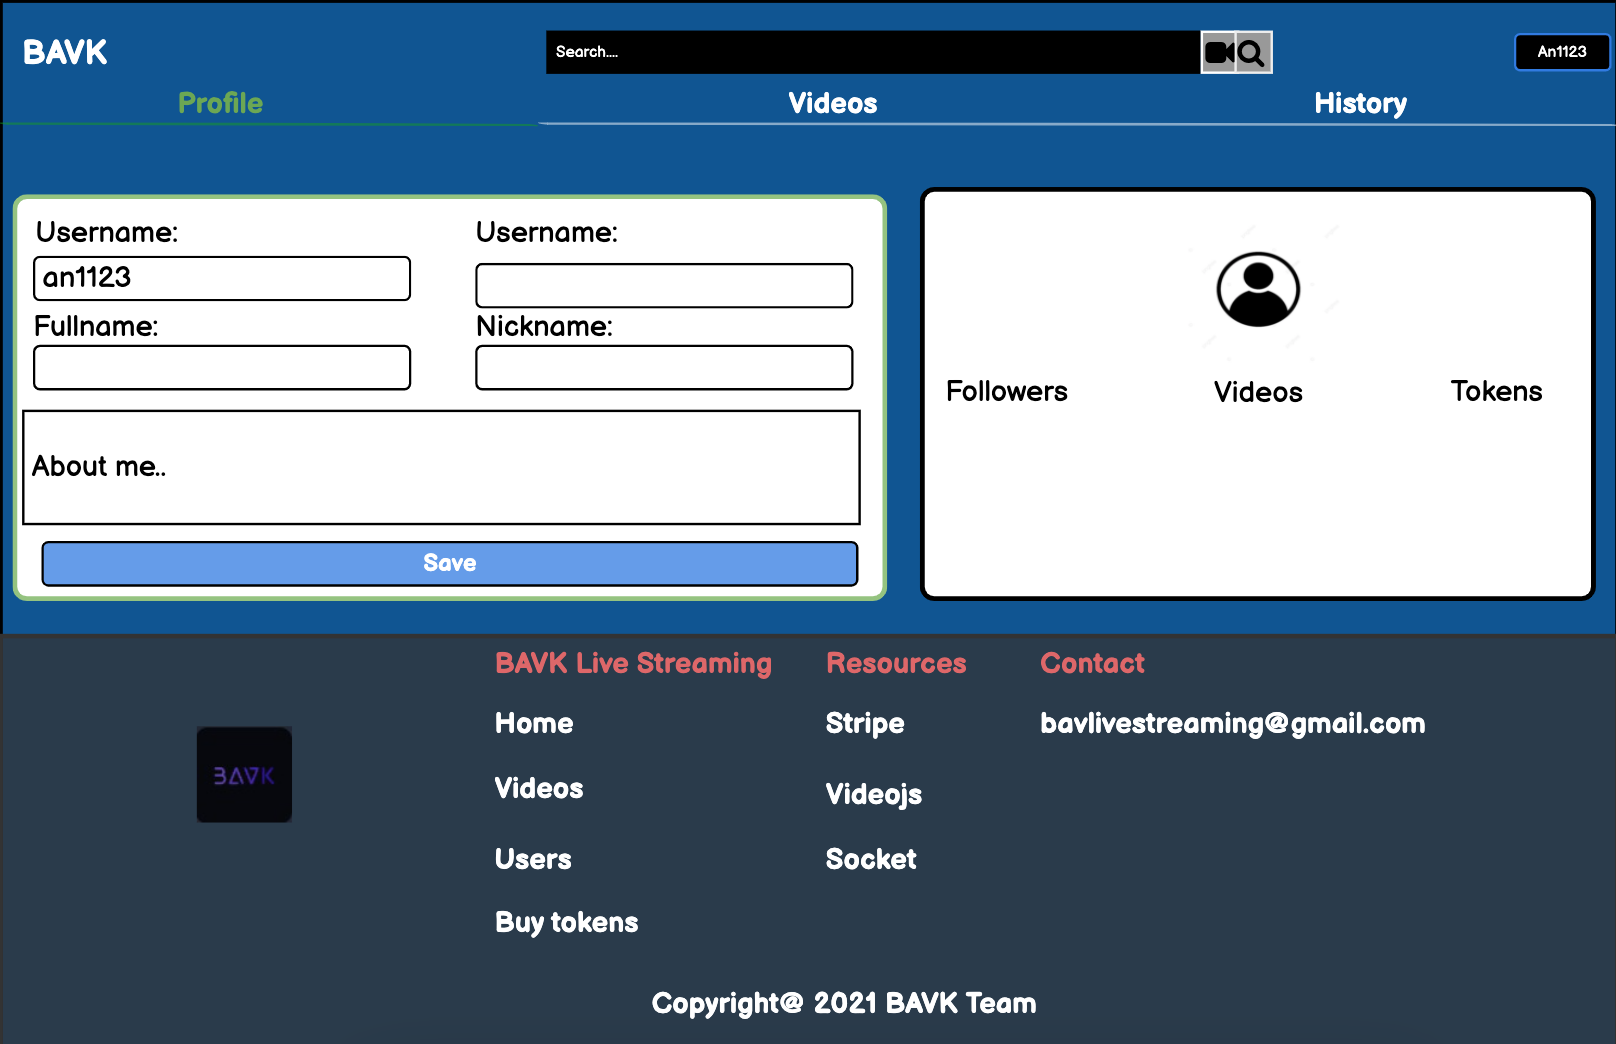
\includegraphics[width=17cm]{{./imgs/profile_page}}
		\caption{Trang hồ sơ}
	\end{figure}
	\end{center}
	
\begin{center}
\begin{longtabu} to \textwidth {| m{1cm} | m{4cm} | m{3cm} | m{7cm} |}
\caption{Mô tả trang thông tin cá nhân} \\
    \hline \textbf{STT}  & \textbf{Điều khiển} & \textbf{Sự kiện} & \textbf{Mô tả} \\ \hline
    \endfirsthead
    \hline \textbf{STT}  & \textbf{Điều khiển} & \textbf{Sự kiện} & \textbf{Mô tả} \\ \hline
    \endhead
      1 & Xem và thay đổi thông tin hồ sơ  & Initialize & Cho phép người dùng thay đổi thông tin \\
      \hline
      2 & Lưu hồ sơ& Click & Tiến hành thay đổi thông tin \\
      \hline
\end{longtabu}
\end{center}	


	\begin{center}
	\begin{figure}[H]
		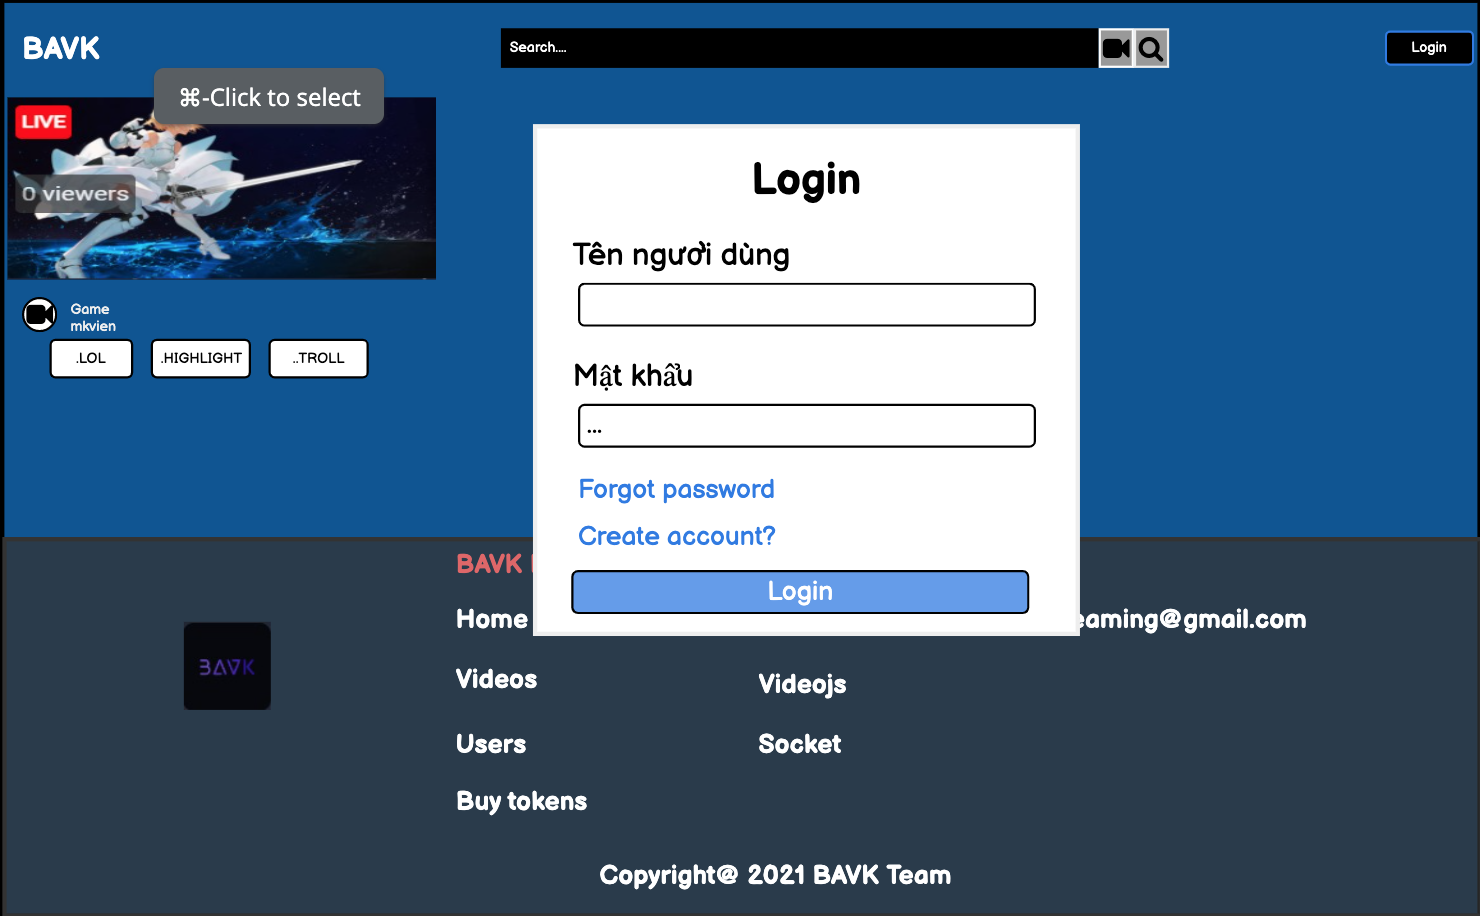
\includegraphics[width=17cm]{{./imgs/login_page}}
		\caption{Trang đăng nhập}
	\end{figure}
	\end{center}
	\begin{center}
	\begin{figure}[H]
		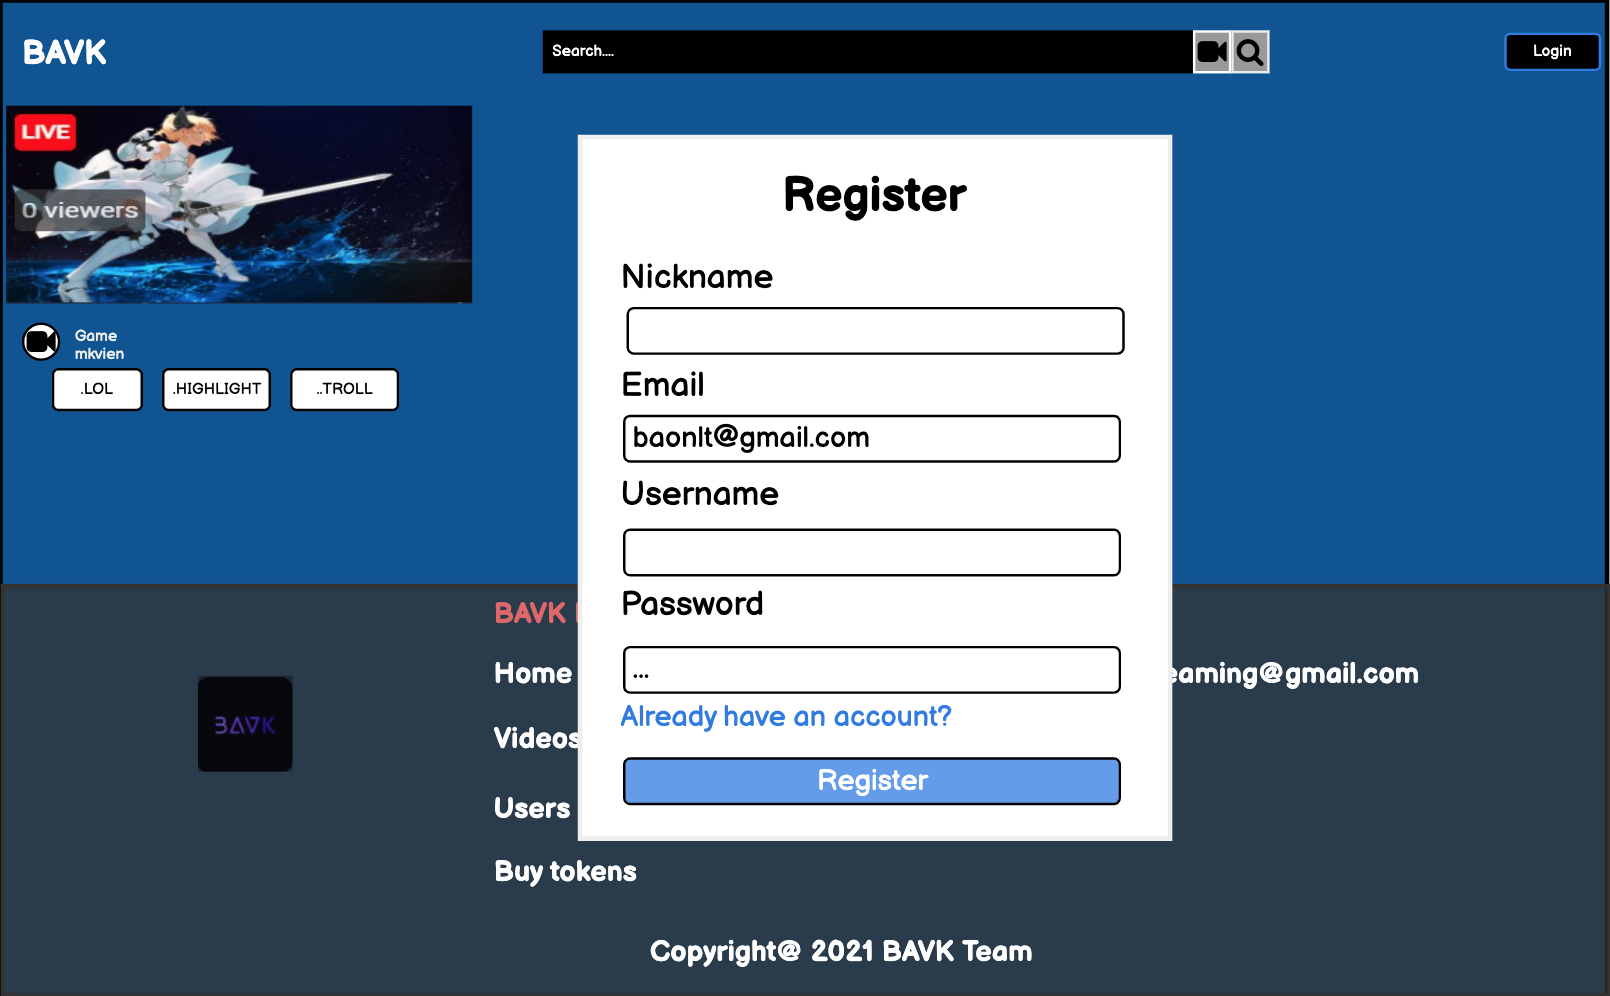
\includegraphics[width=17cm]{{./imgs/register_page}}
		\caption{Trang đăng ký}
	\end{figure}
	\end{center}
	
\begin{center}
\begin{longtabu} to \textwidth {| m{1cm} | m{4cm} | m{3cm} | m{7cm} |}
\caption{Mô tả dialog Đăng nhập/Đăng ký/Đổi mật khẩu} \\
    \hline \textbf{STT}  & \textbf{Điều khiển} & \textbf{Sự kiện} & \textbf{Mô tả} \\ \hline
    \endfirsthead
    \hline \textbf{STT}  & \textbf{Điều khiển} & \textbf{Sự kiện} & \textbf{Mô tả} \\ \hline
    \endhead
      1 & Username & Input & Tên đăng nhập \\
      \hline
      2 & Password & Input & Mật khẩu đăng nhập \\
      \hline
      3 & Email & Input & Địa chỉ email \\
      \hline
      4 & Username & Input & Tên đăng nhập \\
      \hline
\end{longtabu}
\end{center}
	
	
	\begin{center}
	\begin{figure}[H]
		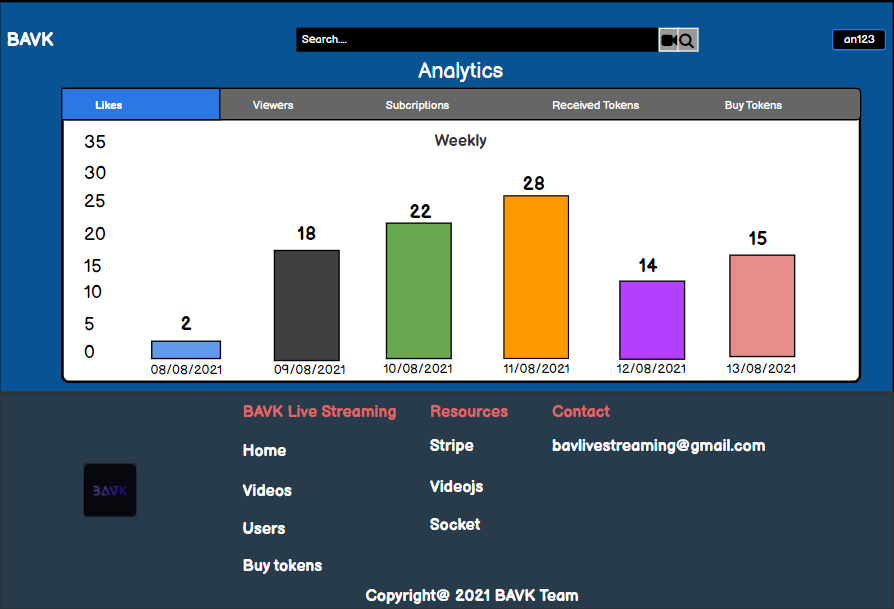
\includegraphics[width=17cm]{{./imgs/analytics}}
		\caption{Trang thống kê}
	\end{figure}
	\end{center}
	
\begin{center}
\begin{longtabu} to \textwidth {| m{1cm} | m{4cm} | m{3cm} | m{7cm} |}
\caption{Mô tả trang danh sách người dùng} \\
    \hline \textbf{STT}  & \textbf{Điều khiển} & \textbf{Sự kiện} & \textbf{Mô tả} \\ \hline
    \endfirsthead
    \hline \textbf{STT}  & \textbf{Điều khiển} & \textbf{Sự kiện} & \textbf{Mô tả} \\ \hline
    \endhead
      1 & Thống kê giao dịch ngân hàng & Initialize & So sánh số lượng tiền nạp vào và tiền rút ra \\
      \hline
      2 & Thống kê donate & Initialize & So sánh số lượng token được donate và donate\\
      \hline
       3 & Thống kê thông tin chung & Initialize/Click & Xem dữ liệu biến động qua các mốc thời gian theo mục được chọn\\
      \hline
\end{longtabu}
\end{center}


	\begin{center}
	\begin{figure}[H]
		\includegraphics[width=17cm]{{./imgs/history_donate}}
		\caption{Trang lịch sử donate}
	\end{figure}
	\end{center}
	
\begin{center}
\begin{longtabu} to \textwidth {| m{1cm} | m{4cm} | m{3cm} | m{7cm} |}
\caption{Mô tả trang lịch sử donate} \\
    \hline \textbf{STT}  & \textbf{Điều khiển} & \textbf{Sự kiện} & \textbf{Mô tả} \\ \hline
    \endfirsthead
    \hline \textbf{STT}  & \textbf{Điều khiển} & \textbf{Sự kiện} & \textbf{Mô tả} \\ \hline
    \endhead
      1 & Xem lịch sử  & Initialize & Cho phép người dùng xem thông tin lịch sử donate\\
      \hline
\end{longtabu}
\end{center}

	\begin{center}
	\begin{figure}[H]
		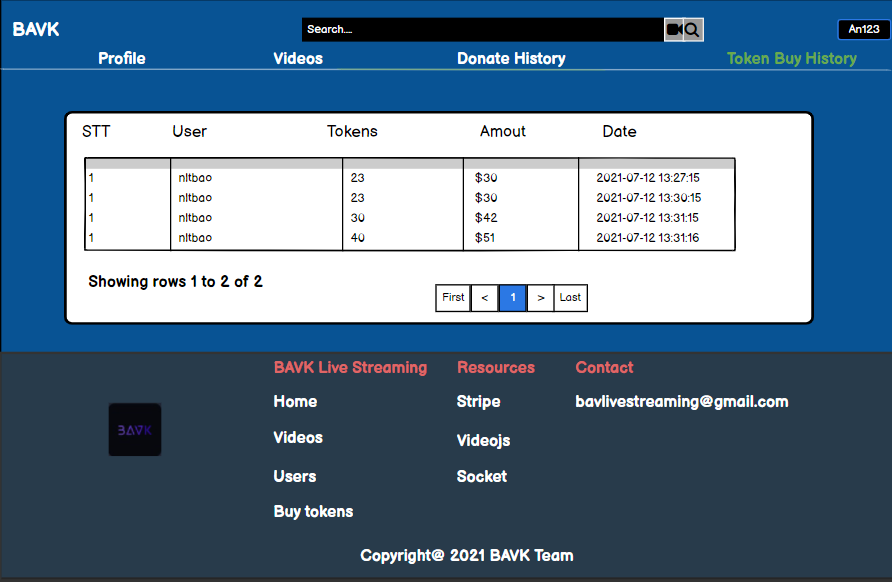
\includegraphics[width=17cm]{{./imgs/history_token}}
		\caption{Trang lịch sử token}
	\end{figure}
	\end{center}

\begin{center}
\begin{longtabu} to \textwidth {| m{1cm} | m{4cm} | m{3cm} | m{7cm} |}
\caption{Mô tả trang lịch sử token} \\
    \hline \textbf{STT}  & \textbf{Điều khiển} & \textbf{Sự kiện} & \textbf{Mô tả} \\ \hline
    \endfirsthead
    \hline \textbf{STT}  & \textbf{Điều khiển} & \textbf{Sự kiện} & \textbf{Mô tả} \\ \hline
    \endhead
      1 & Xem lịch sử  & Initialize & Cho phép người dùng xem thông tin lịch sử mua token\\
      \hline
\end{longtabu}
\end{center}

	\begin{center}
	\begin{figure}[H]
		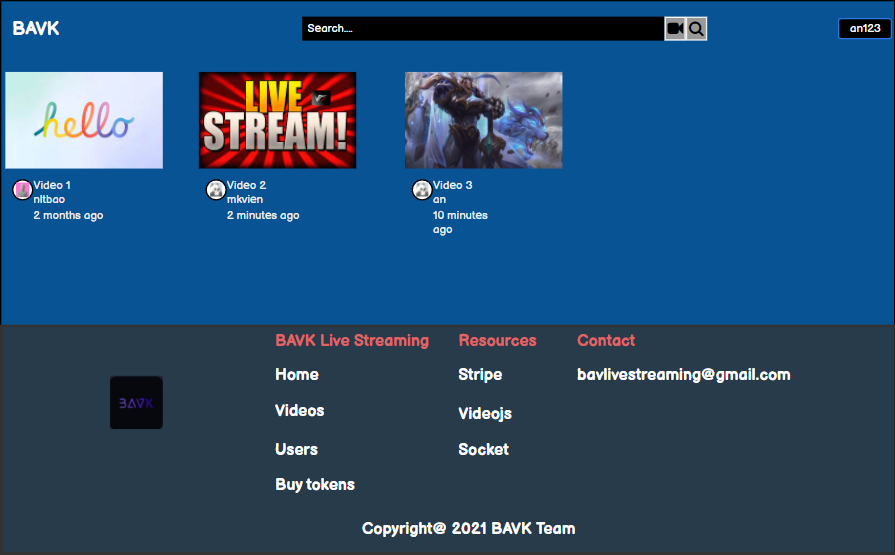
\includegraphics[width=17cm]{{./imgs/page_video.png}}
		\caption{Trang danh sách video}
	\end{figure}
	\end{center}

\begin{center}
\begin{longtabu} to \textwidth {| m{1cm} | m{4cm} | m{3cm} | m{7cm} |}
\caption{Mô tả trang danh sách videos} \\
    \hline \textbf{STT}  & \textbf{Điều khiển} & \textbf{Sự kiện} & \textbf{Mô tả} \\ \hline
    \endfirsthead
    \hline \textbf{STT}  & \textbf{Điều khiển} & \textbf{Sự kiện} & \textbf{Mô tả} \\ \hline
    \endhead
      1 & Danh sách video  & Initialize & Hiển thị các video được tạo ra từ ghi hình của user\\
      \hline
      2 & Thay đổi thông tin video & Click/Input & Cho phép user thay đổi tiêu đề của video \\
      \hline
\end{longtabu}
\end{center}

	\begin{center}
	\begin{figure}[H]
		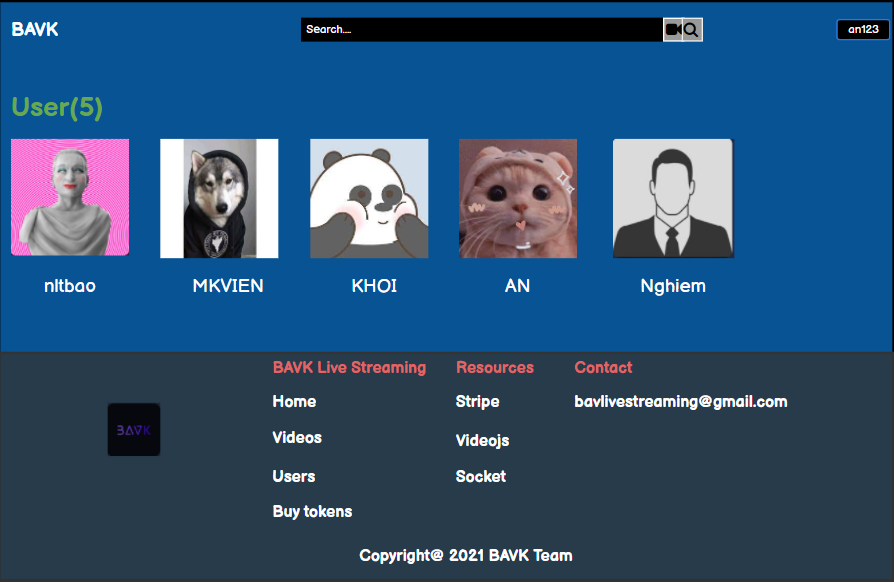
\includegraphics[width=17cm]{{./imgs/page_user}}
		\caption{Trang danh sách người dùng}
	\end{figure}
	\end{center}

\begin{center}
\begin{longtabu} to \textwidth {| m{1cm} | m{4cm} | m{3cm} | m{7cm} |}
\caption{Mô tả trang danh sách người dùng} \\
    \hline \textbf{STT}  & \textbf{Điều khiển} & \textbf{Sự kiện} & \textbf{Mô tả} \\ \hline
    \endfirsthead
    \hline \textbf{STT}  & \textbf{Điều khiển} & \textbf{Sự kiện} & \textbf{Mô tả} \\ \hline
    \endhead
      1 & Danh sách người dùng  & Initialize & Hiển thị toàn bộ danh sách người dùng \\
      \hline
      2 & Xem thông tin hồ sơ người dùng & Click & Điều hướng tới trang hồ sơ của người dùng \\
      \hline
\end{longtabu}
\end{center}


\section{Thiết Kế Dữ Liệu}
\subsection{Sơ đồ thực thể ERD}
\subsubsection{Tổng quan ERD}
	\begin{center}
		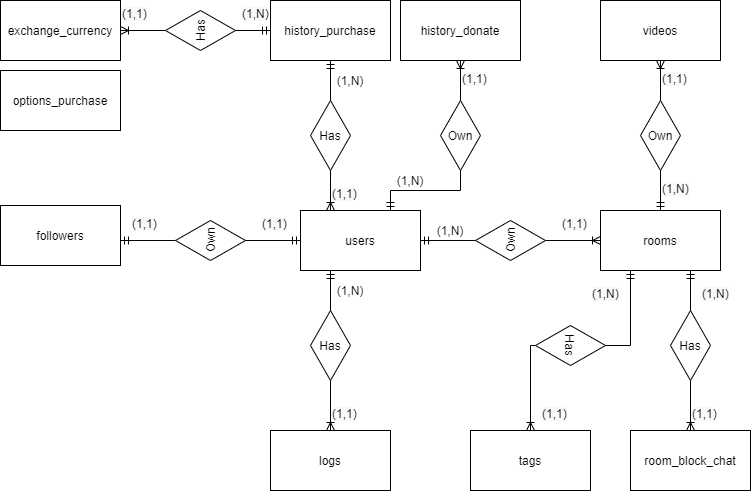
\includegraphics[width=17cm]{{./imgs/erd_overview}}
	\end{center}
	
\subsubsection{Chi tiết ERD}
	\begin{center}
		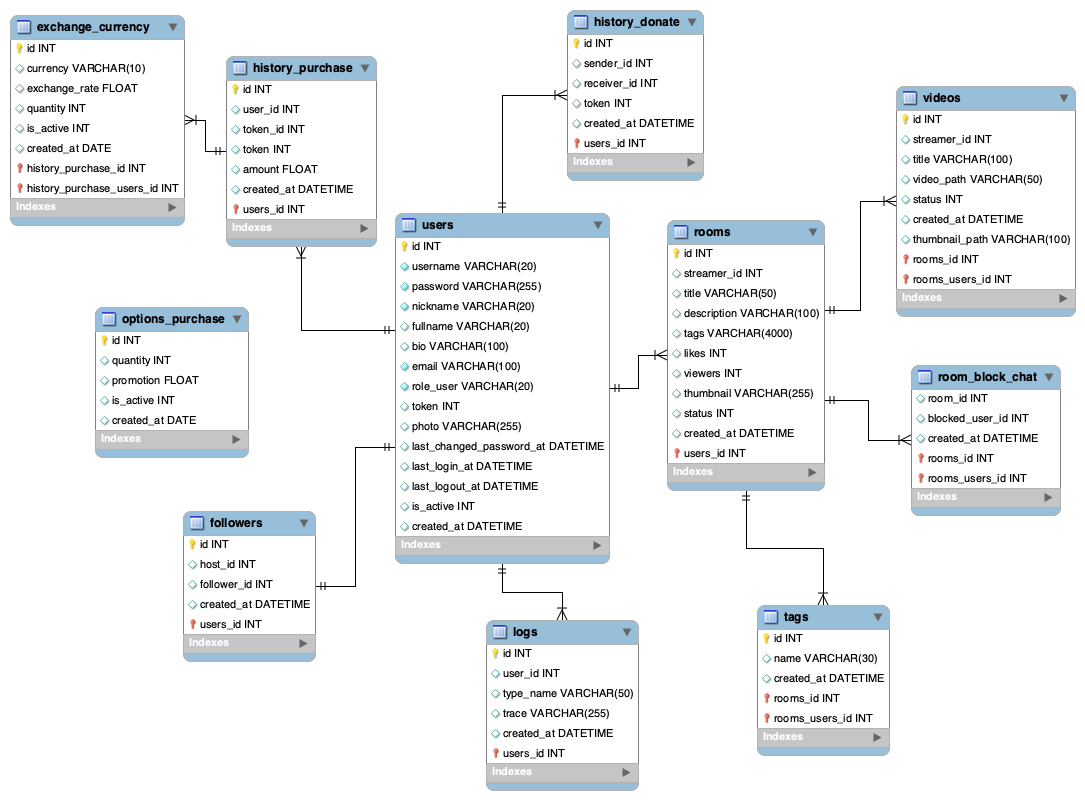
\includegraphics[width=17cm]{{./imgs/erd}}
	\end{center}
	
\subsubsection{Chi tiết các thực thể}


%%%%%%%% USERS %%%%%%%%
\begin{center}
\begin{longtabu} to \textwidth {| m{3cm} | m{3cm} | m{5cm} | m{4cm} |}
\caption{Thực thể Users} \\
   \hline \textbf{Thuộc tính}  & \textbf{Kiểu} & \textbf{Mô tả} & \textbf{Ràng buộc} \\ \hline
   \endfirsthead
   \hline \textbf{Thuộc tính}  & \textbf{Kiểu} & \textbf{Mô tả} & \textbf{Ràng buộc} \\ \hline
   \endhead
      id & int  & Mã loại & PK,Tự tăng
      \\ \hline
      username & varchar(20) & Tên đăng nhập & NOT NULL 
      \\ \hline
      password & varchar(255) & Mật khẩu đăng nhập & NOT NULL
      \\ \hline
      nickname & nvarchar(20) & Biệt danh & NOT NULL
      \\ \hline
      fullname & nvarchar(20) & Họ và tên & NULL
      \\ \hline
      role\_user & varchar(20) & Vai trò người dùng& NOT NULL
      \\ \hline
      token & int & Tổng số \quotes{xèng} & NOT NULL
      \\ \hline
      email & varchar(20) & Email người dùng & NOT NULL
      \\ \hline
      gender & nvarchar(10) & Giới tính & NULL
      \\ \hline
      mobile & varchar(20) & Số điện thoại & NULL
      \\ \hline
      photo & varchar(100) & Ảnh avatar & NULL
      \\ \hline
      address & nvarchar(100) & Địa chỉ & NULL
      \\ \hline
      birthday & date & Ngày sinh & NULL
      \\ \hline
      last\_login\_at & datetime & Thời điểm lần cuối đăng nhập & NULL
      \\ \hline
      last\_logout\_at & datetime & Thời điểm lần cuối đăng xuất & NULL
      \\ \hline
      last\_changed \_password\_at & datetime & Thời điểm lần cuối đổi mật khẩu & NULL
      \\ \hline
      is\_active & int & Trạng thái tài khoản & NOT NULL
      \\ \hline
\end{longtabu}
\end{center}


%%%%%%%% ROOMS %%%%%%%%
\begin{center}
\begin{longtabu} to \textwidth {| m{3cm} | m{3cm} | m{5cm} | m{4cm} |}
\caption{Thực thể Rooms} \\
   \hline \textbf{Thuộc tính}  & \textbf{Kiểu} & \textbf{Mô tả} & \textbf{Ràng buộc} \\ \hline
   \endfirsthead
   \hline \textbf{Thuộc tính}  & \textbf{Kiểu} & \textbf{Mô tả} & \textbf{Ràng buộc} \\ \hline
   \endhead
      id & int  & Mã loại & PK,Tự tăng
      \\ \hline
      streamer\_id & int & Id streamer & NOT NULL 
      \\ \hline
      title & nvarchar(50) & Tiêu đề phòng & NOT NULL
      \\ \hline
      description & nvarchar(100) & Mô tả phòng & NULL
      \\ \hline
      tags & nvarchar(max) & Chủ đề phòng & NULL
      \\ \hline
      likes & int & Số lượt yêu thích & NOT NULL
      \\ \hline
      viewers & int & Số lượt ghé thăm & NOT NULL
      \\ \hline
      thumbnail & varchar(100) & Snapshot của phòng & NOT NULL
      \\ \hline
      status & int & Trạng thái phòng & NOT NULL
      \\ \hline
      created\_at & datetime & Ngày tạo & NOT NULL
      \\ \hline
\end{longtabu}
\end{center}

%%%%%%%% VIDEOS %%%%%%%%
\begin{center}
\begin{longtabu} to \textwidth {| m{3cm} | m{3cm} | m{5cm} | m{4cm} |}
\caption{Thực thể Videos} \\
   \hline \textbf{Thuộc tính}  & \textbf{Kiểu} & \textbf{Mô tả} & \textbf{Ràng buộc} \\ \hline
   \endfirsthead
   \hline \textbf{Thuộc tính}  & \textbf{Kiểu} & \textbf{Mô tả} & \textbf{Ràng buộc} \\ \hline
   \endhead
      id & int  & Mã loại & PK,Tự tăng
      \\ \hline
      streamer\_id & int & Id streamer & NOT NULL 
      \\ \hline
      title & nvarchar(50) & Tiêu đề phòng & NOT NULL
      \\ \hline
      video\_path & varchar(100) & Đường dẫn tới video & NOT NULL
      \\ \hline
      status & int & Trạng thái video & NOT NULL
      \\ \hline
      created\_at & datetime & Ngày tạo & NOT NULL
      \\ \hline
\end{longtabu}
\end{center}

%%%%%%%% ROOM_BLOCK_CHAT %%%%%%%%
\begin{center}
\begin{longtabu} to \textwidth {| m{3cm} | m{3cm} | m{5cm} | m{4cm} |}
\caption{Thực thể Room Block Chat} \\
   \hline \textbf{Thuộc tính}  & \textbf{Kiểu} & \textbf{Mô tả} & \textbf{Ràng buộc} \\ \hline
   \endfirsthead
   \hline \textbf{Thuộc tính}  & \textbf{Kiểu} & \textbf{Mô tả} & \textbf{Ràng buộc} \\ \hline
   \endhead
      room\_id & int & Mã loại  & PK,Tự tăng
      \\ \hline
      blocked\_userId & int & Id user & NOT NULL
      \\ \hline
      created\_at & datetime & Ngày tạo & NOT NULL
      \\ \hline
\end{longtabu}
\end{center}

%%%%%%%% TAGS %%%%%%%%
\begin{center}
\begin{longtabu} to \textwidth {| m{3cm} | m{3cm} | m{5cm} | m{4cm} |}
\caption{Thực thể Tags} \\
   \hline \textbf{Thuộc tính}  & \textbf{Kiểu} & \textbf{Mô tả} & \textbf{Ràng buộc} \\ \hline
   \endfirsthead
   \hline \textbf{Thuộc tính}  & \textbf{Kiểu} & \textbf{Mô tả} & \textbf{Ràng buộc} \\ \hline
   \endhead
      id & int  & Mã loại & PK,Tự tăng
      \\ \hline
      name & nvarchar(20) & Tên chủ đề & NOT NULL 
      \\ \hline
      created\_at & datetime & Ngày tạo & NOT NULL
      \\ \hline
\end{longtabu}
\end{center}

%%%%%%%% HISTORY DONATE %%%%%%%%
\begin{center}
\begin{longtabu} to \textwidth {| m{3cm} | m{3cm} | m{5cm} | m{4cm} |}
\caption{Thực thể History Donate} \\
   \hline \textbf{Thuộc tính}  & \textbf{Kiểu} & \textbf{Mô tả} & \textbf{Ràng buộc} \\ \hline
   \endfirsthead
   \hline \textbf{Thuộc tính}  & \textbf{Kiểu} & \textbf{Mô tả} & \textbf{Ràng buộc} \\ \hline
   \endhead
      id & int  & Mã loại & PK,Tự tăng
      \\ \hline
      sender\_id & int & Id người gửi & NOT NULL 
      \\ \hline
      receiver\_id & int & Id người nhận  & NOT NULL 
      \\ \hline
      token & int & Số lượng \quotes{Xèng} & NOT NULL
      \\ \hline
      created\_at & datetime & Ngày tạo & NOT NULL
      \\ \hline
\end{longtabu}
\end{center}

%%%%%%%% HISTORY PURCHASE %%%%%%%%
\begin{center}
\begin{longtabu} to \textwidth {| m{3cm} | m{3cm} | m{5cm} | m{4cm} |}
\caption{Thực thể History Purchase} \\
   \hline \textbf{Thuộc tính}  & \textbf{Kiểu} & \textbf{Mô tả} & \textbf{Ràng buộc} \\ \hline
   \endfirsthead
   \hline \textbf{Thuộc tính}  & \textbf{Kiểu} & \textbf{Mô tả} & \textbf{Ràng buộc} \\ \hline
   \endhead
      id & int  & Mã loại & PK,Tự tăng
      \\ \hline
      user\_id & int & Id người dùng & NOT NULL 
      \\ \hline
      token\_id & int & Id tỉ giá tiền tệ  & NOT NULL 
      \\ \hline
      amount & float & Số tiền & NOT NULL
       \\ \hline
      token & int & Số lượng \quotes{Xèng} & NOT NULL
      \\ \hline
      created\_at & datetime & Ngày tạo & NOT NULL
      \\ \hline
\end{longtabu}
\end{center}

%%%%%%%% EXCHANGE CURRENCY %%%%%%%%
\begin{center}
\begin{longtabu} to \textwidth {| m{3cm} | m{3cm} | m{5cm} | m{4cm} |}
\caption{Thực thể Exchange Currency} \\
   \hline \textbf{Thuộc tính}  & \textbf{Kiểu} & \textbf{Mô tả} & \textbf{Ràng buộc} \\ \hline
   \endfirsthead
   \hline \textbf{Thuộc tính}  & \textbf{Kiểu} & \textbf{Mô tả} & \textbf{Ràng buộc} \\ \hline
   \endhead
      id & int  & Mã loại & PK,Tự tăng
      \\ \hline
      currency & varchar(10) & Đơn vị tiền tệ (USD,VND,...) & NOT NULL 
      \\ \hline
      exchange\_rate & float & Tỉ giá tiền tệ  & NOT NULL 
      \\ \hline
      quantity & int & Số \quotes{Xèng} dự vào tỉ giá & NOT NULL
       \\ \hline
      is\_active & int & Trạng thái & NOT NULL
      \\ \hline
      created\_at & datetime & Ngày tạo & NOT NULL
      \\ \hline
\end{longtabu}
\end{center}

%%%%%%%% OPTION PURCHASE %%%%%%%%
\begin{center}
\begin{longtabu} to \textwidth {| m{3cm} | m{3cm} | m{5cm} | m{4cm} |}
\caption{Thực thể Option Purchase} \\
   \hline \textbf{Thuộc tính}  & \textbf{Kiểu} & \textbf{Mô tả} & \textbf{Ràng buộc} \\ \hline
   \endfirsthead
   \hline \textbf{Thuộc tính}  & \textbf{Kiểu} & \textbf{Mô tả} & \textbf{Ràng buộc} \\ \hline
   \endhead
      id & int  & Mã loại & PK,Tự tăng
      \\ \hline
      quantity & int & Số \quotes{Xèng} & NOT NULL
      \\ \hline
      promotion & float & Phần trăm khuyến mãi & NOT NULL 
       \\ \hline
      is\_active & int & Trạng thái & NOT NULL
      \\ \hline
      created\_at & datetime & Ngày tạo & NOT NULL
      \\ \hline
\end{longtabu}
\end{center}

%%%%%%%% FOLLOWERS  %%%%%%%%
\begin{center}
\begin{longtabu} to \textwidth {| m{3cm} | m{3cm} | m{5cm} | m{4cm} |}
\caption{Thực thể Followers} \\
   \hline \textbf{Thuộc tính}  & \textbf{Kiểu} & \textbf{Mô tả} & \textbf{Ràng buộc} \\ \hline
   \endfirsthead
   \hline \textbf{Thuộc tính}  & \textbf{Kiểu} & \textbf{Mô tả} & \textbf{Ràng buộc} \\ \hline
   \endhead
      id & int  & Mã loại & PK,Tự tăng
      \\ \hline
      host\_id & int & Id người dùng được theo dõi & NOT NULL
      \\ \hline
      follower\_id & int & Id người dùng theo dõi & NOT NULL 
       \\ \hline
      created\_at & datetime & Ngày tạo & NOT NULL
      \\ \hline
\end{longtabu}
\end{center}

%%%%%%%% LOGS  %%%%%%%%
\begin{center}
\begin{longtabu} to \textwidth {| m{3cm} | m{3cm} | m{5cm} | m{4cm} |}
\caption{Thực thể Logs} \\
   \hline \textbf{Thuộc tính}  & \textbf{Kiểu} & \textbf{Mô tả} & \textbf{Ràng buộc} \\ \hline
   \endfirsthead
   \hline \textbf{Thuộc tính}  & \textbf{Kiểu} & \textbf{Mô tả} & \textbf{Ràng buộc} \\ \hline
   \endhead
      id & int  & Mã loại & PK,Tự tăng
      \\ \hline
      user\_id & int & Id người dùng & NOT NULL
      \\ \hline
      type\_name & varchar(15) & Loại truy vấn & NOT NULL 
      \\ \hline
      trace & nvarchar(max) & Payload truyền tới server & NOT NULL 
       \\ \hline
      created\_at & datetime & Ngày tạo & NOT NULL
      \\ \hline
\end{longtabu}
\end{center}


%%%%%%%%%%%%%%%%%%% Stored Procedure %%%%%%%%%%%%%%%%%%%%%%%%%

\section{Stored Procedure}

\begin{center}
	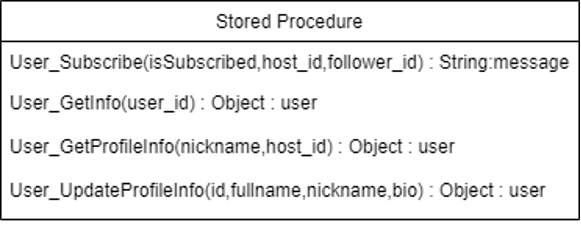
\includegraphics[width=17cm]{{./imgs/diagrams/user_procedure}}
\end{center}

\begin{center}
\begin{longtabu} to \textwidth {| m{3cm} | m{5cm} | m{4cm} | m{4cm} |}
\caption{Các trường} \\
   \hline \textbf{Tên}  & \textbf{Mô tả} & \textbf{Input} & \textbf{Output}  \\ \hline
   \endfirsthead
   \hline \textbf{Tên}  & \textbf{Mô tả} & \textbf{Input} & \textbf{Output}  \\ \hline
   \endhead
      Subscribe & Đăng ký kênh  & isSubscribed: 1 – 0, hostId: địa chỉ kênh, followerId: Id của user & Trạng thái đăng ký
      \\ \hline
      GetInfo & Lấy thông tin tài khoản  & UserId: mã Id của user & Thông tin tài khoản đăng nhập
      \\ \hline
      GetProfileInfo & Lấy thông tin user khác  & Nickname: tên nickname, HostId: địa chỉ host & Thông tin hồ sơ
      \\ \hline
      UpdateProfileInfo & Cập nhật thông tin cá nhân của tài khoản  & Id: mã id tài khoản, Fullname: tên đầy đủ, Nickname: tên nickname, Bio: thông tin thêm & Trạng thái cập nhật
      \\ \hline
\end{longtabu}
\end{center}

\begin{center}
	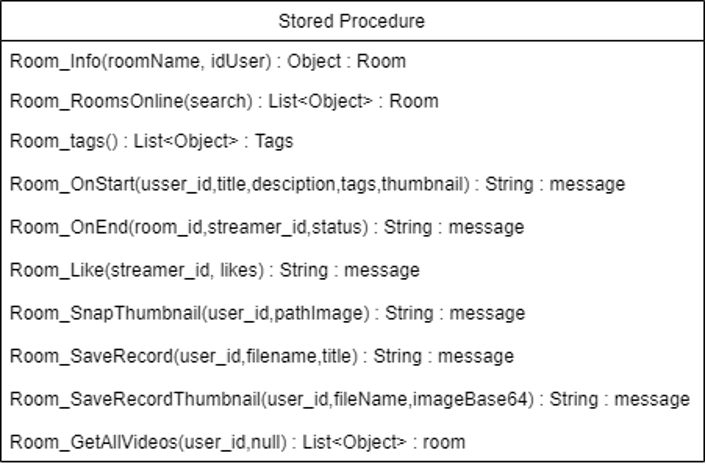
\includegraphics[width=17cm]{{./imgs/diagrams/stream_procedure}}
\end{center}

\begin{center}
\begin{longtabu} to \textwidth {| m{3cm} | m{5cm} | m{4cm} | m{4cm} |}
\caption{Các trường} \\
   \hline \textbf{Tên}  & \textbf{Mô tả} & \textbf{Input} & \textbf{Output}  \\ \hline
   \endfirsthead
   \hline \textbf{Tên}  & \textbf{Mô tả} & \textbf{Input} & \textbf{Output}  \\ \hline
   \endhead
      Info & Lấy thông tin Room  & roomName: tên room, idUser: mã user id & Thông tin phòng
      \\ \hline
      RoomOnline & Tìm kiếm Room  & Search: tên room cần tìm & Danh sách phòng đang online
      \\ \hline
      Tags & Lấy danh sách các tags &  & Danh sách tags
      \\ \hline
      OnStart & Tạo phòng và bắt đầu tạo video  & UserId: mã id của user, Title: chủ đề video, Description: mô tả về video, Tags: tên tags, Thumbnail: ảnh đại diên
 & Thông tin live stream
      \\ \hline
      OnEnd & Kết thúc video & RoomId: mã phòng, StreamerId: mã tài khoản, Status: tình trạng & Thông tin dừng live stream
      \\ \hline
      Like & Thực hiện like video & StreamerId: mã tài khoản, Likes: 1 - 0 & Trạng thái
      \\ \hline
      SnapThumbnail & Snap hình ảnh& UserId: mã tài khoản, pathImage: ảnh & Trạng thái
      \\ \hline
      SaveRecord & Lưu video & UserId: mã tài khoản, fileName: đường dẫn video, title: tên chủ đề & Trạng thái
      \\ \hline
      SaveRecord Thumbnail & Lưu ảnh video & UserId: mã tài khoản, fileName: file video, imageBase64: ảnh & Trạng thái
      \\ \hline
      GetAllVideos & Lấy thông tin tất cả video & UserId: mã tài khoản & Danh sách video
      \\ \hline
\end{longtabu}
\end{center}


\begin{center}
	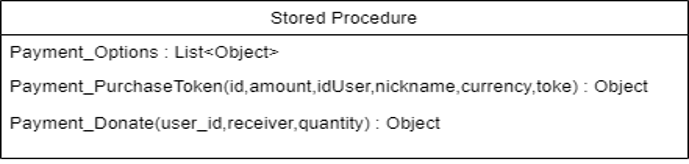
\includegraphics[width=17cm]{{./imgs/diagrams/payment_procedure}}
\end{center}

\begin{center}
\begin{longtabu} to \textwidth {| m{3cm} | m{5cm} | m{4cm} | m{4cm} |}
\caption{Các trường} \\
   \hline \textbf{Tên}  & \textbf{Mô tả} & \textbf{Input} & \textbf{Output}  \\ \hline
   \endfirsthead
   \hline \textbf{Tên}  & \textbf{Mô tả} & \textbf{Input} & \textbf{Output}  \\ \hline
   \endhead
      Option & Danh sách tiền tệ  &  & Danh sách lựa chọn token
      \\ \hline
      PurchaseToken & Mua token & Id: mã tài khoản, Amount: số tiền, idUser: mã id user, nickname: tên nickname, currency: tỉ lệ đổi, toke: số lượng token
 & Thông tin mua token
      \\ \hline
      Donate & Donate token & Userid: mã id user, Receiver: người nhận, Quantity: số lượng
 & Thông tin donate 
      \\ \hline
\end{longtabu}
\end{center}


\begin{center}
	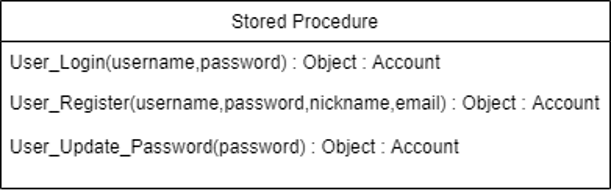
\includegraphics[width=17cm]{{./imgs/diagrams/credential_procedure}}
\end{center}

\begin{center}
\begin{longtabu} to \textwidth {| m{3cm} | m{5cm} | m{4cm} | m{4cm} |}
\caption{Các trường} \\
   \hline \textbf{Tên}  & \textbf{Mô tả} & \textbf{Input} & \textbf{Output}  \\ \hline
   \endfirsthead
   \hline \textbf{Tên}  & \textbf{Mô tả} & \textbf{Input} & \textbf{Output}  \\ \hline
   \endhead
      Login & Đăng nhập tài khoản  & Username: tên đăng nhập, Password: mật khẩu
 & Trạng thái đăng nhập
      \\ \hline
      Register & Đăng ký tài khoản  & Username: tên đăng nhập, Password: mật khẩu, Nickname: tên nickname, Emai: địa chỉ email & Thông tin đăng ký
      \\ \hline
      UpdatePassword & Đổi mật khẩu & Password: mật khẩu & Trạng thái cập nhật
      \\ \hline
\end{longtabu}
\end{center}















\chapter{THỰC HIỆN}
\section{Giao Diện}


\begin{center}
\begin{figure}[H]
\begin{tabular}{cc}
  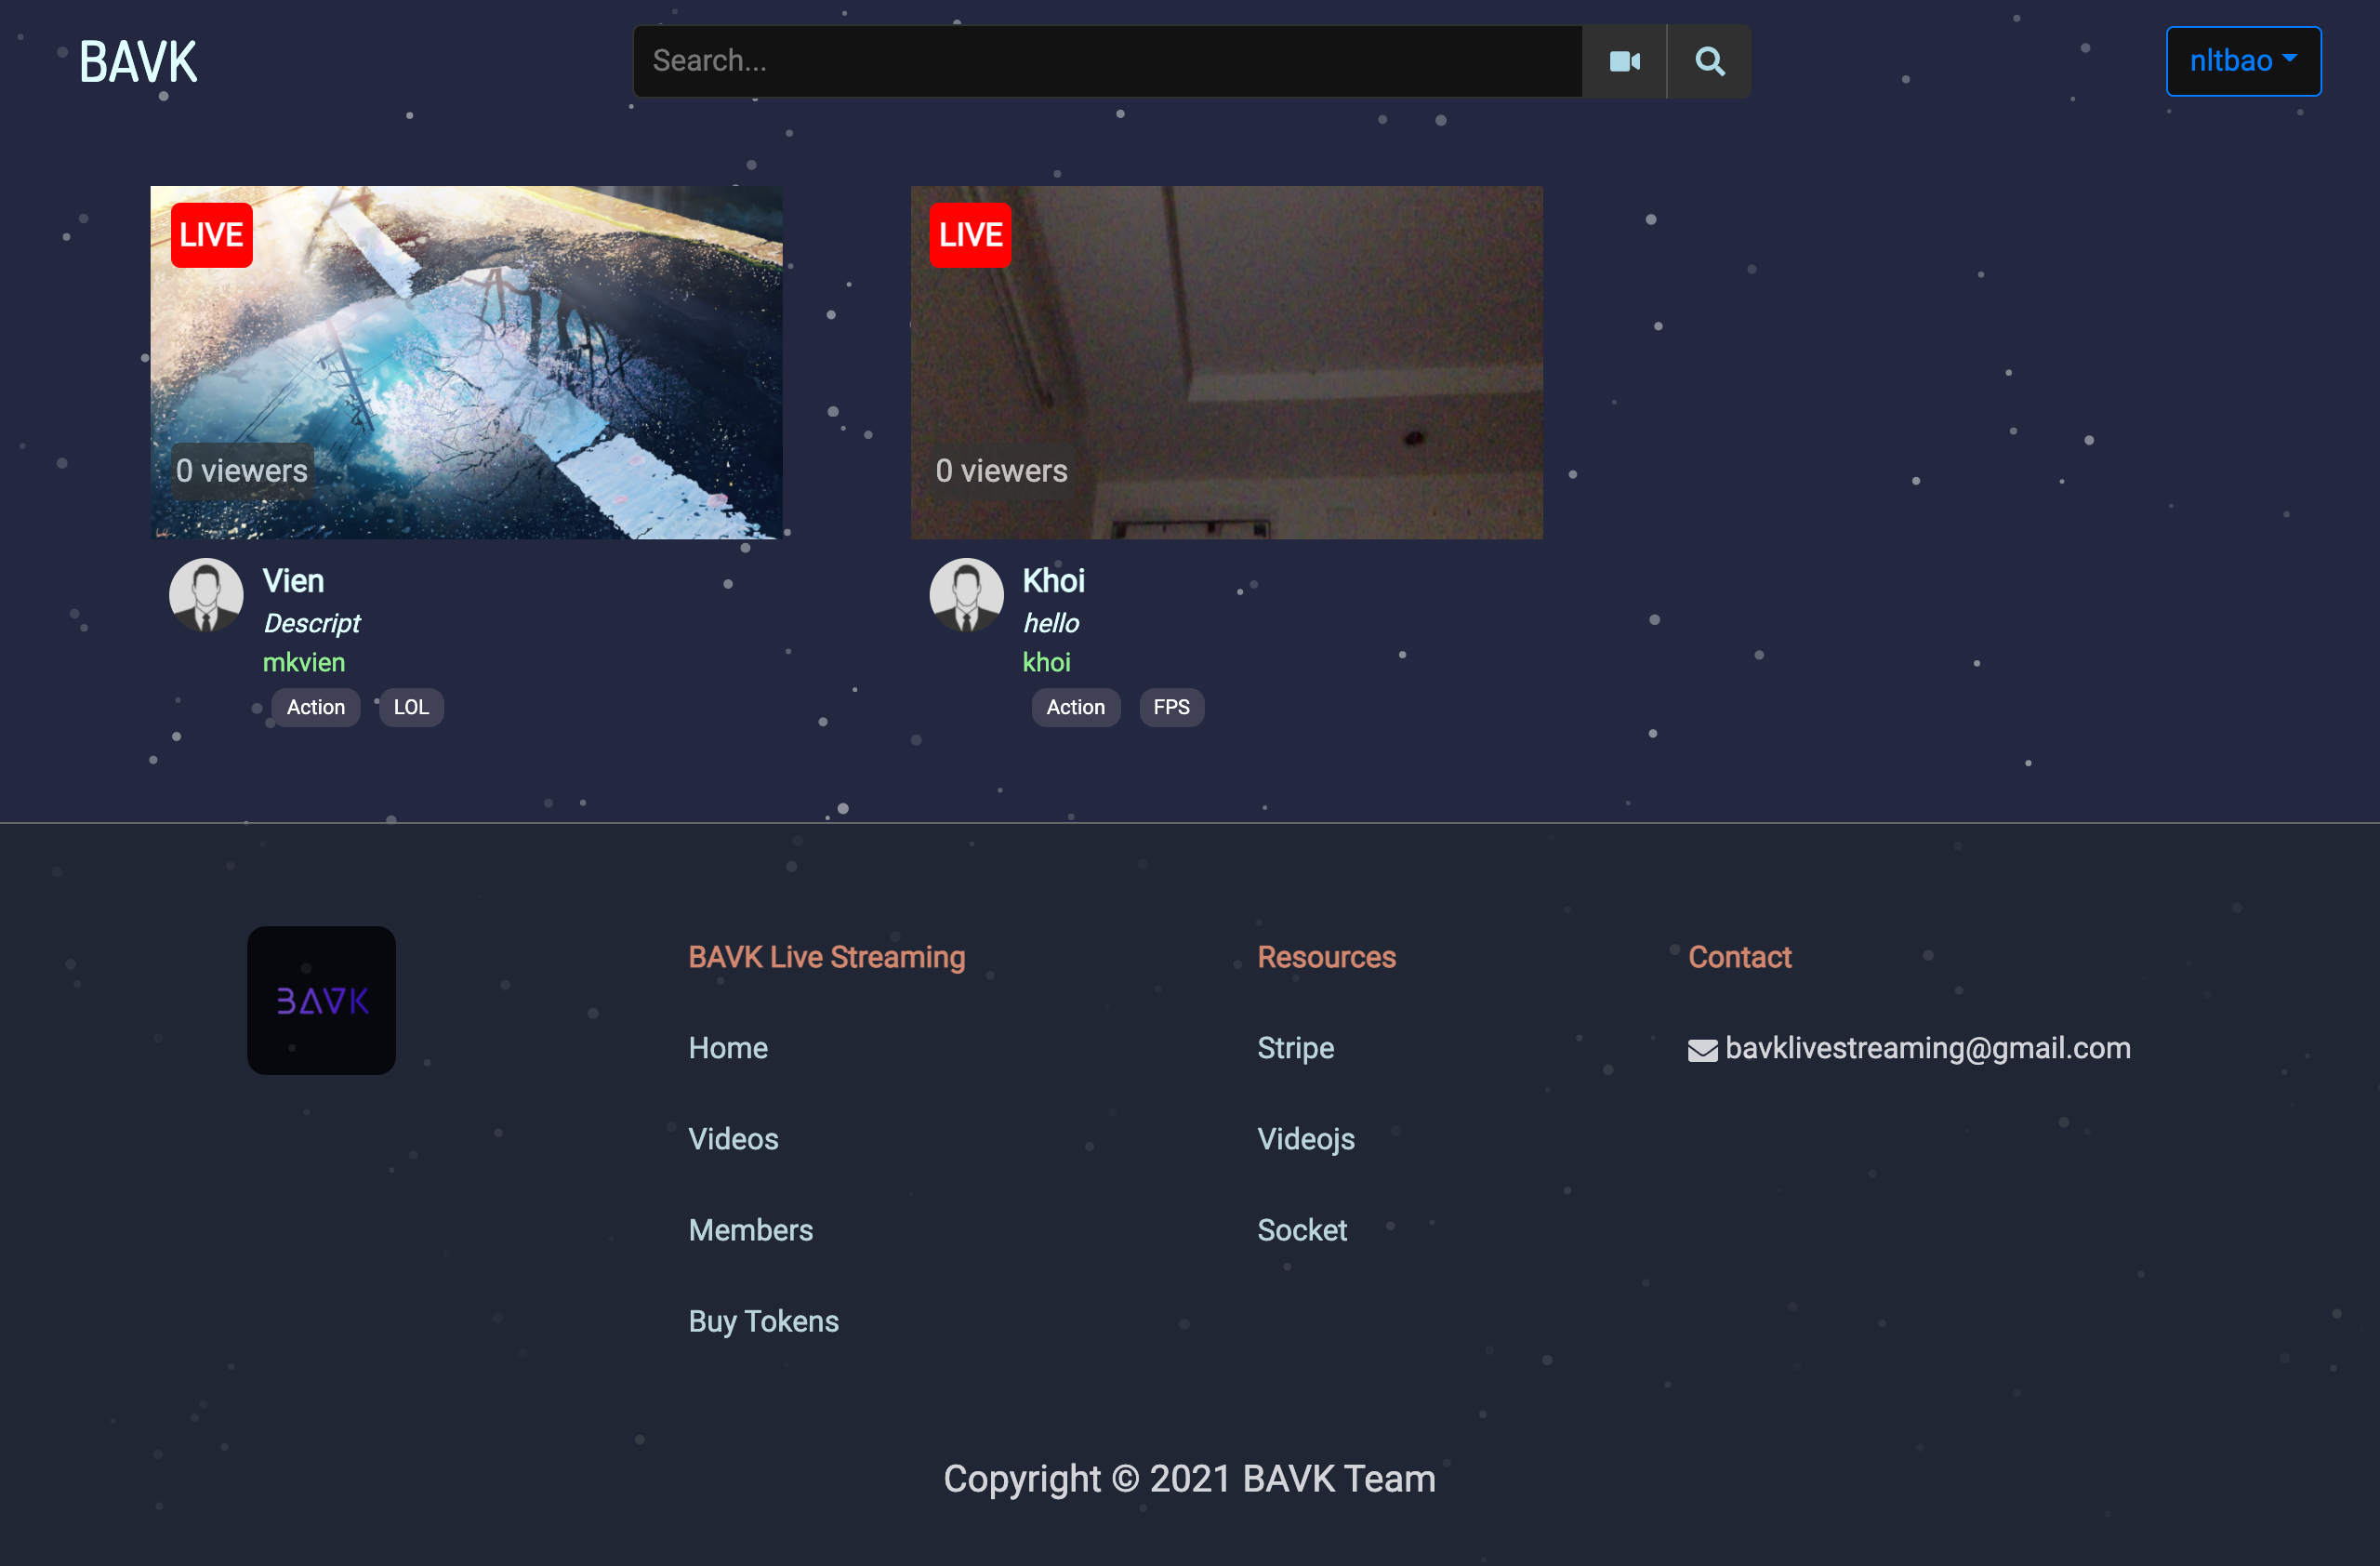
\includegraphics[width=8.5cm, height=8cm]{./imgs/layouts/home} &   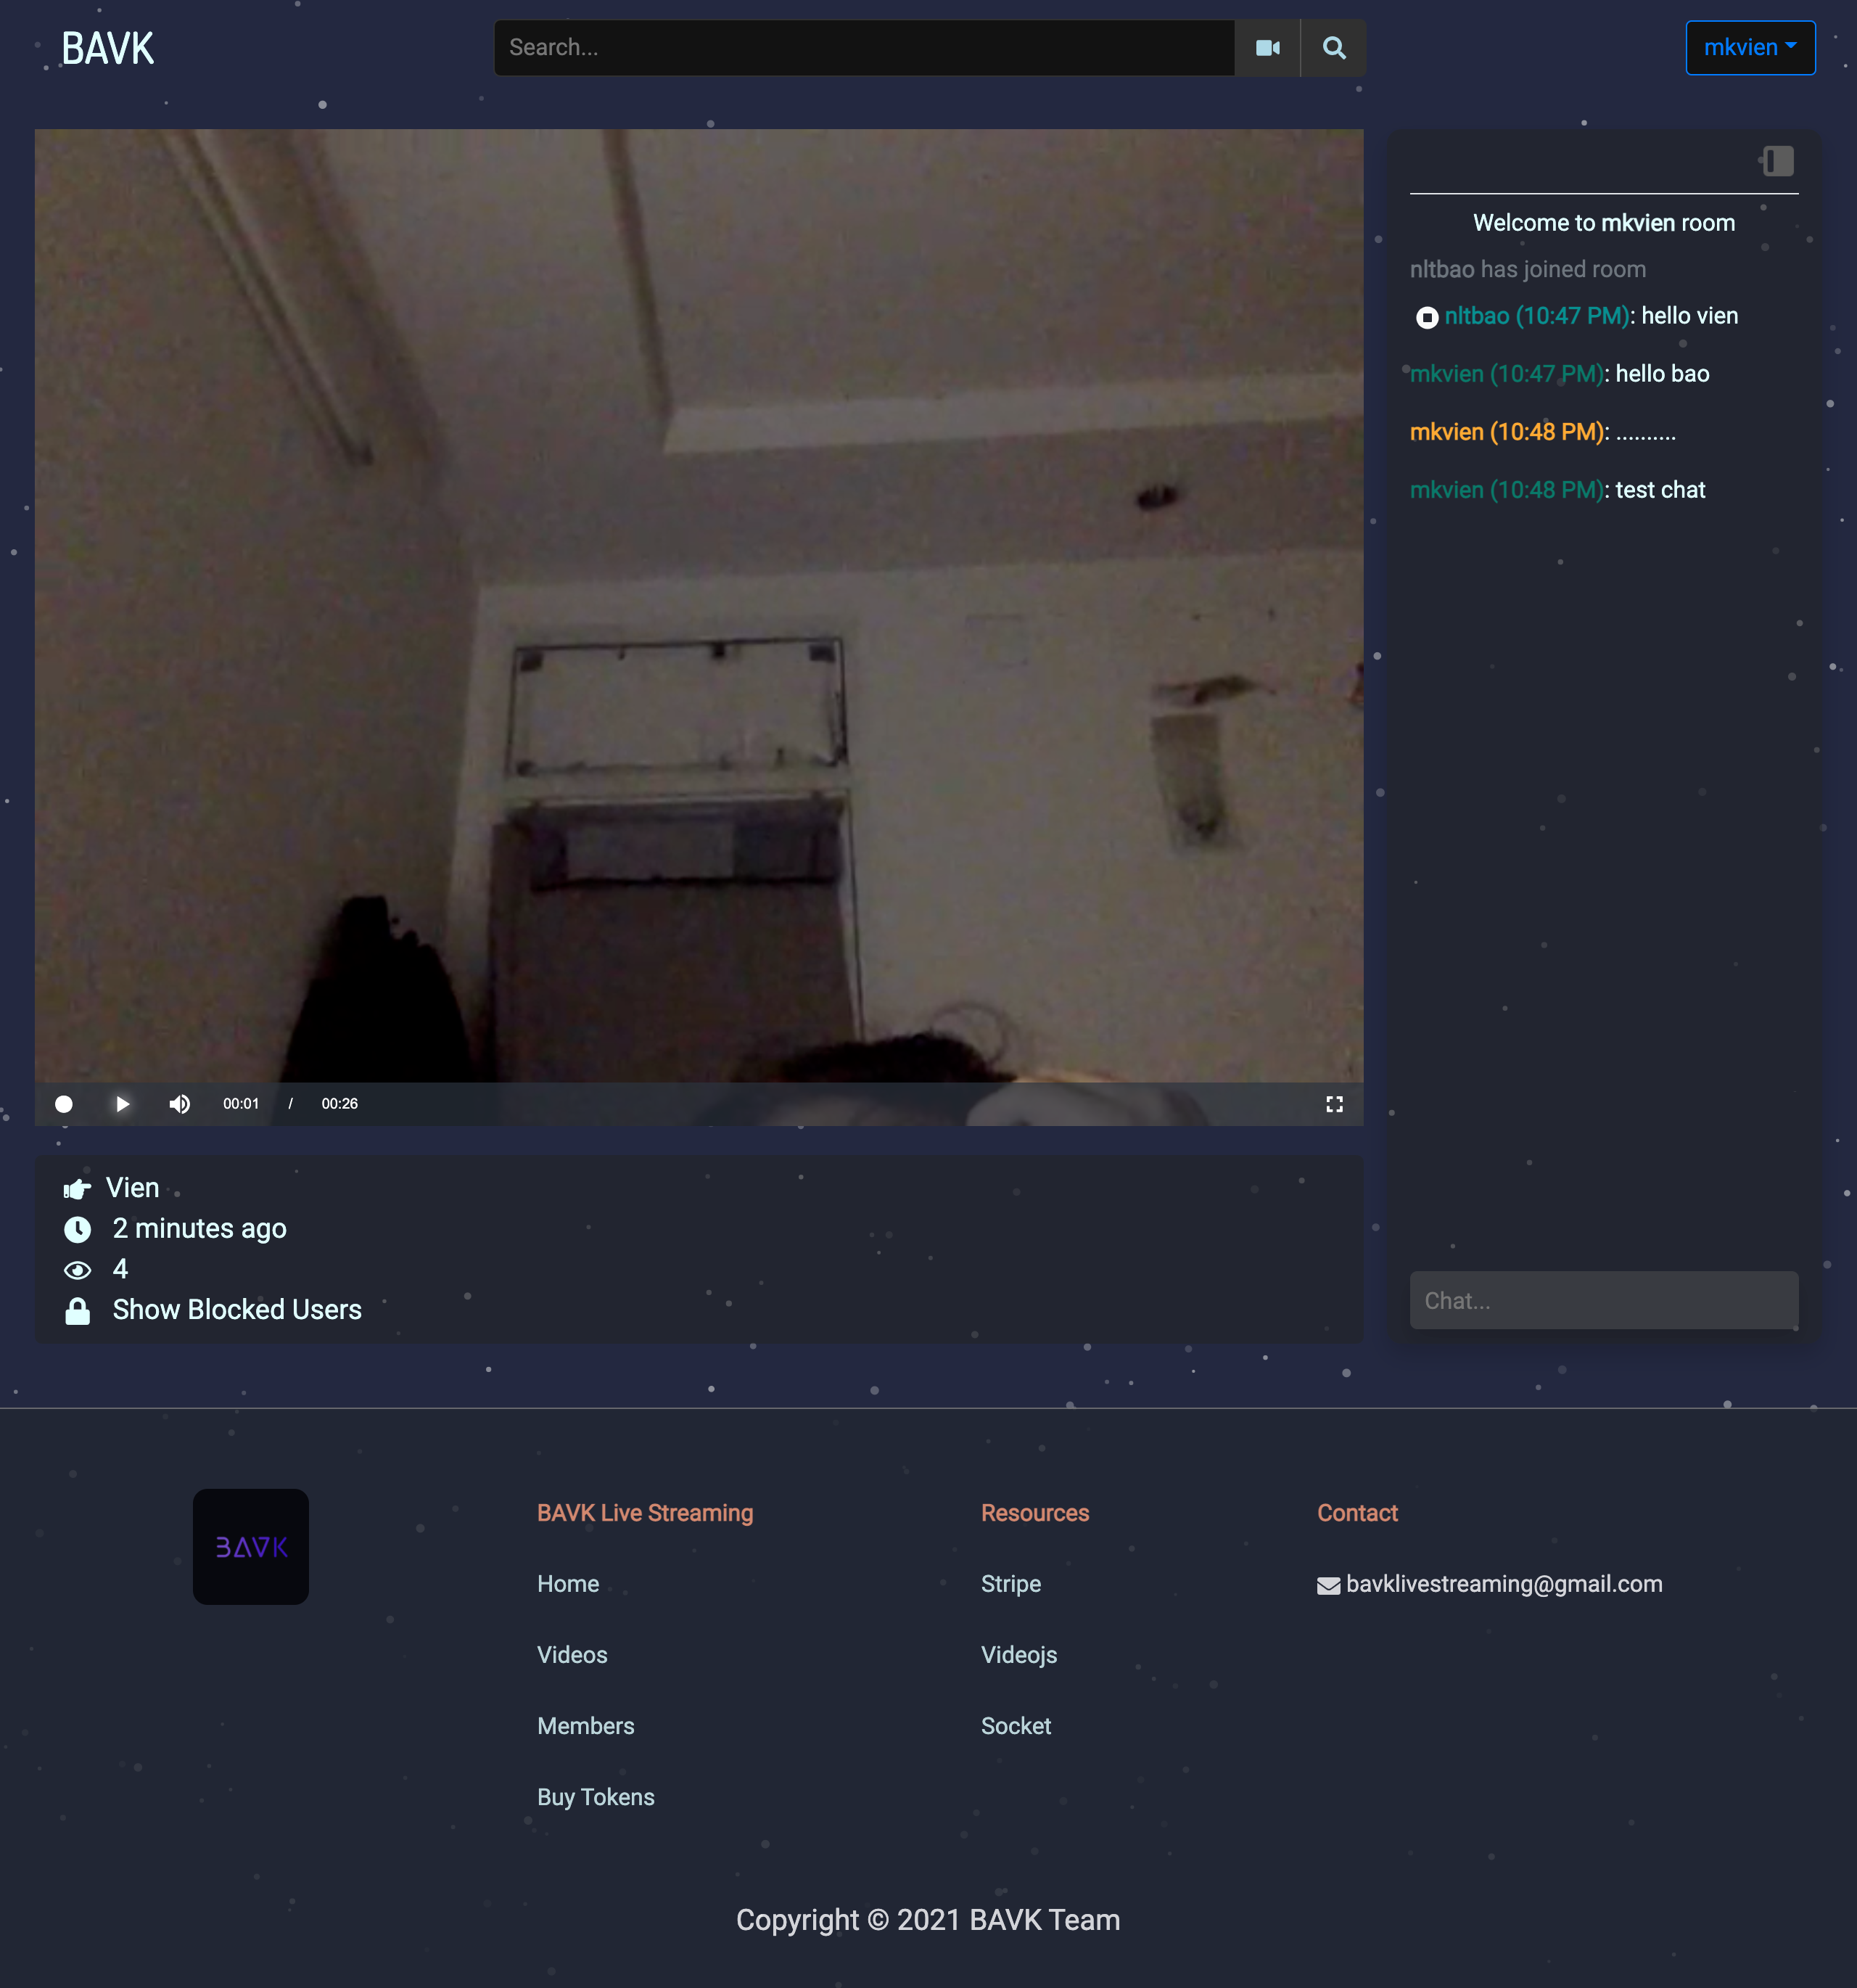
\includegraphics[width=8.5cm, height=8cm]{./imgs/layouts/streamer} \\
Trang chủ & Trang Streamer \\[6pt]
\end{tabular}
\end{figure}
\end{center}

\begin{center}
\begin{figure}[H]
\begin{tabular}{cc}
  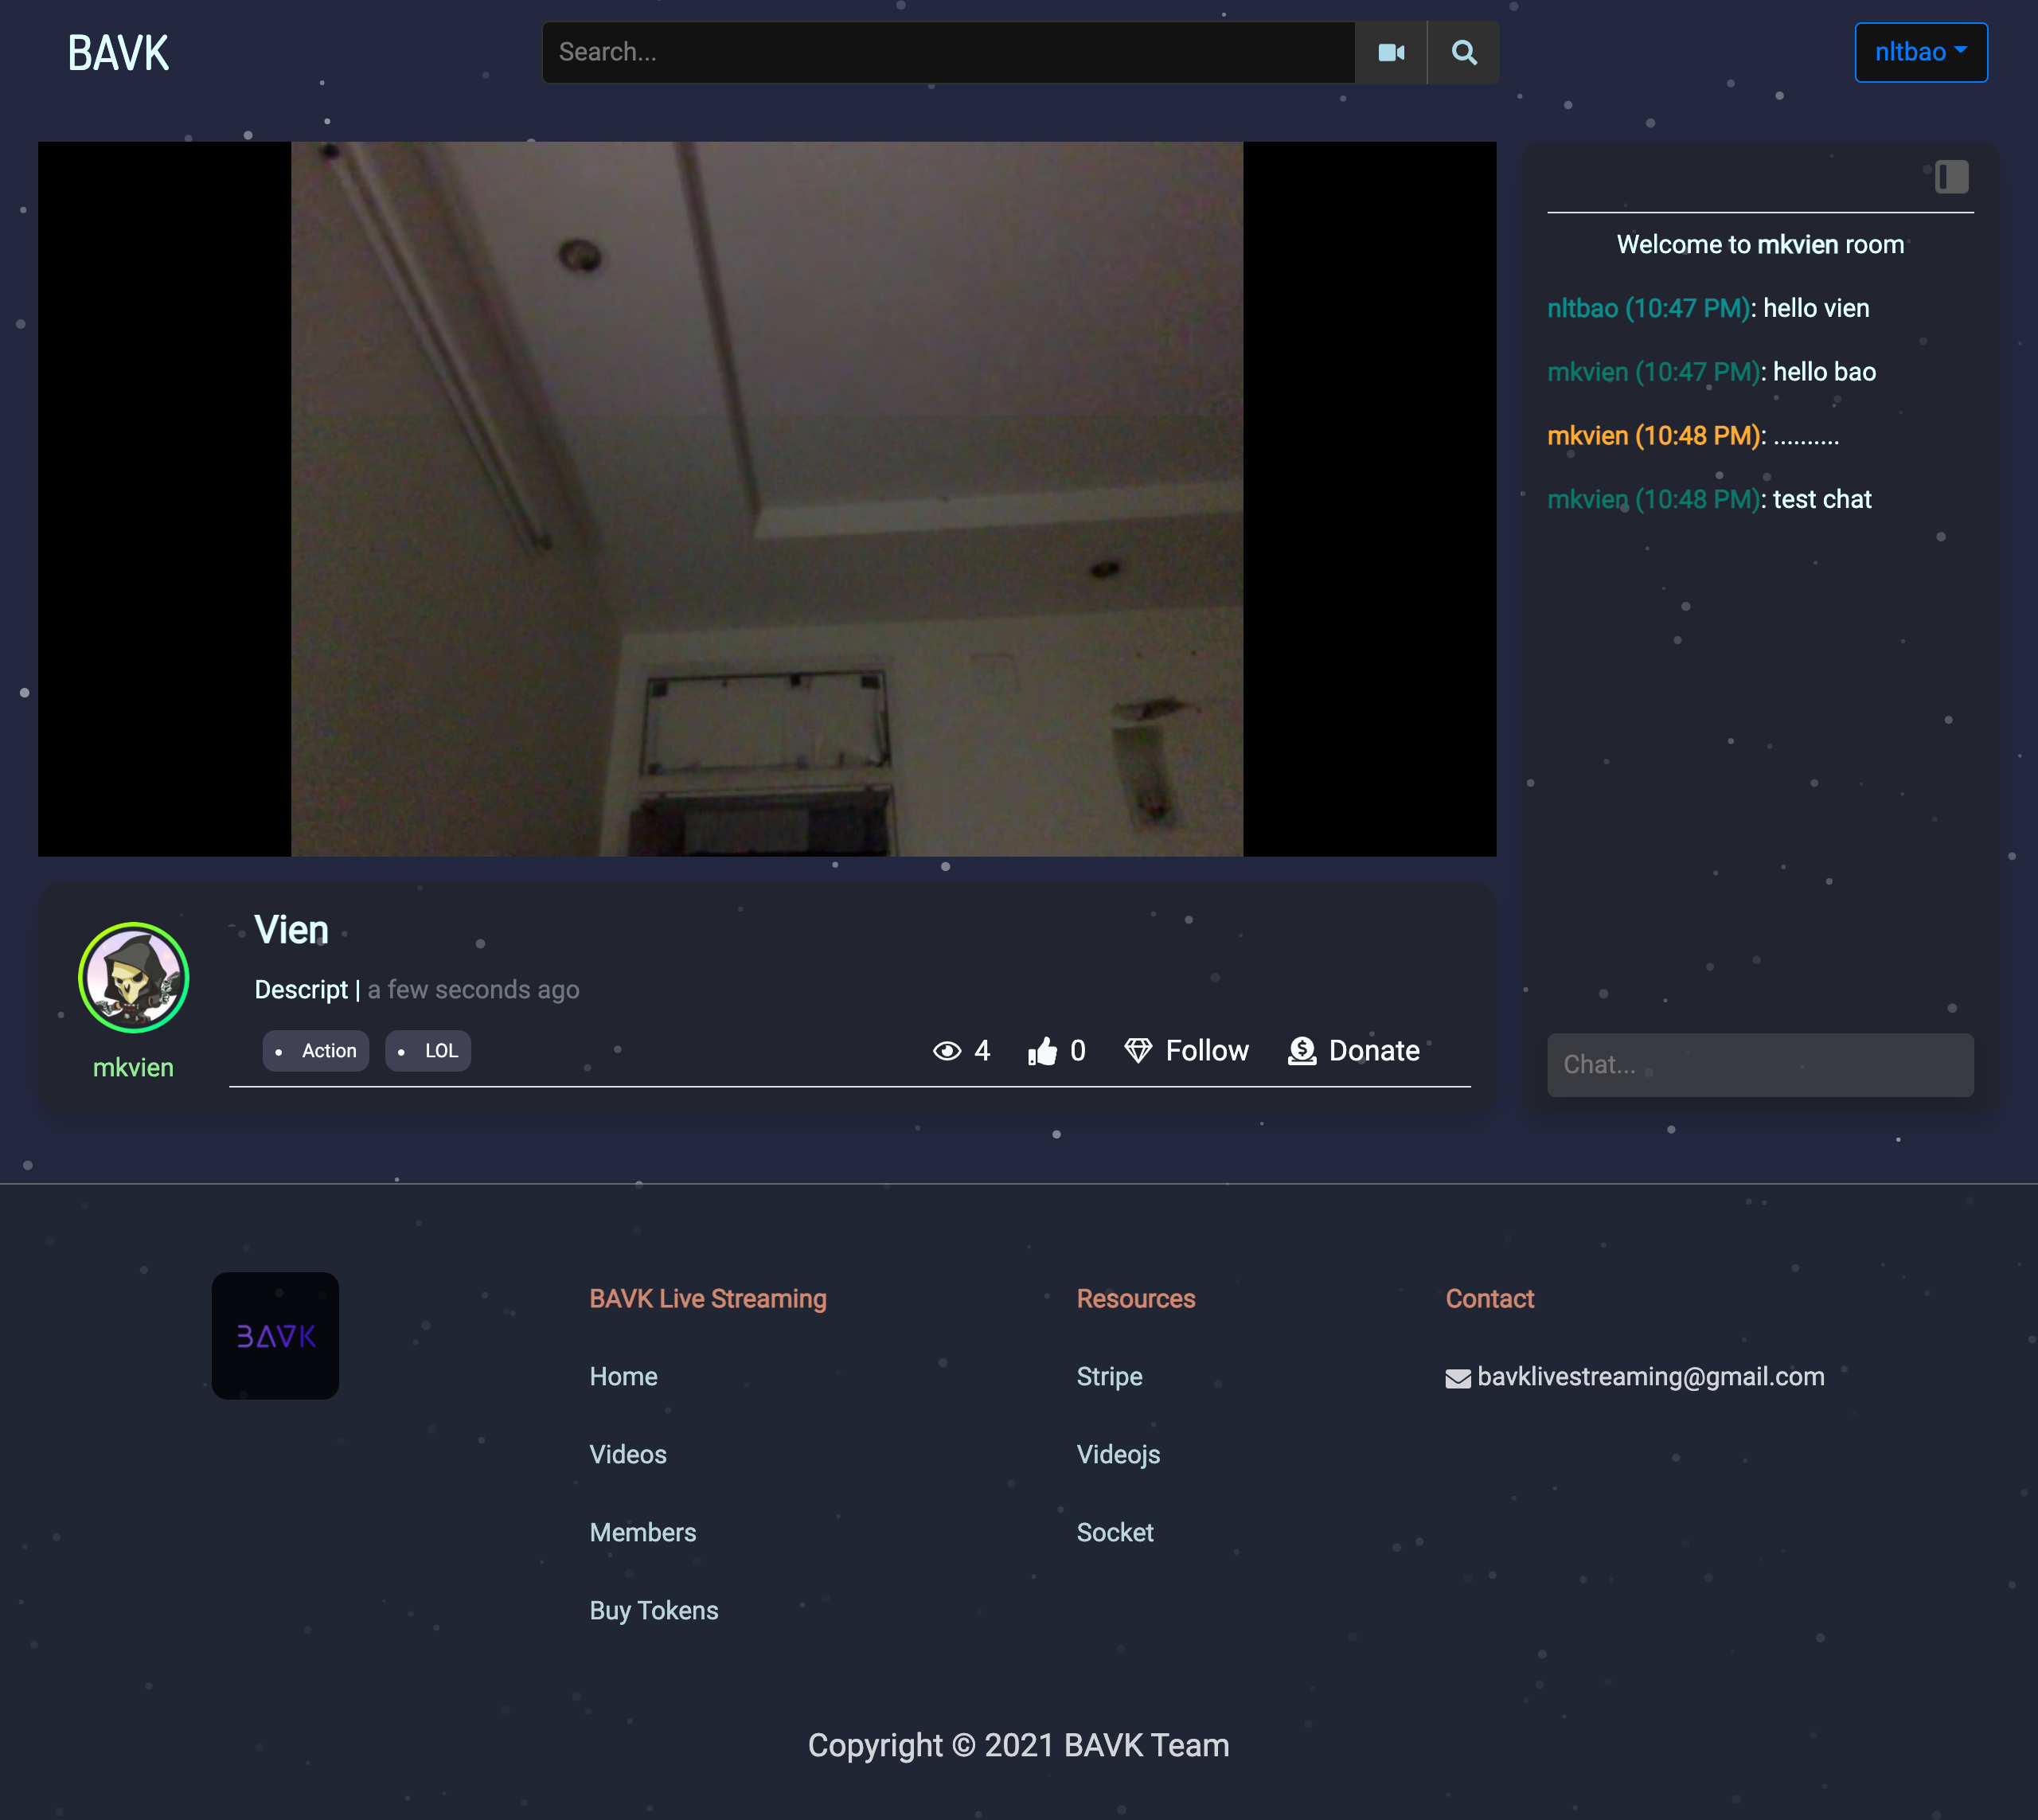
\includegraphics[width=8.5cm, height=8cm]{./imgs/layouts/viewer} &   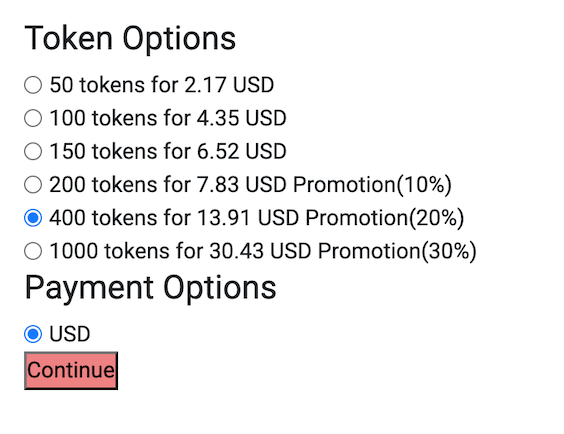
\includegraphics[width=8.5cm,height=8cm]{./imgs/layouts/option_buy} \\
Trang Viewer & Trang mua token \\[6pt]
\end{tabular}
\end{figure}
\end{center}

\begin{center}
\begin{figure}[H]
\begin{tabular}{cc}
  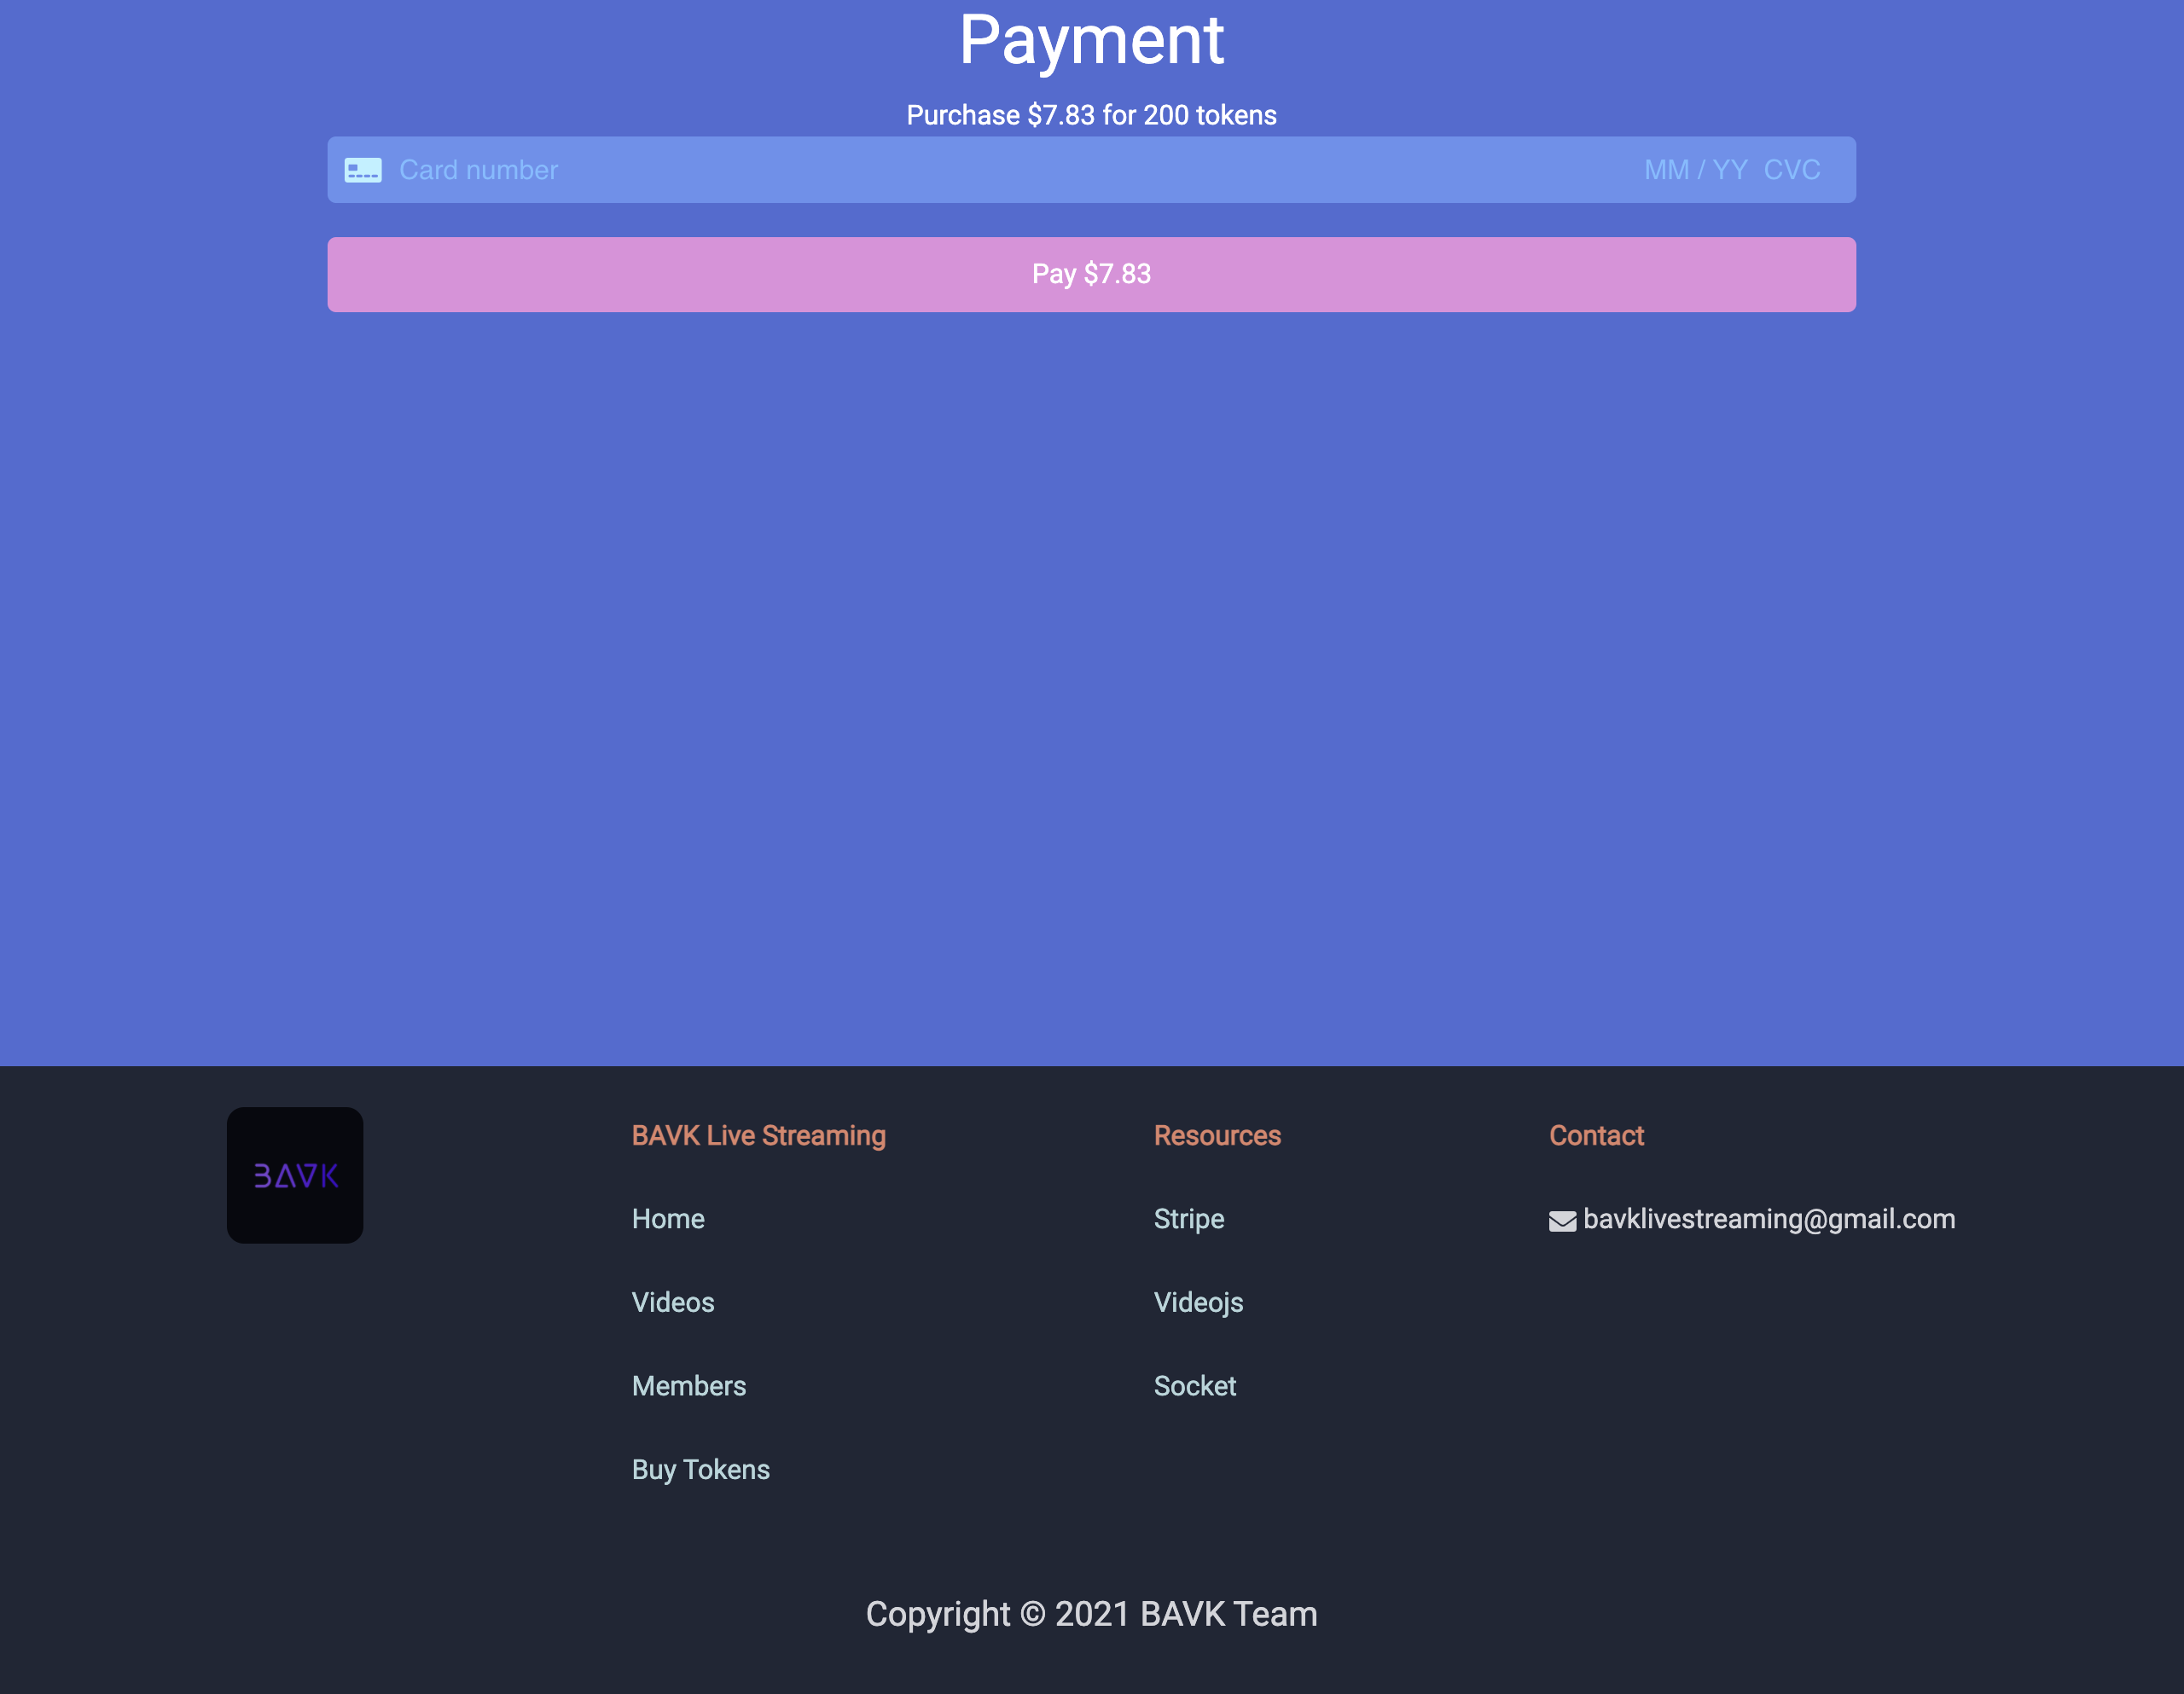
\includegraphics[width=8.5cm,height=8cm]{./imgs/layouts/proceed_to_payment} &   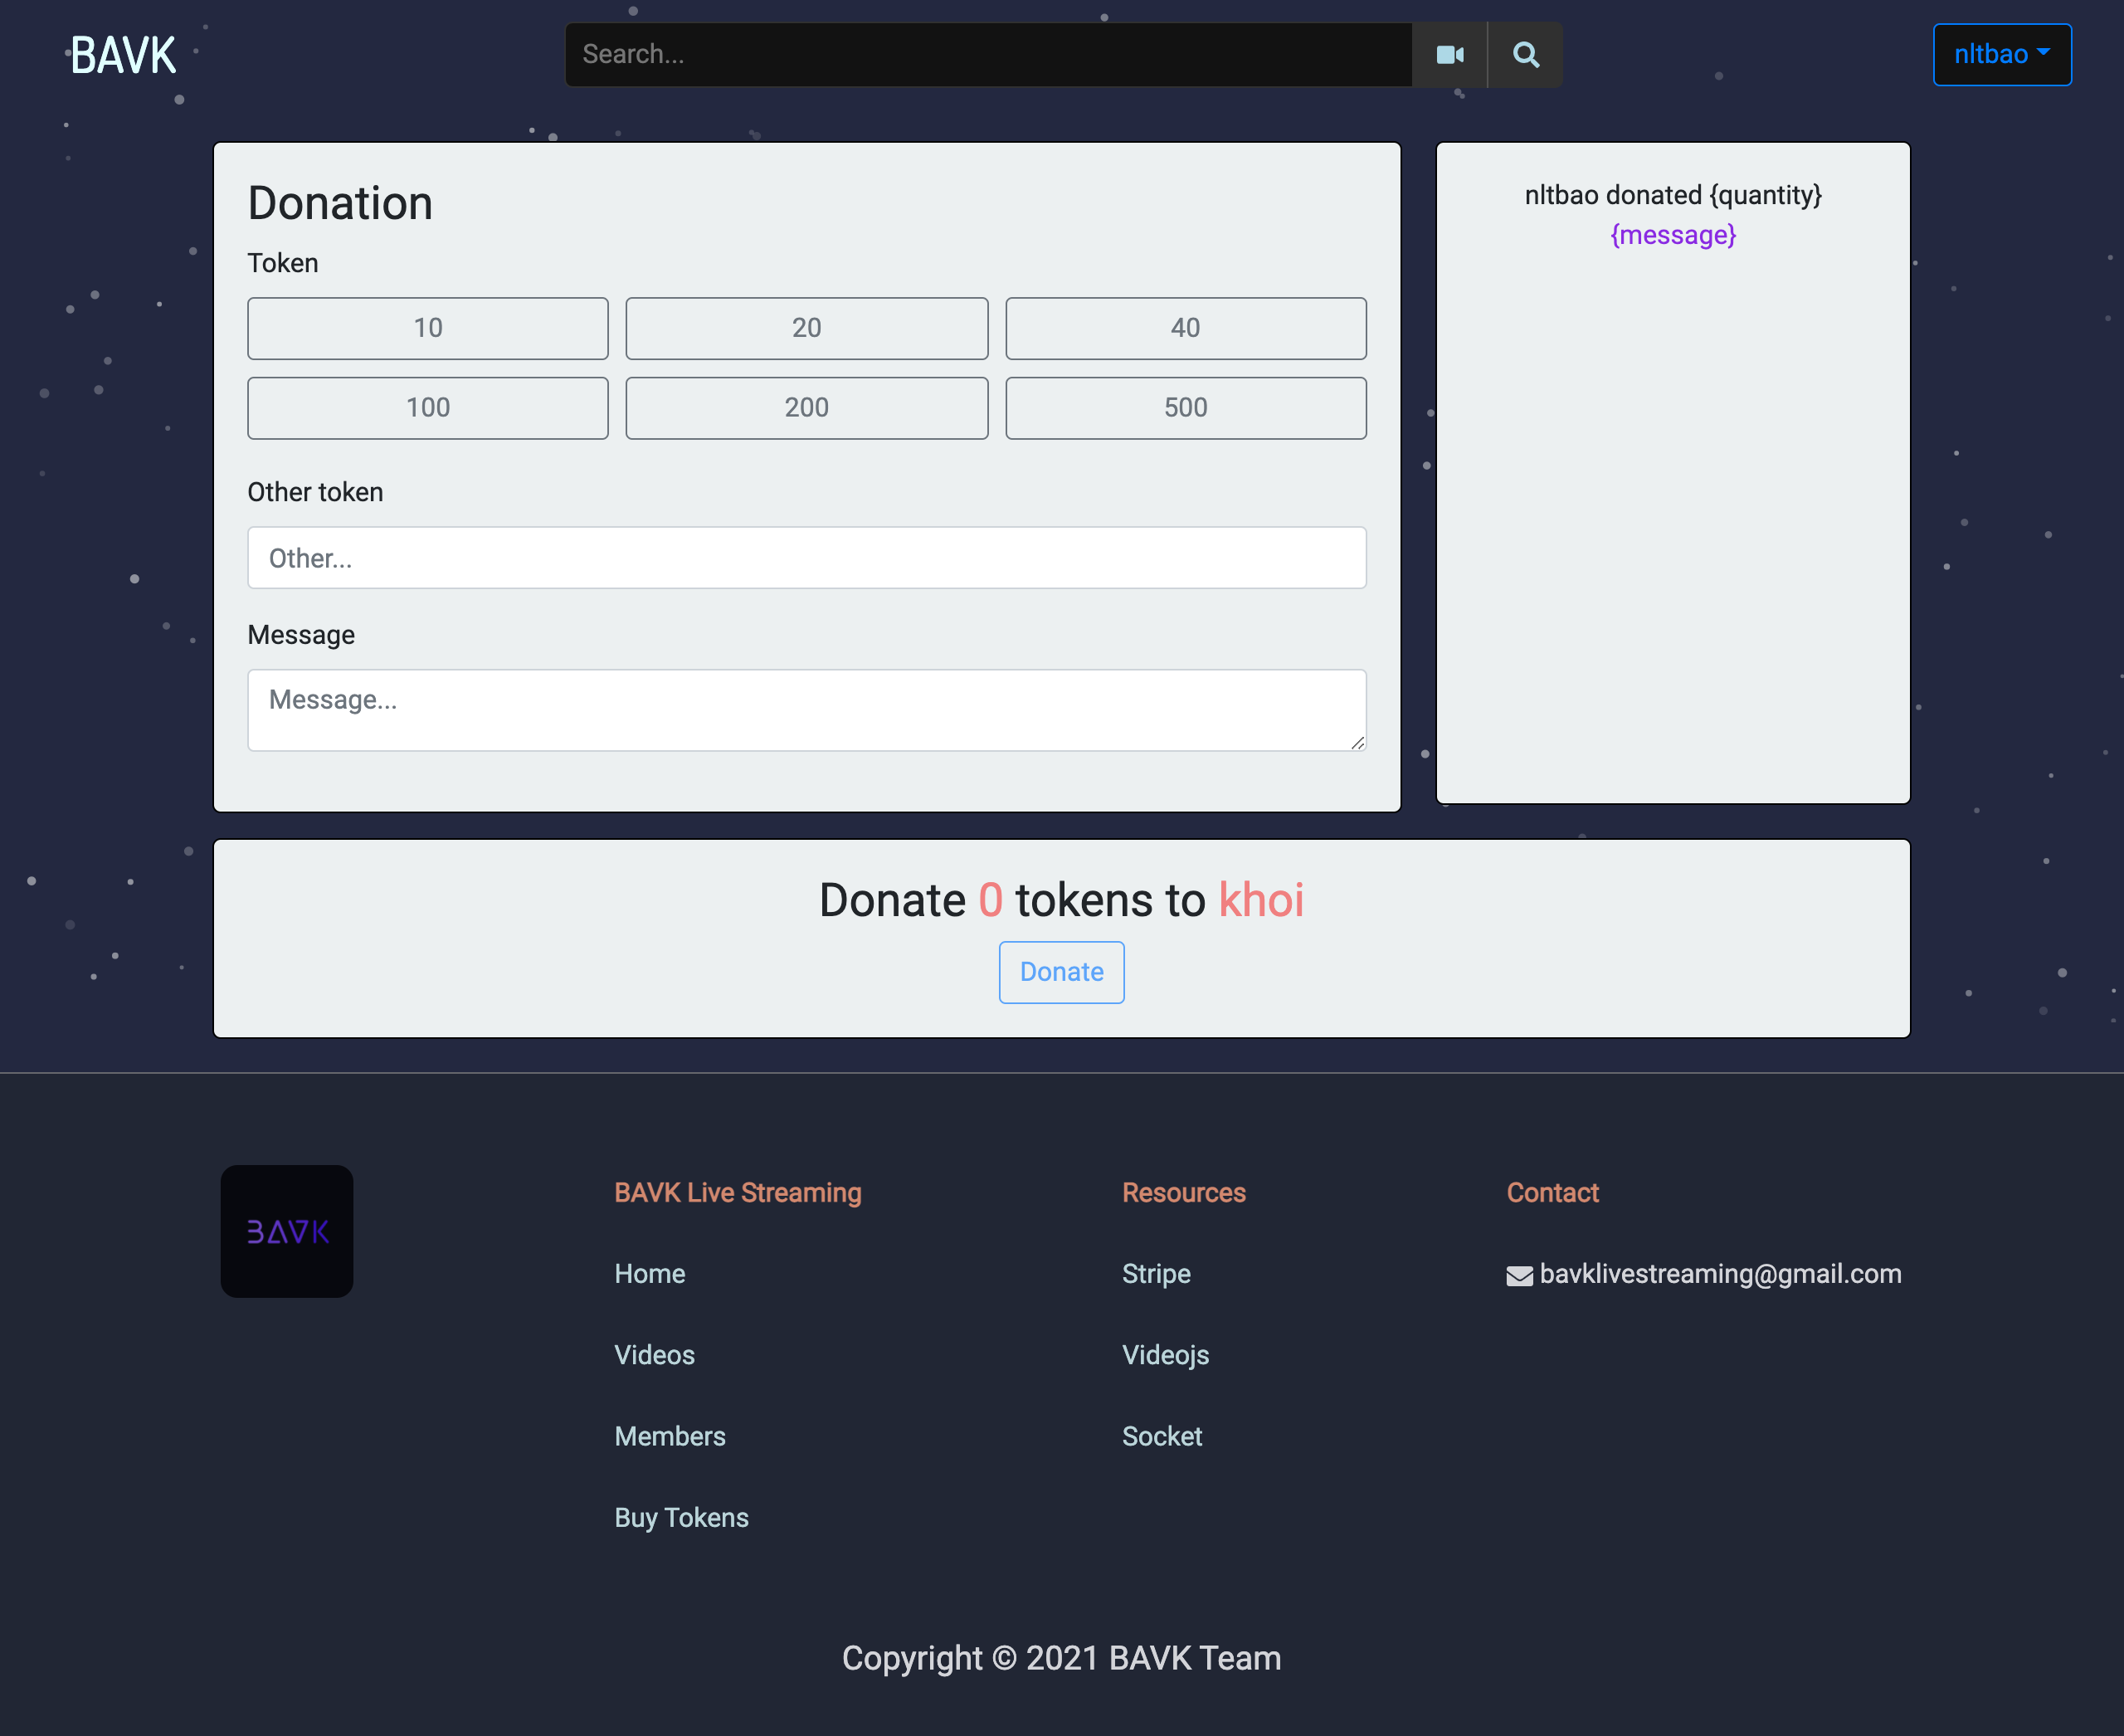
\includegraphics[width=8.5cm,height=8cm]{./imgs/layouts/donate} \\
Trang thanh toán & Trang donate \\[6pt]
\end{tabular}
\end{figure}
\end{center}

\begin{center}
\begin{figure}[H]
\begin{tabular}{cc}
  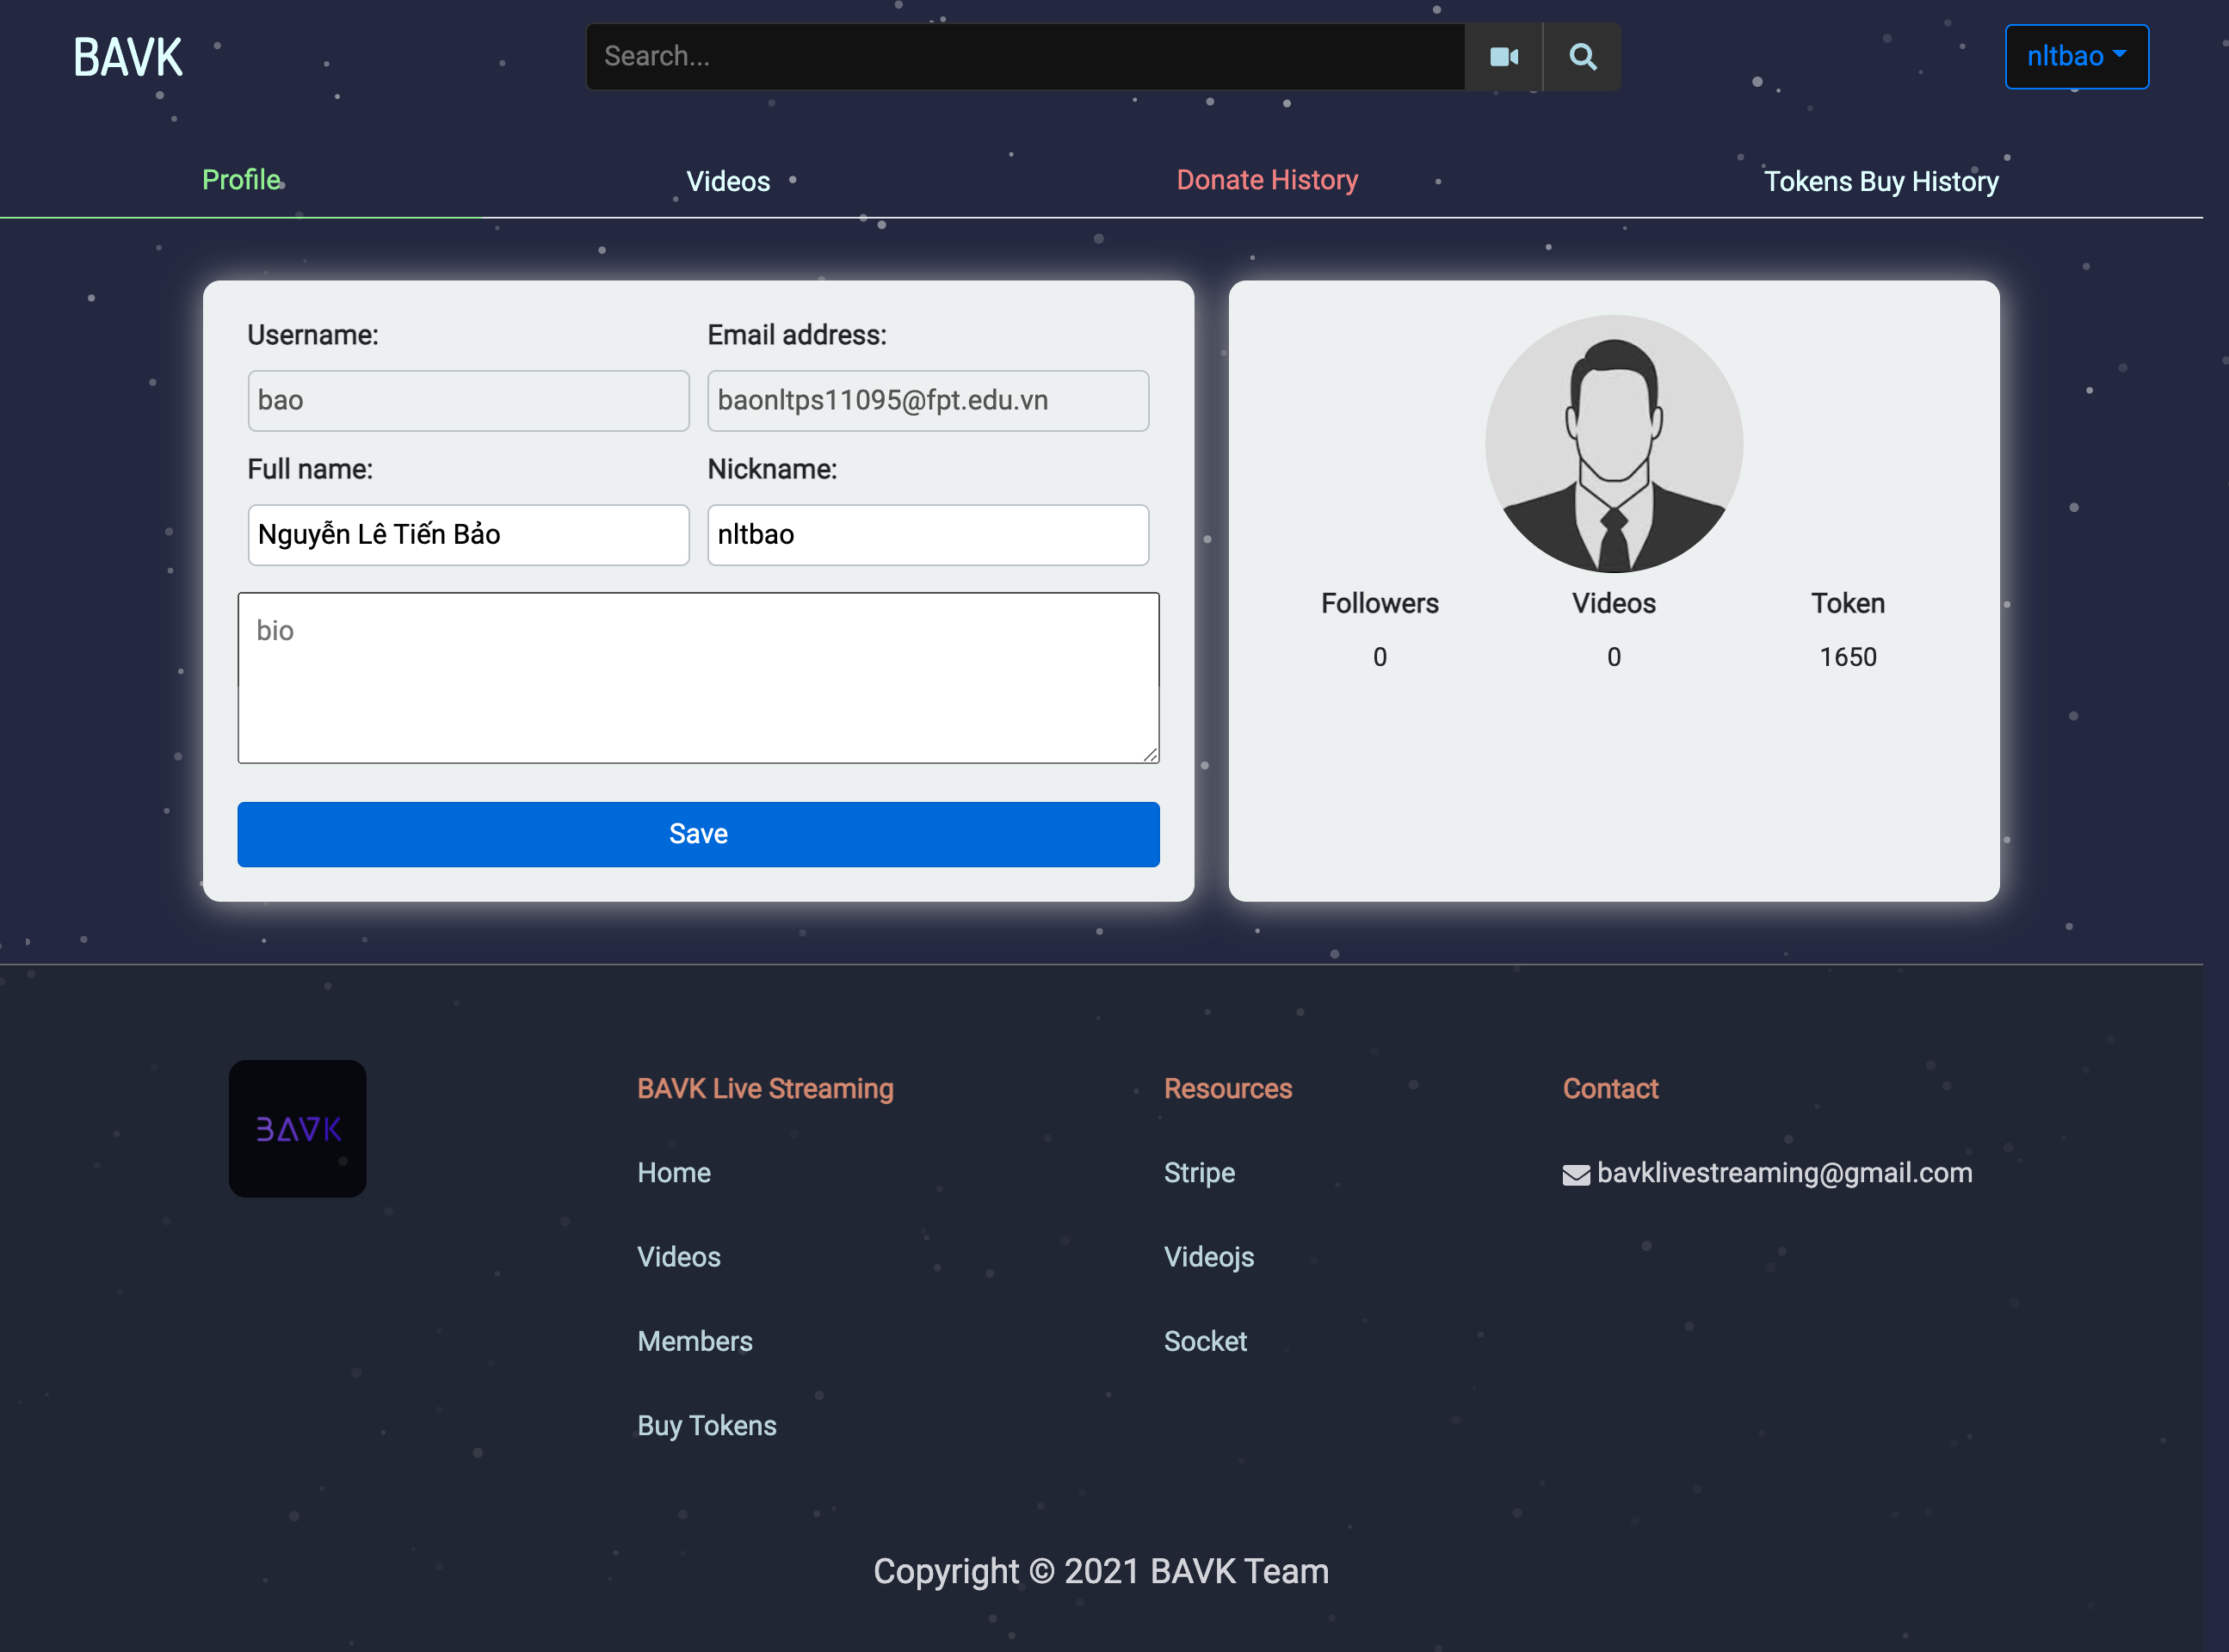
\includegraphics[width=8.5cm,height=8cm]{./imgs/layouts/profile} &   \includegraphics[width=8.5cm,height=8cm]{./imgs/layouts/history_donate} \\
Trang hồ sơ & Trang lịch sử donate \\[6pt]
\end{tabular}
\end{figure}
\end{center}

\begin{center}
\begin{figure}[H]
\begin{tabular}{cc}
  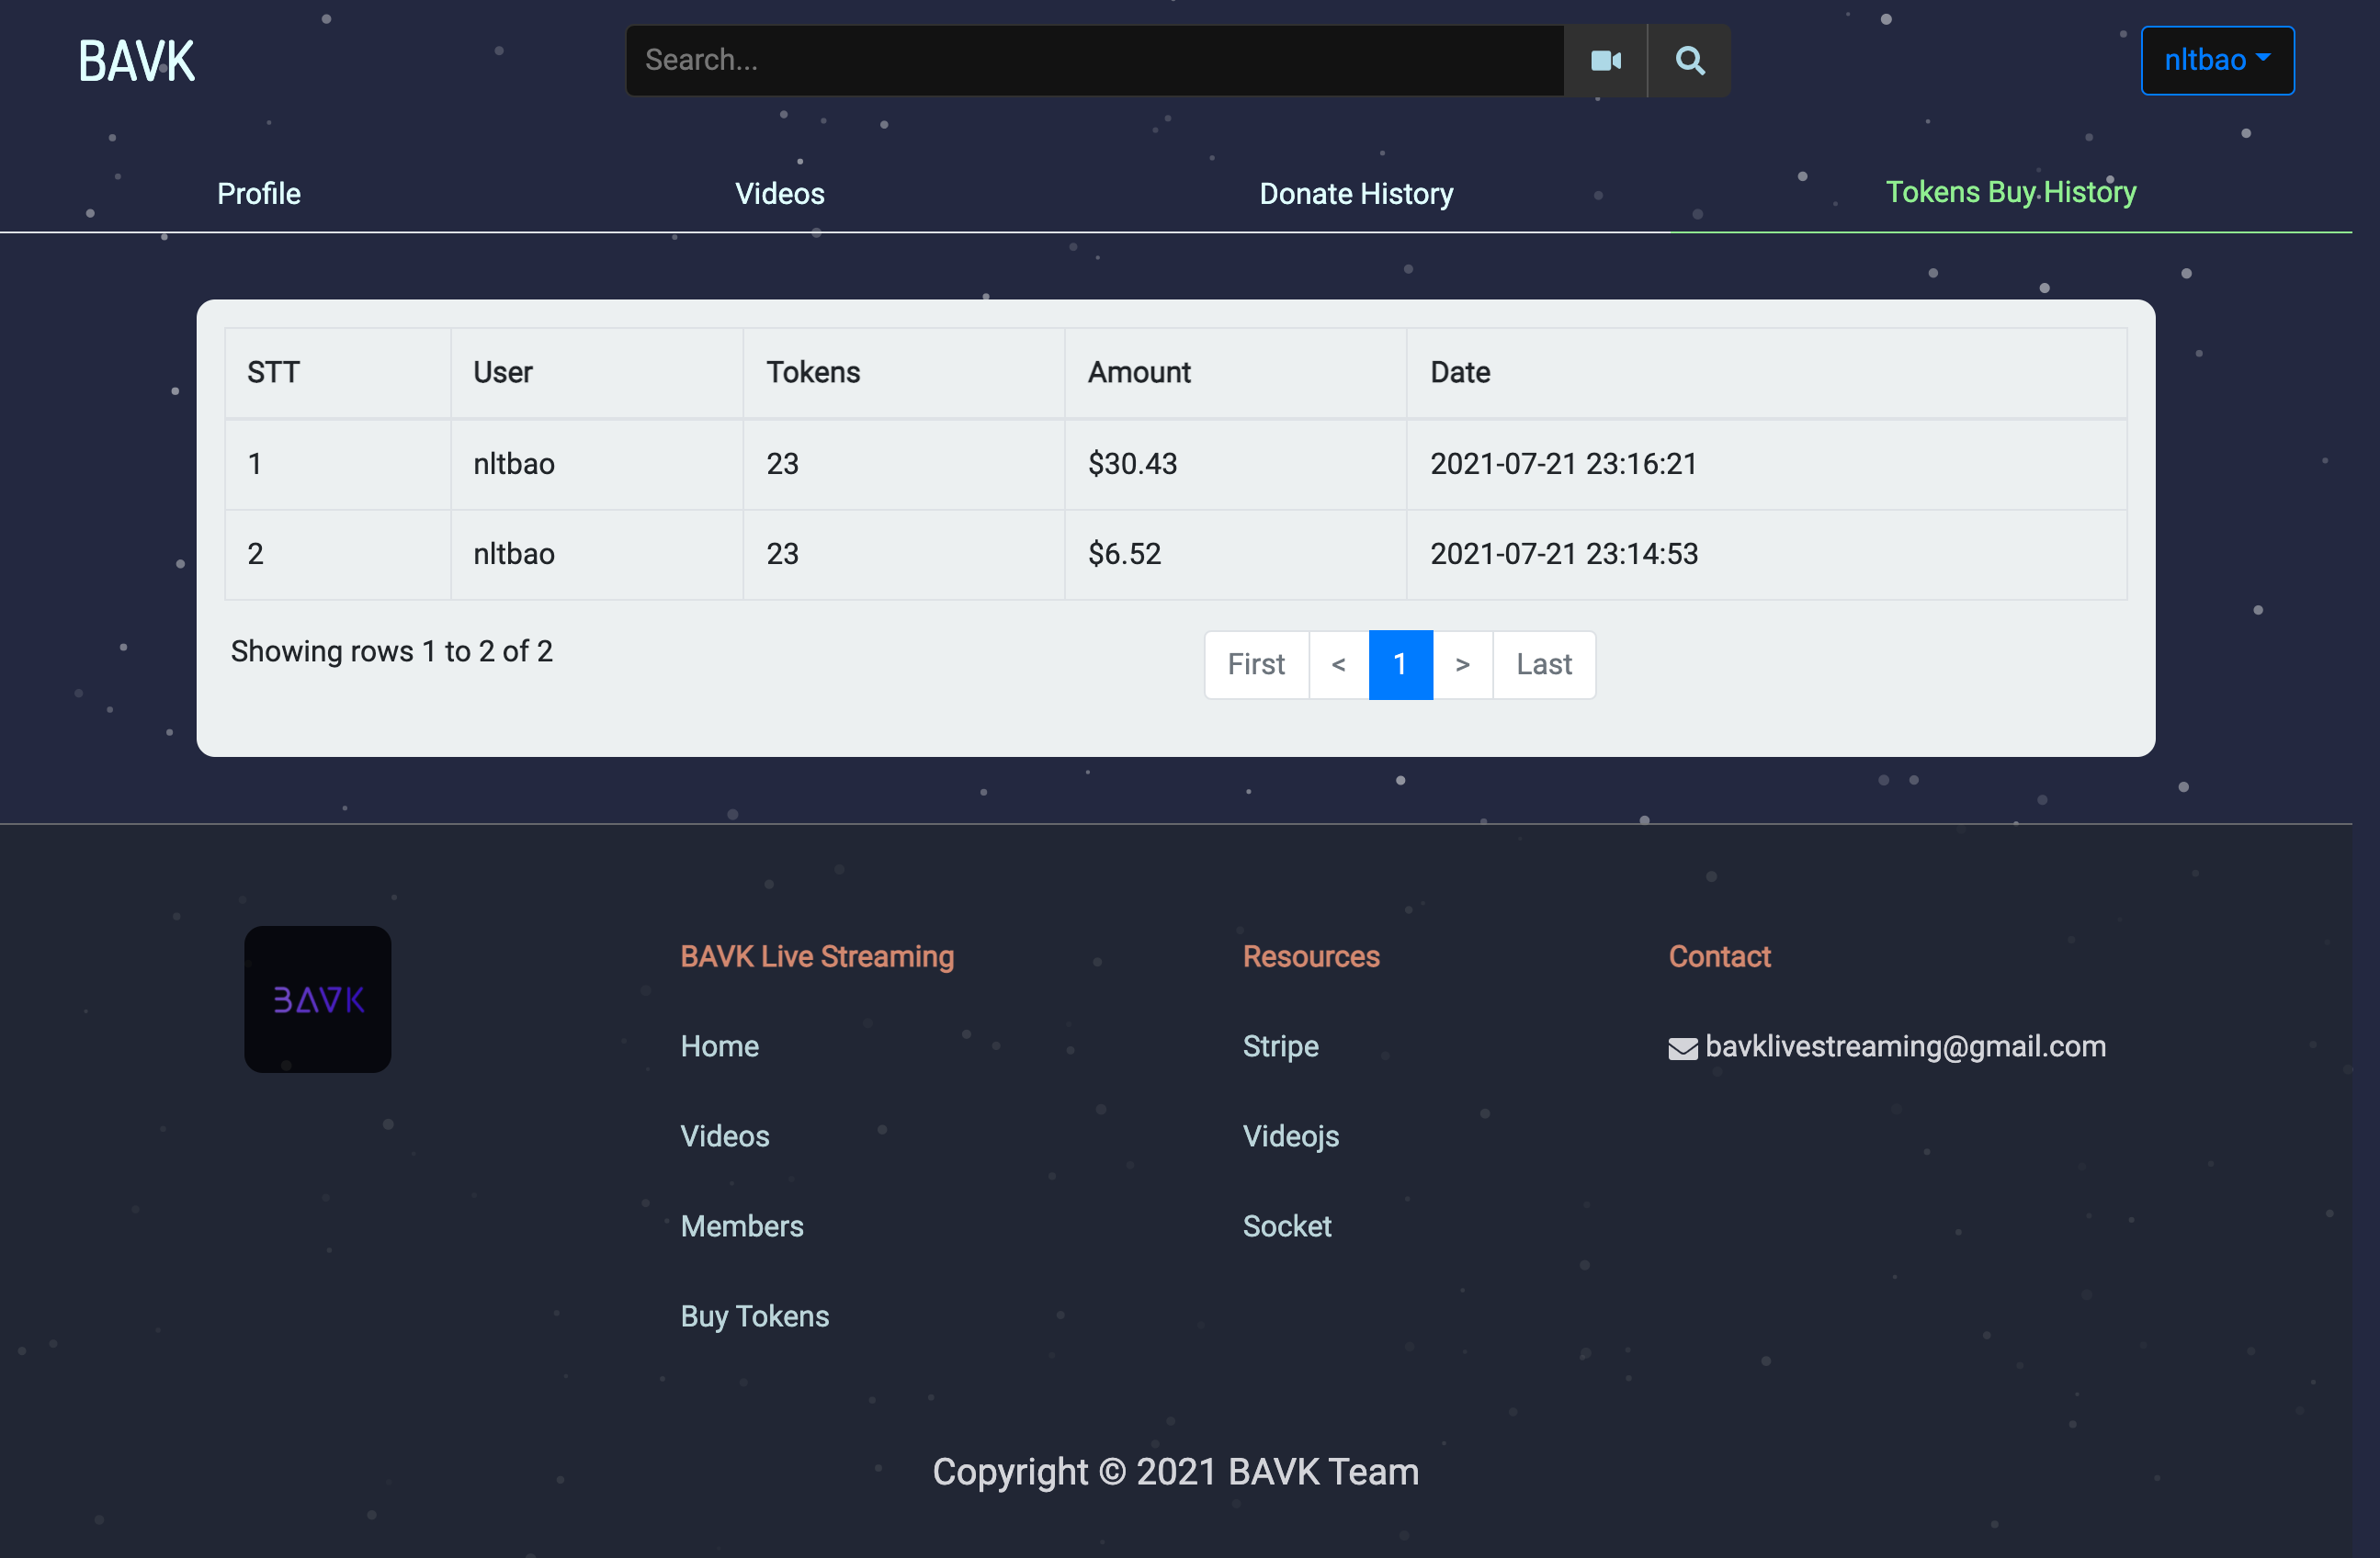
\includegraphics[width=8.5cm,height=8cm]{./imgs/layouts/history_tokens} &   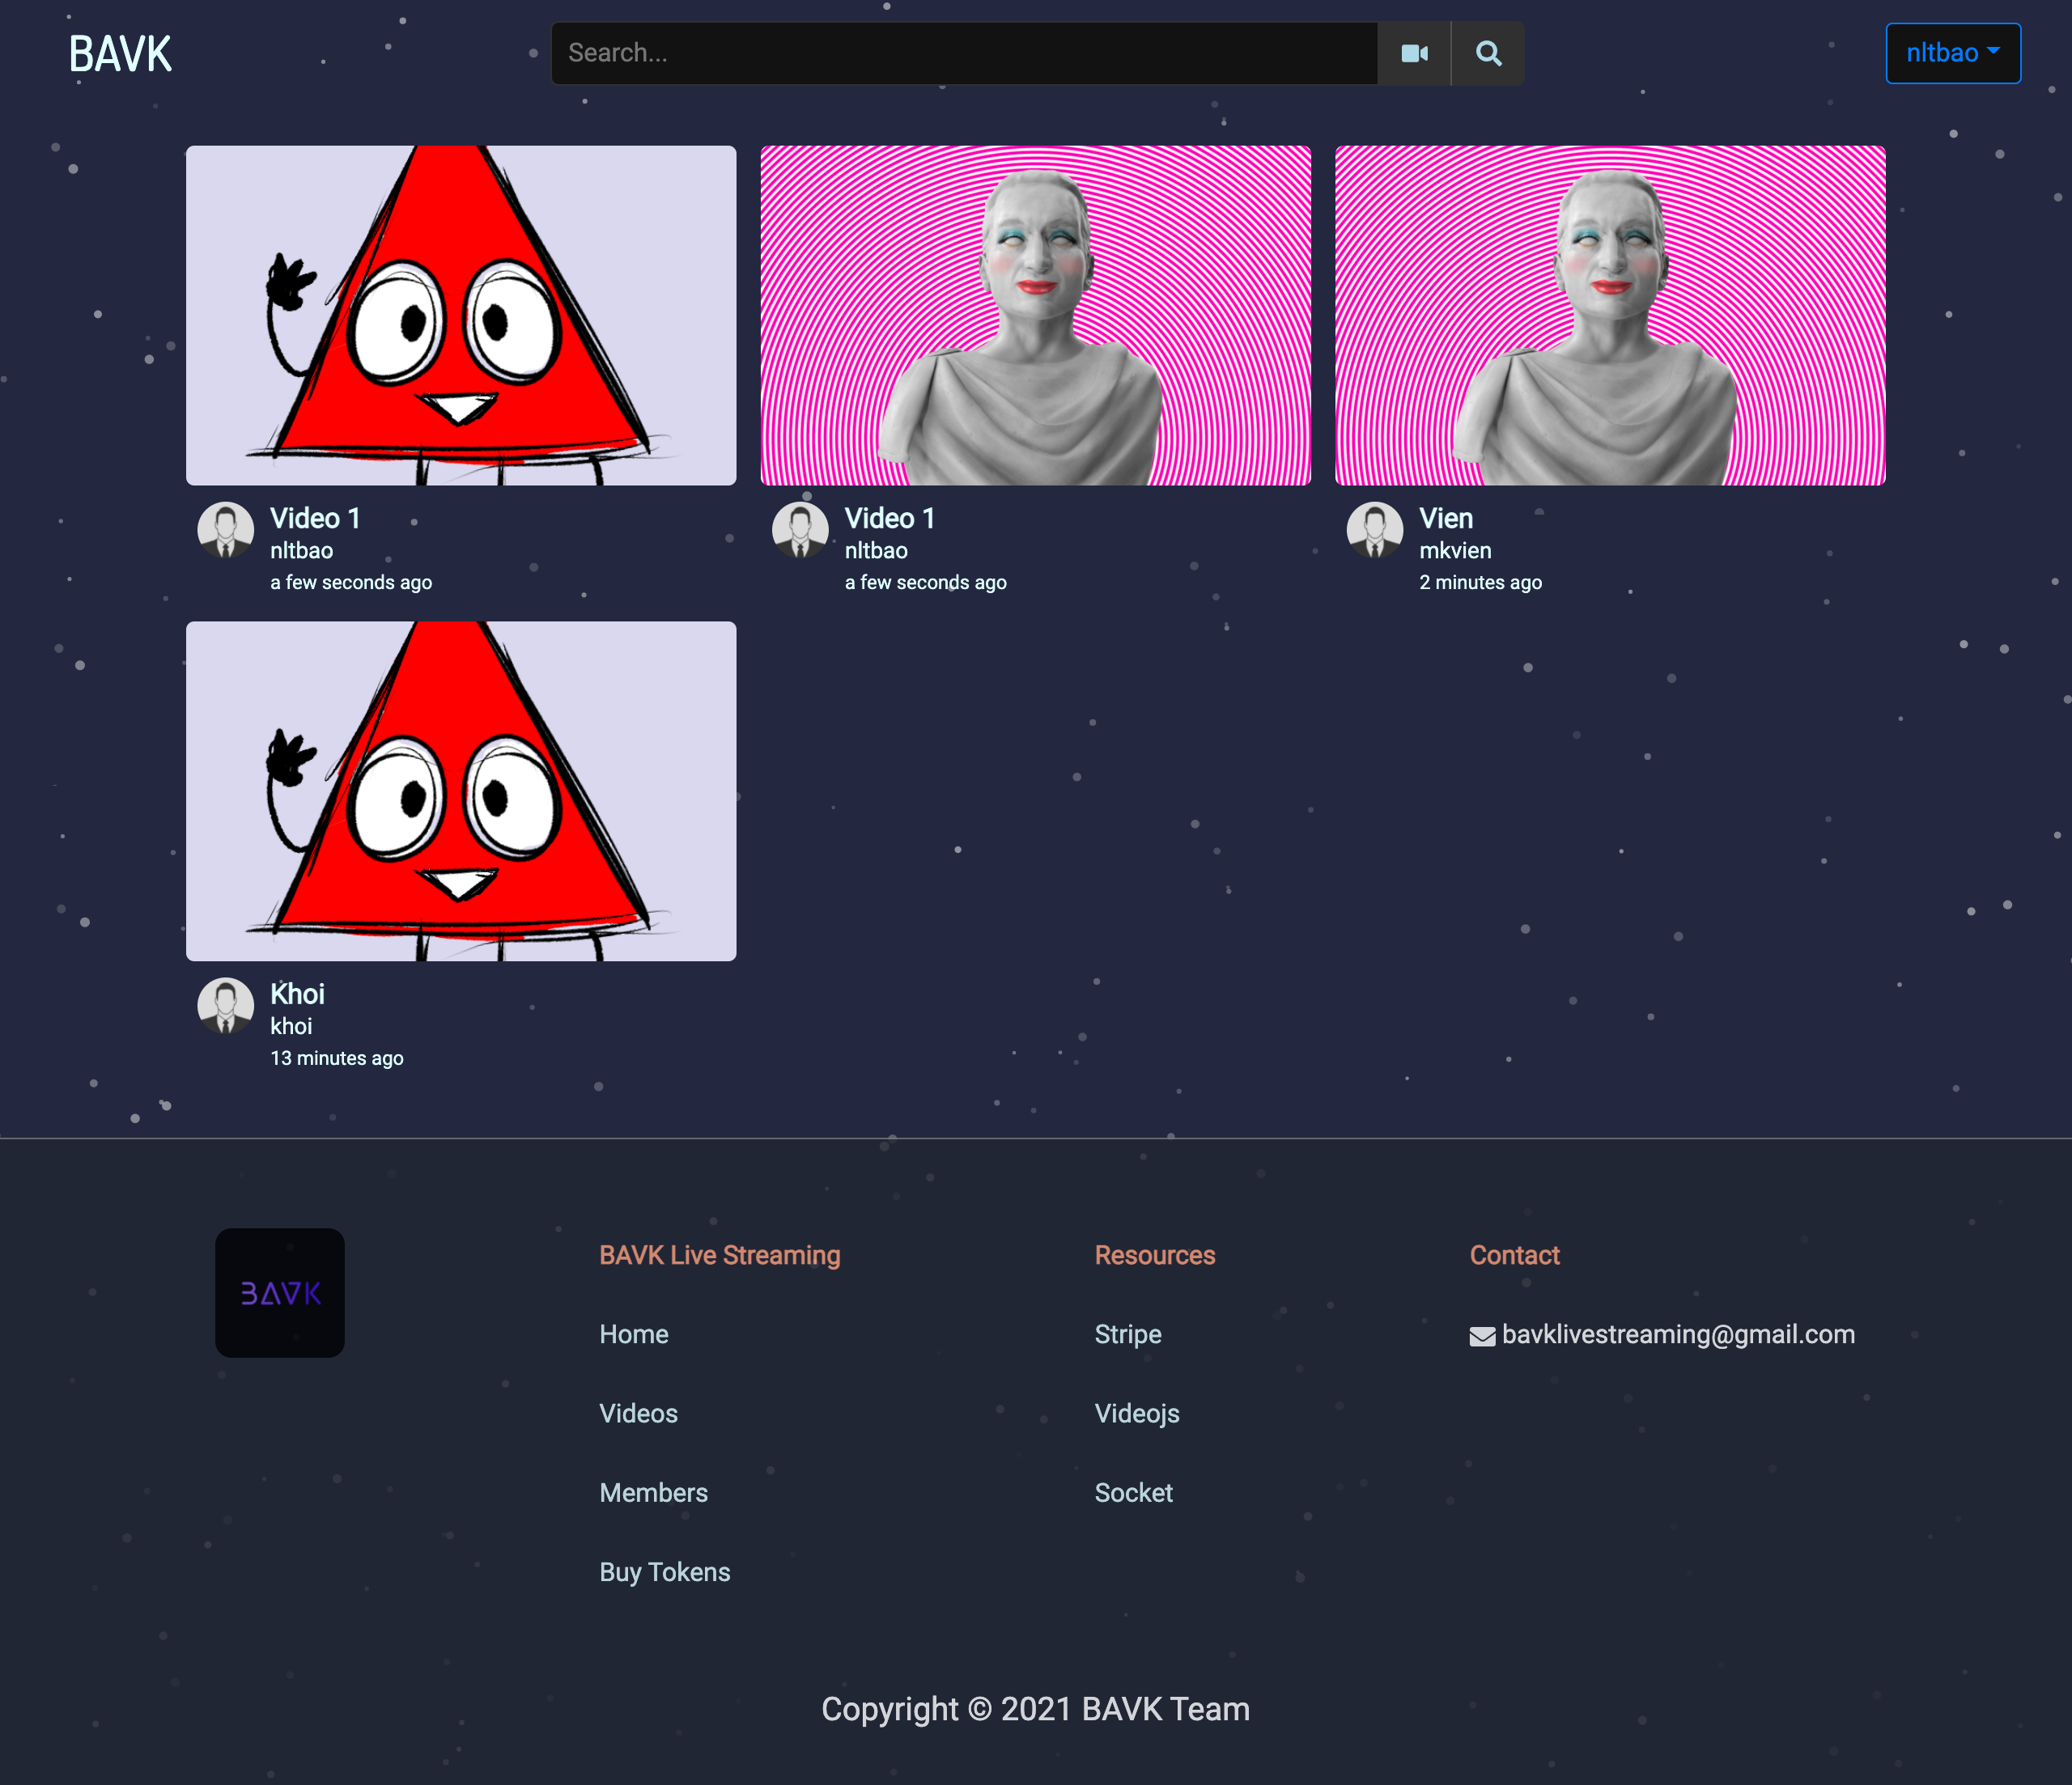
\includegraphics[width=8.5cm,height=8cm]{./imgs/layouts/videos} \\
Trang lịch sử token & Trang danh sách video \\[6pt]
\end{tabular}
\end{figure}
\end{center}

\begin{center}
\begin{figure}[H]
\begin{tabular}{cc}
  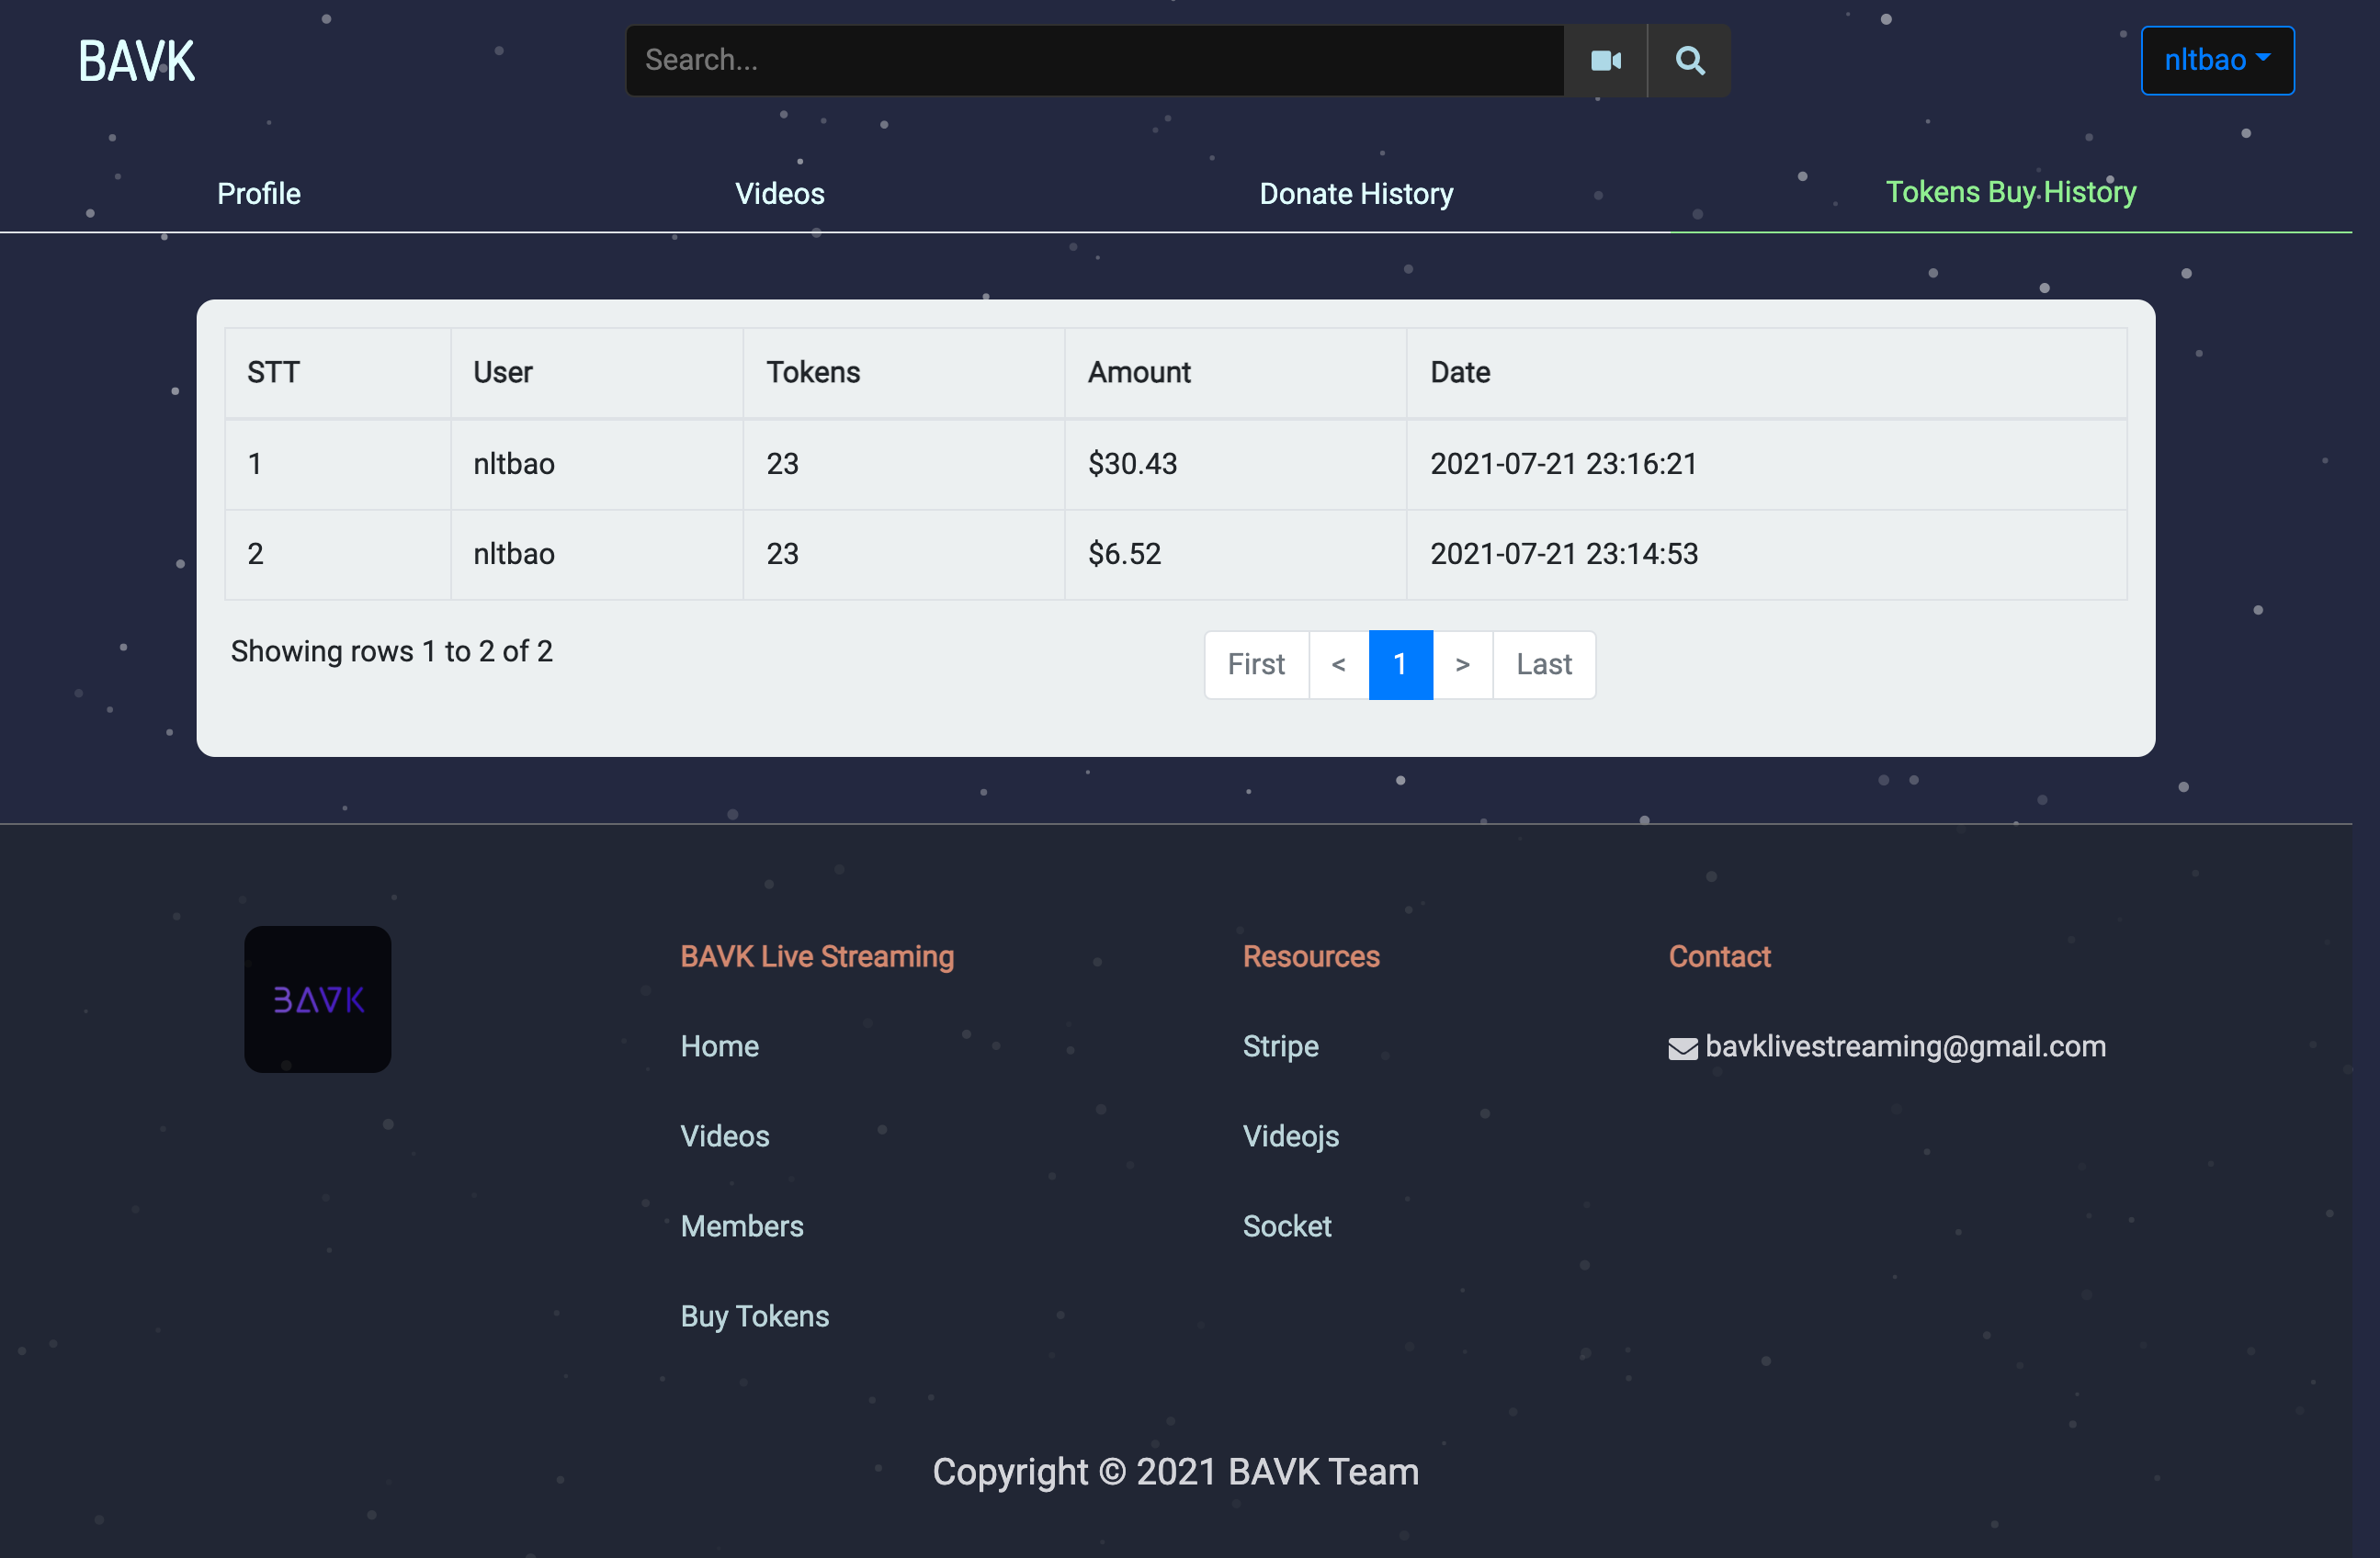
\includegraphics[width=8.5cm,height=8cm]{./imgs/layouts/history_tokens} &   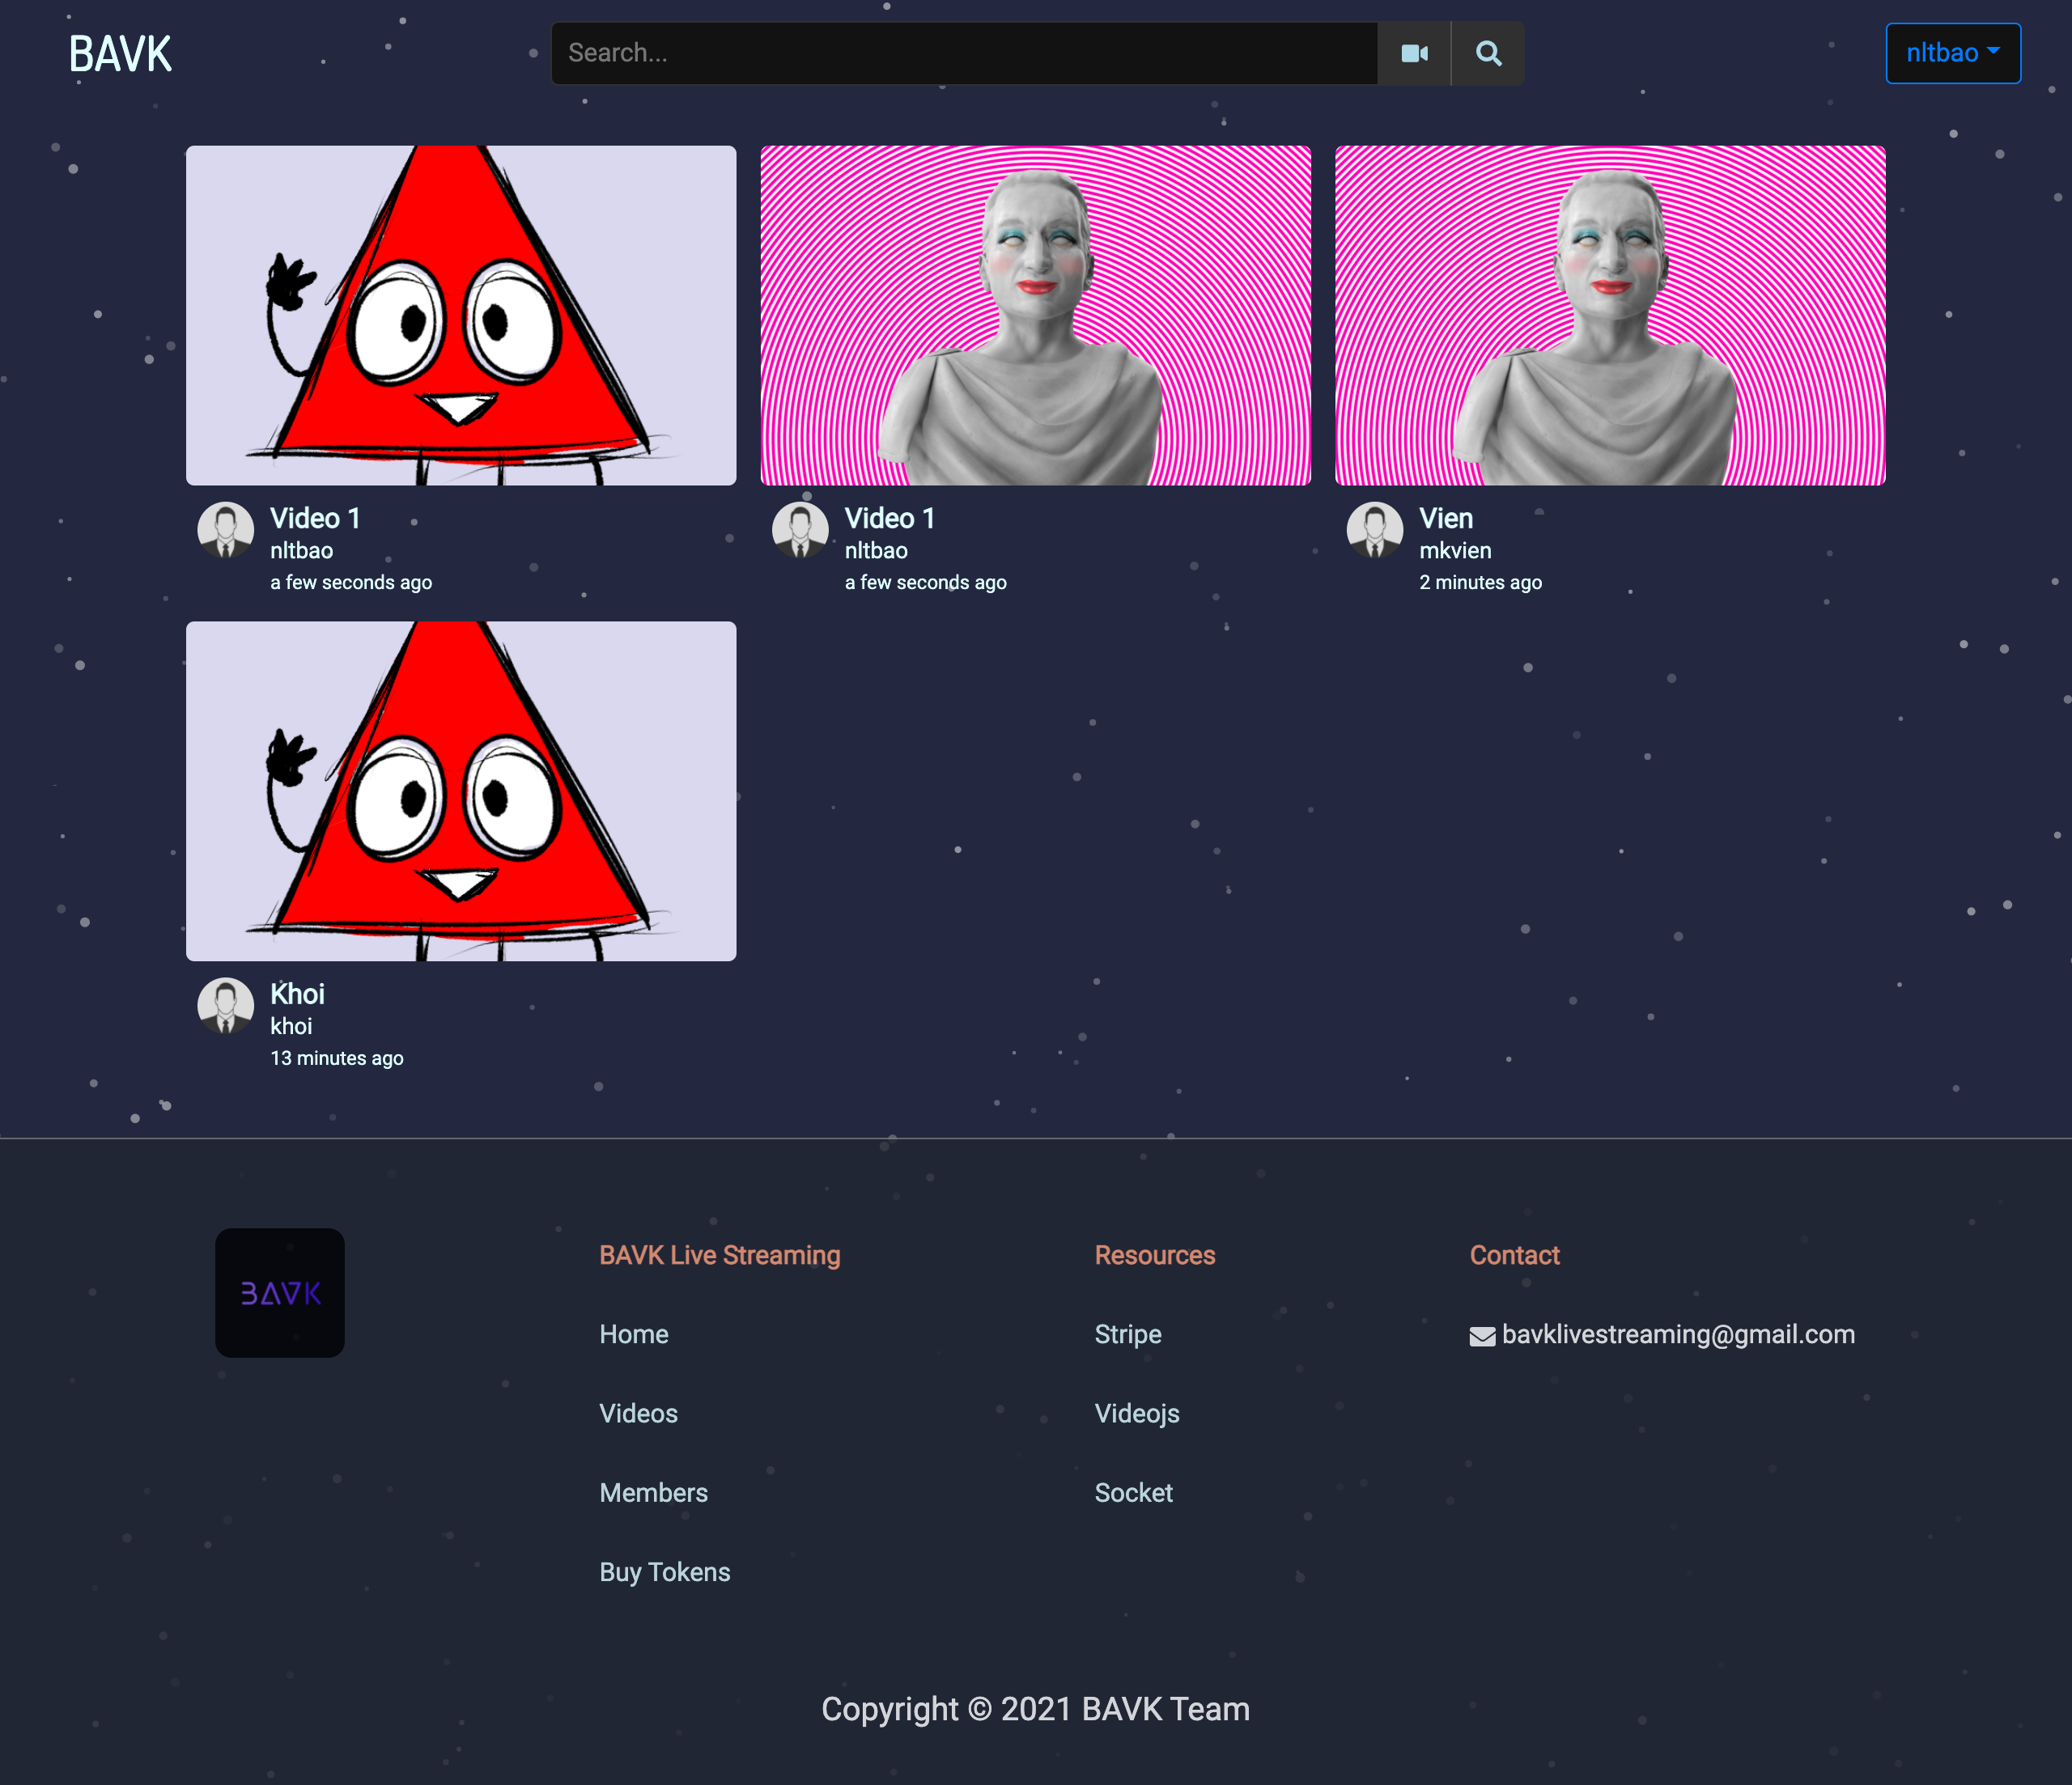
\includegraphics[width=8.5cm,height=8cm]{./imgs/layouts/videos} \\
Trang lịch sử token & Trang danh sách video \\[6pt]
\end{tabular}
\end{figure}
\end{center}

\begin{center}
\begin{figure}[H]
\begin{tabular}{cc}
  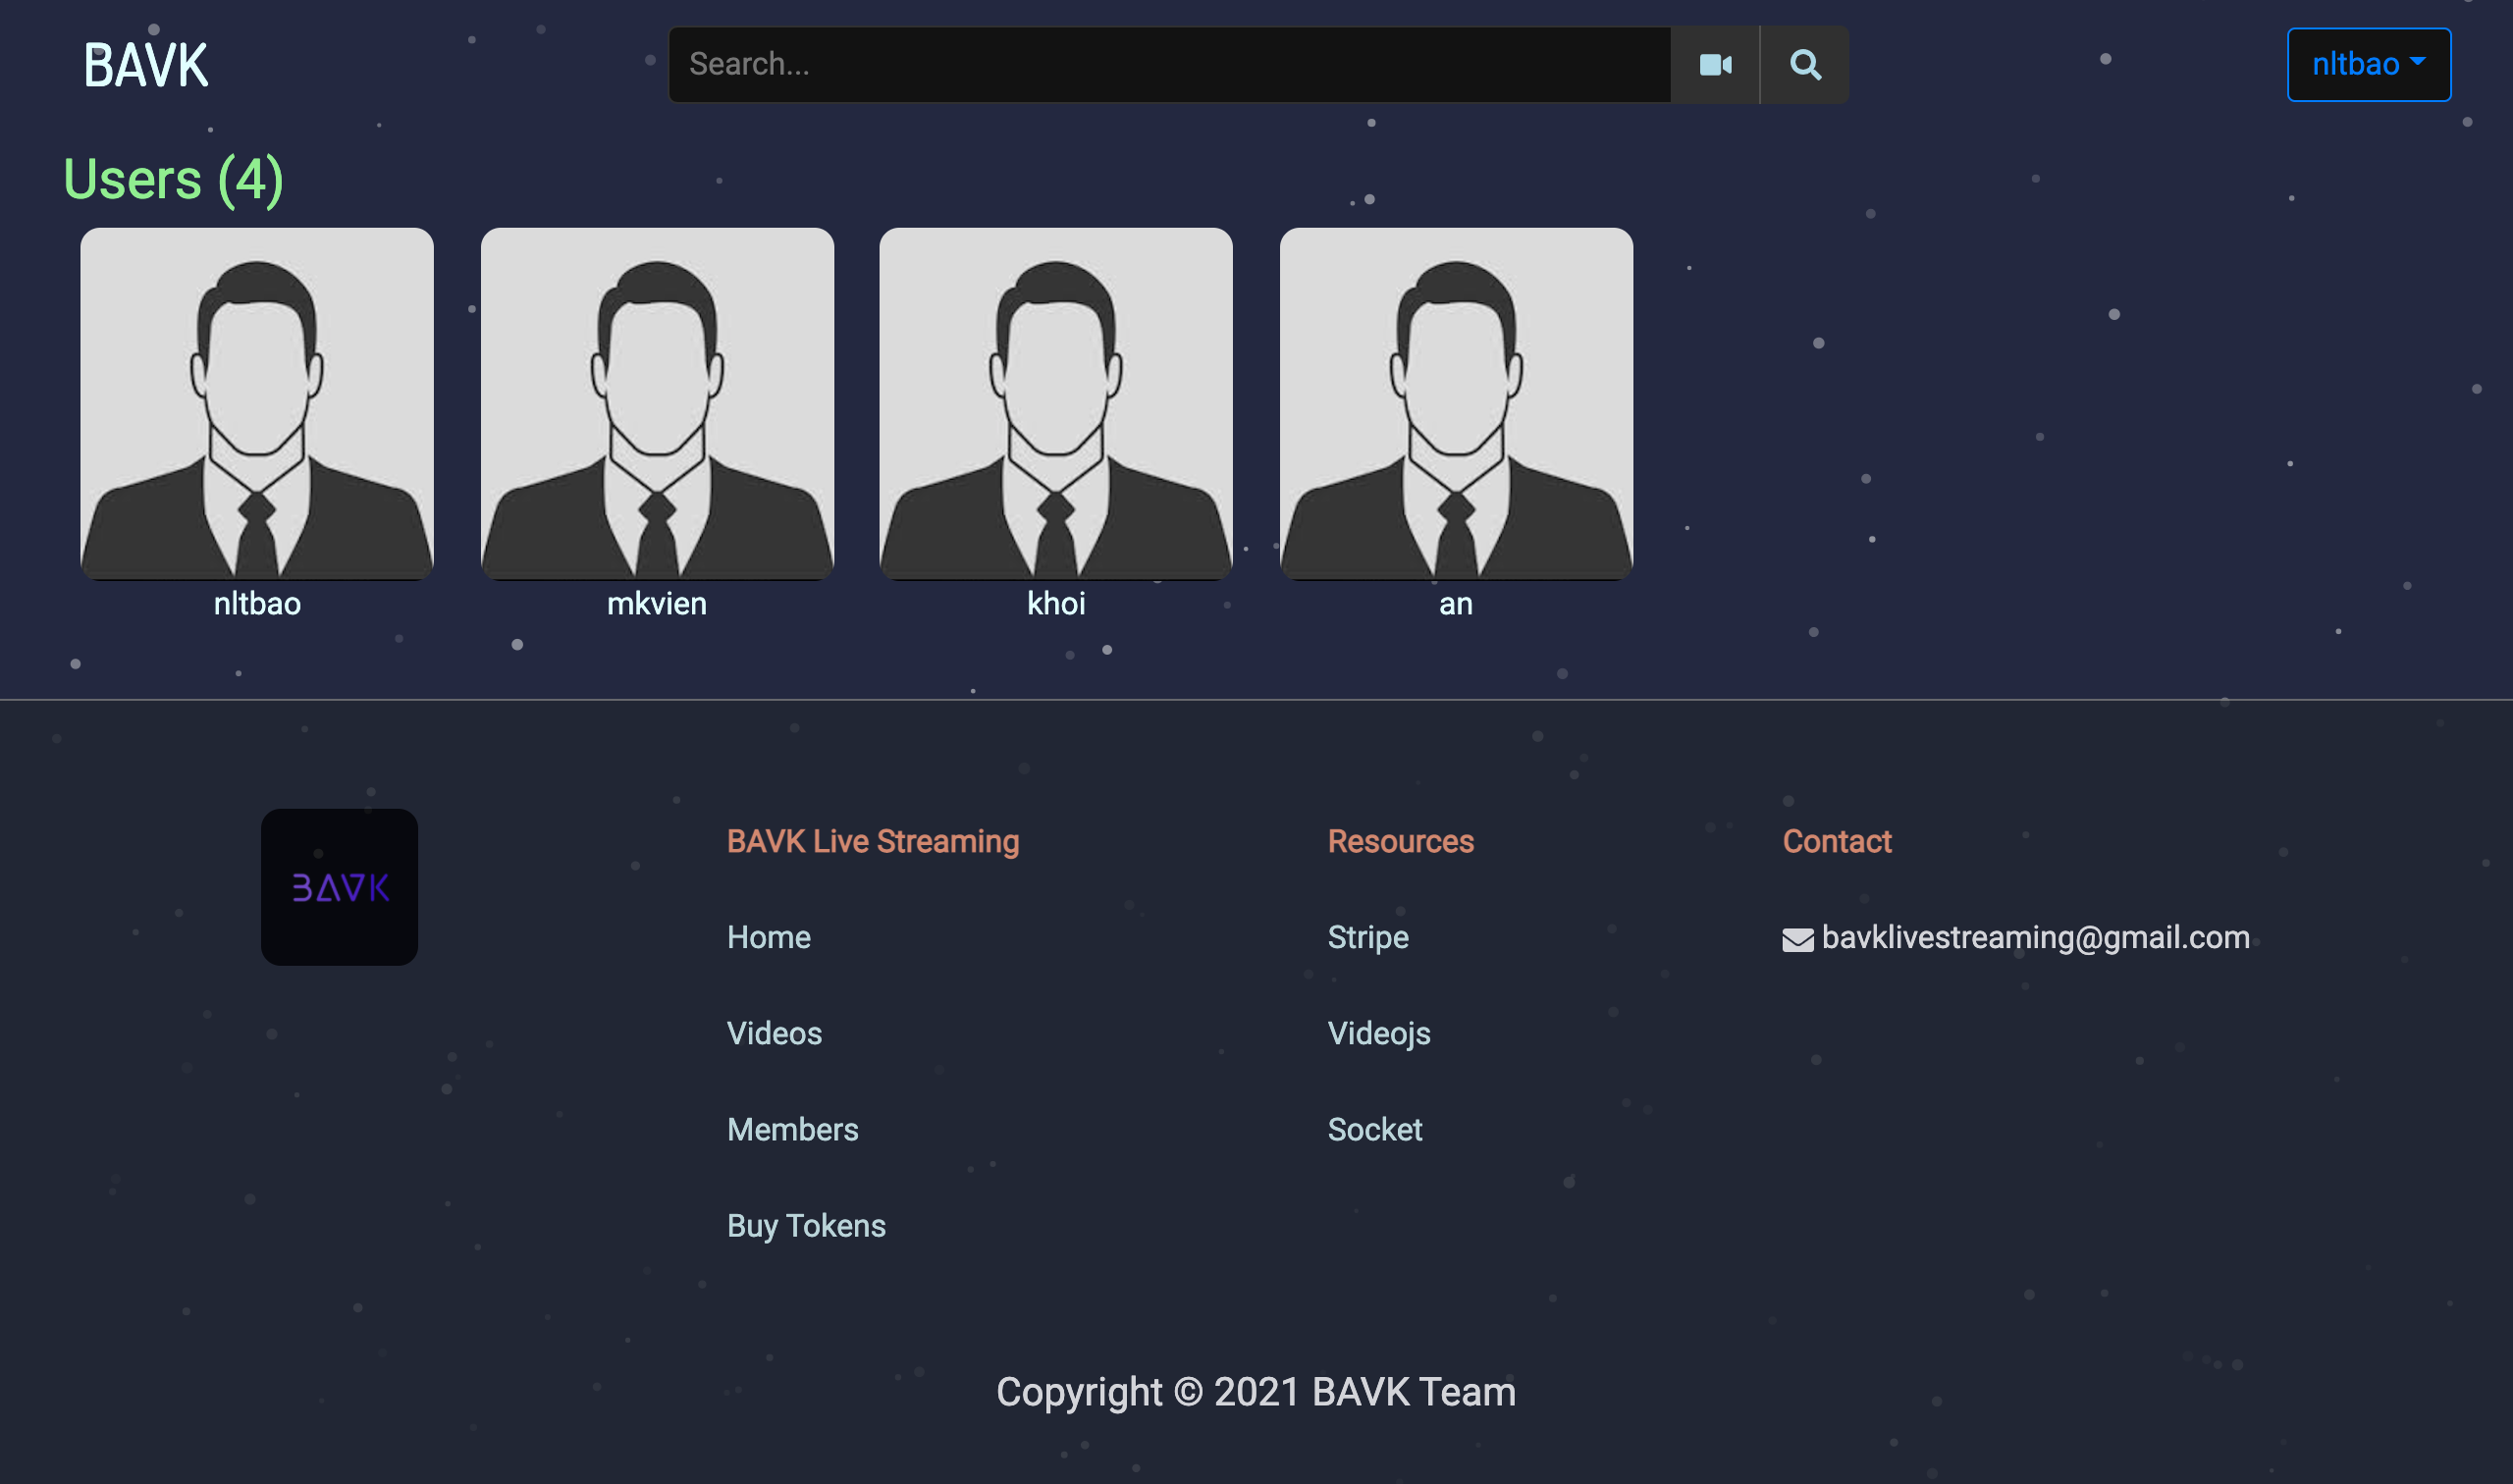
\includegraphics[width=8.5cm,height=8cm]{./imgs/layouts/users} &   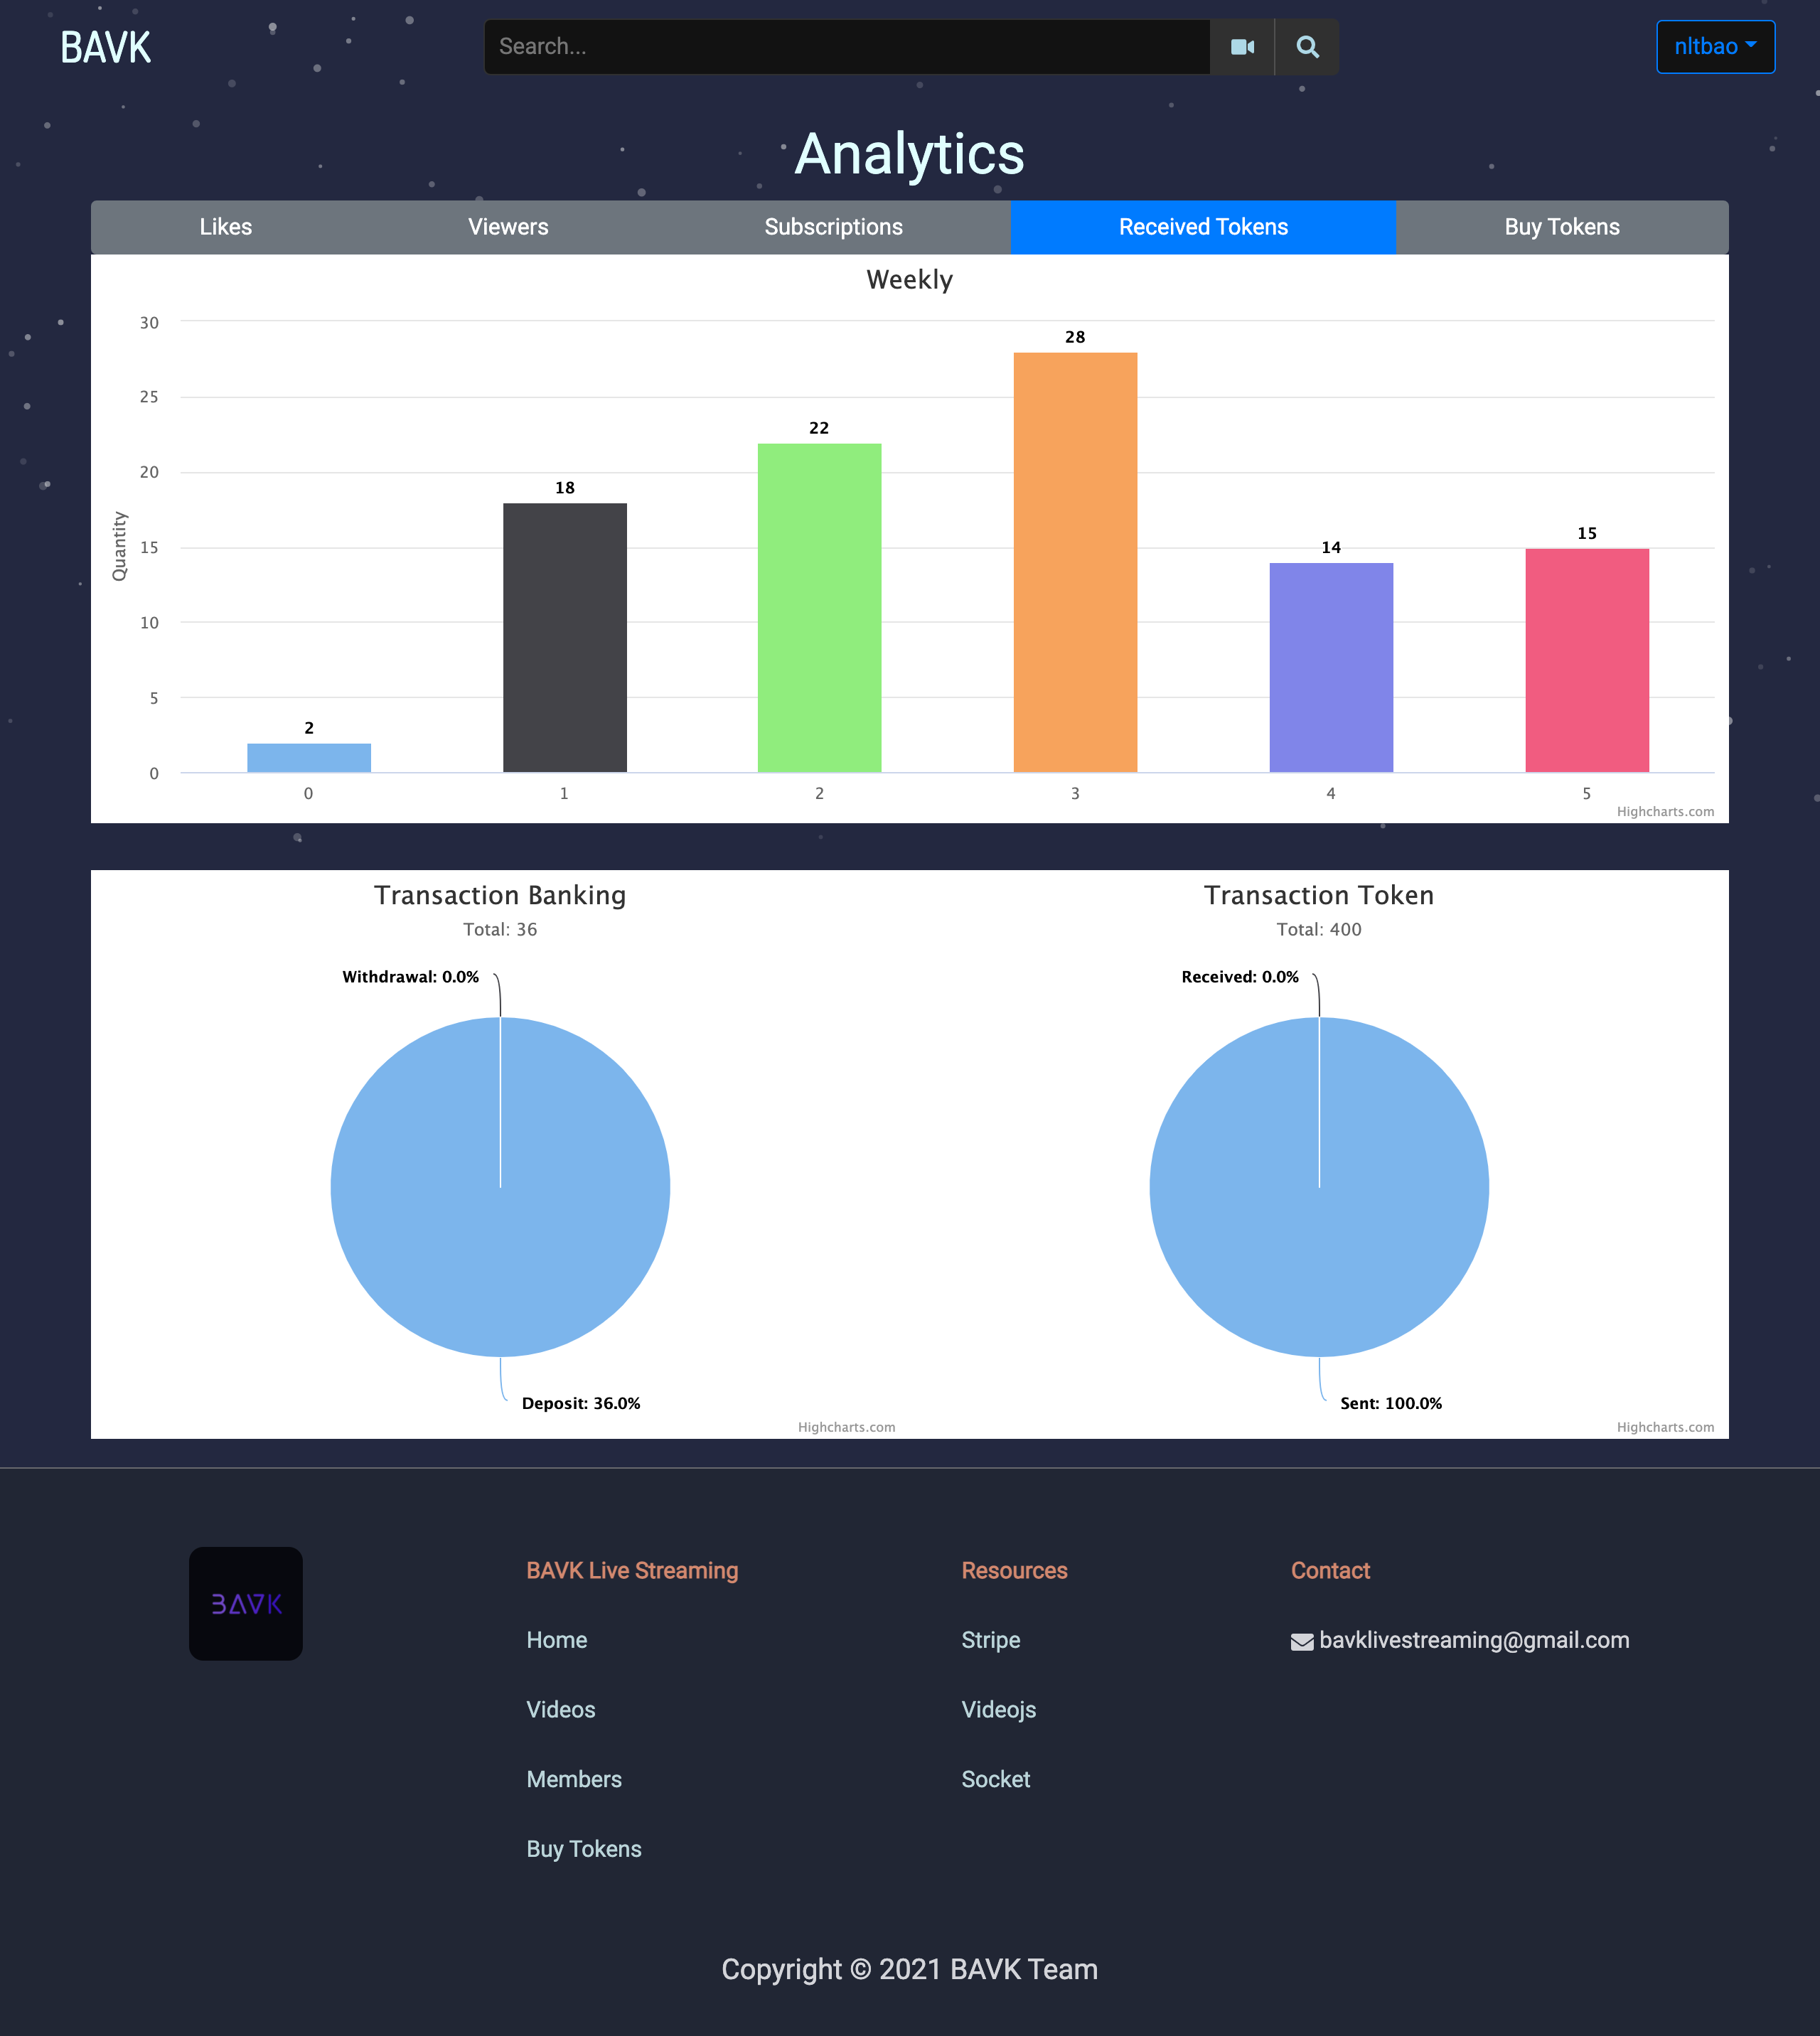
\includegraphics[width=8.5cm,height=8cm]{./imgs/layouts/statistics} \\
Trang danh sách người dùng & Trang thống kê \\[6pt]
\end{tabular}
\end{figure}
\end{center}



%%%%%%%%%%%%%%%%%%%%%%%%%%%%%%%%%%%%%%%%%%%%%%%%%%%
\section{Sơ Đồ Kiến Trúc Công Nghệ}

\section{Các Loại Sơ Đồ}
%%%%%%%%%%%%%%%%%% CONTROLLER %%%%%%%%%%%%%%%%%%
\subsection{Controller}


%%%%%%%%%%%%%%%%%% USER CONTROLLER %%%%%%%%%%%%%%%%%%

\subsubsection{User\_Controller}
\begin{center}
	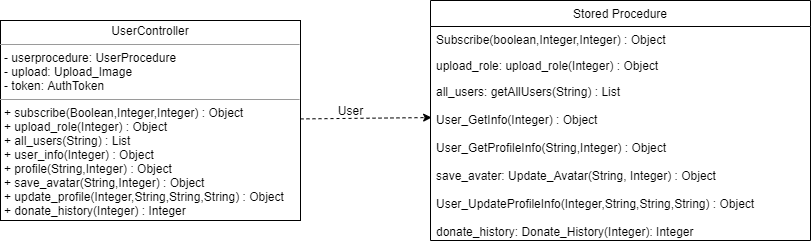
\includegraphics[width=17cm]{{./imgs/stores/user_controller}}
\end{center}

\begin{center}
\begin{longtabu} to \textwidth {| m{5cm} | m{5cm} | m{5cm} |}
\caption{Các trường} \\
   \hline \textbf{Tên}  & \textbf{Kiểu} & \textbf{Mô tả}  \\ \hline
   \endfirsthead
   \hline \textbf{Tên}  & \textbf{Kiểu} & \textbf{Mô tả}  \\ \hline
   \endhead
      userprocedure & UserProcedure  & Làm việc với dữ liệu user
      \\ \hline
      upoad & UploadImage  & Làm việc với hình ảnh
      \\ \hline
      token & AuthToken  & Làm việc với security
      \\ \hline
\end{longtabu}
\end{center}

\begin{center}
\begin{longtabu} to \textwidth {| m{3cm} | m{4cm} | m{4cm} | m{4cm} |}
\caption{Các phương thức} \\
   \hline \textbf{Tên}  & \textbf{Tham số} & \textbf{Kiểu trả về}  & \textbf{Mô tả}  \\ \hline
   \endfirsthead
   \hline \textbf{Tên}  & \textbf{Tham số} & \textbf{Kiểu trả về}  & \textbf{Mô tả}  \\ \hline
   \endhead
      subscribe & isSubcribe, hostId, followerId  & View User Layout & Truy vấn loại User hiển thị lên layout
      \\ \hline
      uploadRole & userId  & View User Layout & Chuyển đổi vai trò của tài khoản
      \\ \hline
      allUers & search  & View User danh sách & Tìm kiếm user theo từ khóa
      \\ \hline
      userInfo & userId  & View User chi tiết & Xem chi tiết user bằng mã user
      \\ \hline
      profile & nickname, hostId  & View User chi tiêt & Xem chi tiết profile 
      \\ \hline
      saveAvatar & fileName, image, userId  & View User layout & Lưu hình ảnh User
      \\ \hline
      updateProfile & id, fullName, nickName, bio  & View User Chi tiêt & Cập nhật thông tin
      \\ \hline
      donateHistory & userId  & View User Chi tiêt & Lưu thông tin donate
      \\ \hline
\end{longtabu}
\end{center}

%%%%%%%%%%%%%%%%%% STREAMER CONTROLLER %%%%%%%%%%%%%%%%%% 

\subsubsection{Streamer\_Controller}
\begin{center}
	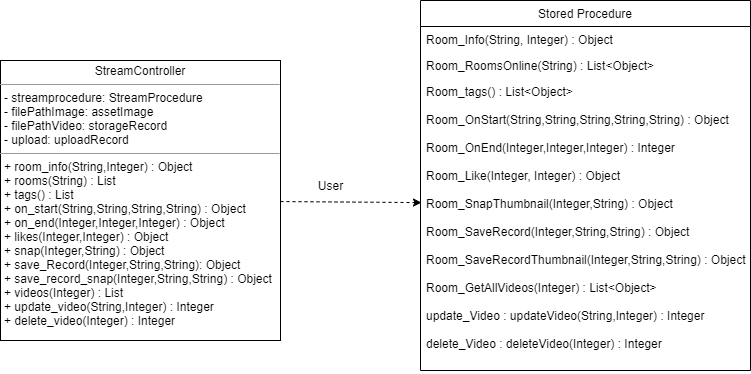
\includegraphics[width=17cm]{{./imgs/stores/streamer_controller}}
\end{center}

\begin{center}
\begin{longtabu} to \textwidth {| m{5cm} | m{5cm} | m{5cm} |}
\caption{Các trường} \\
   \hline \textbf{Tên}  & \textbf{Kiểu} & \textbf{Mô tả}  \\ \hline
   \endfirsthead
   \hline \textbf{Tên}  & \textbf{Kiểu} & \textbf{Mô tả}  \\ \hline
   \endhead
      streamprocedure & Procedure  & Làm việc với dữ liệu stream
      \\ \hline
      filePathImage & assetImage  & Làm việc với dữ liệu loại hình ảnh
      \\ \hline
      filePathVideo & storageRecord  & Làm việc với dữ liệu video
      \\ \hline
      upload & uploadRecord  & Làm việc với dữ liệu stream
      \\ \hline
\end{longtabu}
\end{center}

\begin{center}
\begin{longtabu} to \textwidth {| m{3cm} | m{4cm} | m{4cm} | m{4cm} |}
\caption{Các phương thức} \\
   \hline \textbf{Tên}  & \textbf{Tham số} & \textbf{Kiểu trả về}  & \textbf{Mô tả}  \\ \hline
   \endfirsthead
   \hline \textbf{Tên}  & \textbf{Tham số} & \textbf{Kiểu trả về}  & \textbf{Mô tả}  \\ \hline
   \endhead
      RoomInfo & roomName, idUser & View Room cụ thể & Truy vấn room hiển thị lên layout
      \\ \hline
      Rooms & search  & View List Room & Hiển thị danh sách room
      \\ \hline
      Tags &   & View List tag  & Hiển thị danh sách tag
      \\ \hline
      OnStart & userId, title, description, tag, thumbnail & View liveStream  & Bắt đầu khởi tạo video
      \\ \hline
      OnEnd & roomId, streamerId, status  & View liveStream  & Kết thúc video
      \\ \hline
      Like & StreamerId, likes  & View room  & Hiển thị số lượt thích
      \\ \hline
      Snap & fileName, UserId, image  & View liveStream  & Thêm hình ảnh
      \\ \hline
      Snap & fileName, UserId, image  & View liveStream  & Thêm hình ảnh
      \\ \hline
      SaveRecord & UserId, title, pathRecordVideo  & View liveStream lưu video  & Thực hiện lưu video
      \\ \hline
      SaveRecord & UserId, title, pathRecordVideo  & View liveStream lưu video  & Thực hiện lưu video
      \\ \hline
      SaveRecordSnap & UserId, title, patImage  & View liveStream lưu background video  & Thực hiện lưu ảnh nền cho video
      \\ \hline
      Videos & UserId  & View List video  & Hiện thị danh sách video
      \\ \hline
      VideoAll &   & UserId, title, patImage  & Danh sách video
      \\ \hline
      UpdateVideo &   & UserId, title, patImage  & Danh sách video
      \\ \hline
      DeleteVideo & VideoId  & View List video  & Xóa video
      \\ \hline
\end{longtabu}
\end{center}

%%%%%%%%%%%%%%%%%% CREDENTIAL CONTROLLER %%%%%%%%%%%%%%%%%%

\subsubsection{Credential\_Controller}
\begin{center}
	\includegraphics[width=17cm]{{./imgs/stores/credential_controller}}
\end{center}

\begin{center}
\begin{longtabu} to \textwidth {| m{5cm} | m{5cm} | m{5cm} |}
\caption{Các trường} \\
   \hline \textbf{Tên}  & \textbf{Kiểu} & \textbf{Mô tả}  \\ \hline
   \endfirsthead
   \hline \textbf{Tên}  & \textbf{Kiểu} & \textbf{Mô tả}  \\ \hline
   \endhead
      credentialprocedure & CredentialProcedure  & Làm việc với dữ liệu credential
      \\ \hline
      jwt & jsonwebtoken  & Cung cấp vấn đề bảo mật
      \\ \hline
      bcrypt & bcrypt  & Cung cấp mã hóa mật khẩu
      \\ \hline
      autToken & resetVerifyToken  & Cung cấp mã token
      \\ \hline
\end{longtabu}
\end{center}

\begin{center}
\begin{longtabu} to \textwidth {| m{3cm} | m{4cm} | m{4cm} | m{4cm} |}
\caption{Các phương thức} \\
   \hline \textbf{Tên}  & \textbf{Tham số} & \textbf{Kiểu trả về}  & \textbf{Mô tả}  \\ \hline
   \endfirsthead
   \hline \textbf{Tên}  & \textbf{Tham số} & \textbf{Kiểu trả về}  & \textbf{Mô tả}  \\ \hline
   \endhead
      Login & username, password   & View Form Login trang web & Truy vấn đăng nhập trang web
      \\ \hline
      register & username, password, nickname, email  & View Form đăng ký & Đăng ký tài khoản
      \\ \hline
      UpdatePassword & password  & View form cập nhật & Phương thức này dùng để cập nhập Lại password của tài khoản
      \\ \hline
\end{longtabu}
\end{center}

%%%%%%%%%%%%%%%%%% PAYMENT CONTROLLER %%%%%%%%%%%%%%%%%%

\subsubsection{Payment\_Controller}
\begin{center}
	\includegraphics[width=17cm]{{./imgs/stores/payment_controller}}
\end{center}

\begin{center}
\begin{longtabu} to \textwidth {| m{5cm} | m{5cm} | m{5cm} |}
\caption{Các trường} \\
   \hline \textbf{Tên}  & \textbf{Kiểu} & \textbf{Mô tả}  \\ \hline
   \endfirsthead
   \hline \textbf{Tên}  & \textbf{Kiểu} & \textbf{Mô tả}  \\ \hline
   \endhead
      paymentprocedure & PaymentProcedure  & Làm việc với kiểu dữ liệu payment
      \\ \hline
      jwt & Jsonwebtoken  & Cung cấp vấn đề bảo mật
      \\ \hline
      nodemailer & NodeMailer  & Làm việc với email
      \\ \hline
\end{longtabu}
\end{center}

\begin{center}
\begin{longtabu} to \textwidth {| m{3cm} | m{4cm} | m{4cm} | m{4cm} |}
\caption{Các phương thức} \\
   \hline \textbf{Tên}  & \textbf{Tham số} & \textbf{Kiểu trả về}  & \textbf{Mô tả}  \\ \hline
   \endfirsthead
   \hline \textbf{Tên}  & \textbf{Tham số} & \textbf{Kiểu trả về}  & \textbf{Mô tả}  \\ \hline
   \endhead
      OptionsPurchase &  & View Option payment hiện thị & Hiện thị danh sách cách thanh toán
      \\ \hline
      PurchaseToken & id, amount, idUser, nickname, currency, token & View Payment chi tiết & Lịch sử thanh toán
      \\ \hline
      DonateToken & quantity, receiver  & View Payment chi tiết & Chuyển tiền cho người nhận
      \\ \hline
      GetJwtReset & email, hostOrigin & View email & Xác nhận thanh toán qua email
      \\ \hline
      emailSender & &  View email & Gửi mã qua email
      \\ \hline
\end{longtabu}
\end{center}

%%%%%%%%%%%%%%%%%% VIDEO CONTROLLER %%%%%%%%%%%%%%%%%%

\subsubsection{Payment\_Controller}
\begin{center}
	\includegraphics[width=17cm]{{./imgs/stores/assets_video_controller}}
\end{center}

\begin{center}
\begin{longtabu} to \textwidth {| m{5cm} | m{5cm} | m{5cm} |}
\caption{Các trường} \\
   \hline \textbf{Tên}  & \textbf{Kiểu} & \textbf{Mô tả}  \\ \hline
   \endfirsthead
   \hline \textbf{Tên}  & \textbf{Kiểu} & \textbf{Mô tả}  \\ \hline
   \endhead
      assetvideopathprocedure & VideoProcedure  & Làm việc với dữ liệu video
      \\ \hline
      path & Path  & Lấy đường dẫn 
      \\ \hline
      video & string  & Làm việc với kiễu dữ liệu video
      \\ \hline
\end{longtabu}
\end{center}

\begin{center}
\begin{longtabu} to \textwidth {| m{3cm} | m{4cm} | m{4cm} | m{4cm} |}
\caption{Các phương thức} \\
   \hline \textbf{Tên}  & \textbf{Tham số} & \textbf{Kiểu trả về}  & \textbf{Mô tả}  \\ \hline
   \endfirsthead
   \hline \textbf{Tên}  & \textbf{Tham số} & \textbf{Kiểu trả về}  & \textbf{Mô tả}  \\ \hline
   \endhead
      getVideoPath & idVideo, idUser & String & Truy vấn đường dẫn video
      \\ \hline
\end{longtabu}
\end{center}

%%%%%%%%%%%%%%%%%% IMAGE CONTROLLER %%%%%%%%%%%%%%%%%%

\subsubsection{Payment\_Controller}
\begin{center}
	\includegraphics[width=17cm]{{./imgs/stores/assets_image_controller}}
\end{center}

\begin{center}
\begin{longtabu} to \textwidth {| m{5cm} | m{5cm} | m{5cm} |}
\caption{Các trường} \\
   \hline \textbf{Tên}  & \textbf{Kiểu} & \textbf{Mô tả}  \\ \hline
   \endfirsthead
   \hline \textbf{Tên}  & \textbf{Kiểu} & \textbf{Mô tả}  \\ \hline
   \endhead
      imagepathprocedure & ImageProcedure  & Làm việc với dữ liệu Image
      \\ \hline
\end{longtabu}
\end{center}

\begin{center}
\begin{longtabu} to \textwidth {| m{3cm} | m{4cm} | m{4cm} | m{4cm} |}
\caption{Các phương thức} \\
   \hline \textbf{Tên}  & \textbf{Tham số} & \textbf{Kiểu trả về}  & \textbf{Mô tả}  \\ \hline
   \endfirsthead
   \hline \textbf{Tên}  & \textbf{Tham số} & \textbf{Kiểu trả về}  & \textbf{Mô tả}  \\ \hline
   \endhead
      getImagePath & filePath & String & Hiển thị hình ảnh
      \\ \hline
\end{longtabu}
\end{center}



%%%%%%%%%%%%%%%%%% SERVICE %%%%%%%%%%%%%%%%%%
\subsection{Service}

%%%%%%%%%%%%%%%%%% EMAIL SERVICE %%%%%%%%%%%%%%%%%%
\subsubsection{Email Service}

\begin{center}
	\includegraphics[width=17cm]{{./imgs/diagrams/email_service}}
\end{center}

\begin{center}
\begin{longtabu} to \textwidth {| m{3cm} | m{4cm} | m{4cm} | m{4cm} |}
\caption{Mô tả} \\
   \hline \textbf{Tên}  & \textbf{Tham số} & \textbf{Kiểu trả về}  & \textbf{Mô tả}  \\ \hline
   \endfirsthead
   \hline \textbf{Tên}  & \textbf{Tham số} & \textbf{Kiểu trả về}  & \textbf{Mô tả}  \\ \hline
   \endhead
      getImagePath & filePath & String & Hiển thị hình ảnh
      \\ \hline
\end{longtabu}
\end{center}






\chapter{KIỂM THỬ}

\begin{center}
\begin{landscape}
\footnotesize
\begin{longtabu} to \textwidth {| p{1cm} | p{2.5cm} | p{2.5cm} | p{4.5cm} | p{4.5cm} | p{4.5cm} | p{2cm} | p{1.5cm} |}
\caption{Bảng kiểm thử} \\
   \hline \textbf{STT}  & \textbf{Test Case} & \textbf{Actions} & \textbf{Input data} & \textbf{Expected Results} & \textbf{Test Results} & \textbf{Date Verified} & \textbf{Status} \\ \hline
   \endfirsthead
  \hline \textbf{STT}  & \textbf{Test Case} & \textbf{Actions} & \textbf{Input data} & \textbf{Expected Results} & \textbf{Test Results} & \textbf{Date Verified} & \textbf{Status} \\ \hline
   \endhead
      %%%%%%%%%%%%% 1 %%%%%%%%%%%%%
      \begin{itemize}[leftmargin=*,label={}]
      \item 1
      \end{itemize} 
      & 
      \begin{itemize}[leftmargin=*,label={}]
      \item Form đăng ký  
      \end{itemize}
      & 
      \begin{itemize}[leftmargin=*,label={}]
      \item Tạo tài khoản 
      \end{itemize}
      & 
      \begin{itemize}[leftmargin=*]
      \item[1/] Nhấn vào button login
      \item[2/] Nhấn vào đường dẫn Create Account
      \item[3/] Nhập thông tin dữ liệu: "Nickname", "Email", "Username", "Password"
      \item[4/] Nhấn Register
      \end{itemize}
       & 
      \begin{itemize}[leftmargin=*]
      \item[1/] "an1234", "anntps12@gmail.com", "anntps10672", "anntps10671"
      \item[2/] "null", "anntps12@gmail.com", "anntps10672", "anntps10671"
      \item[3/] "\@\@\#\$", "anntps12@gmail.com", "anntps10672", "anntps10671"
      \item[4/] "an1234", "\!\@\#2323\_\@gmail.com", "anntps10672", "anntps10671"
      \item[4/] "an1234", "123@gmail.com", "anntps10672", "anntp10671"
      \end{itemize}
       & 
      \begin{itemize}[leftmargin=*]
      \item[1/] Hiển thị thông báo: "Register successfully"
      \item[2/] Hiển thị thông báo: "Nick name không được để trống"
      \item[3/] Hiển thị thông báo: "Email  chỉ được phép sử dụng các chữ cái (a-z),số (0-9), và dấu chấm"
      \item[4/] Hiển thị thông báo: "Mật khẩu độ dài 8-16 ký tự, có ít nhất 1 chữ cái (a-z hoặc A-Z) và 1 chữ số, và không giống với tên tài khoản."
      \end{itemize}
        &
      \begin{itemize}[leftmargin=*,label={}]
      \item 08/07/2021 
      \end{itemize} 
        & 
      \begin{itemize}[leftmargin=*,label={}]
      \item Passed 
      \end{itemize} 
      \\ \hline
      %%%%%%%%%%%%% 2 %%%%%%%%%%%%%
      \begin{itemize}[leftmargin=*,label={}]
      \item 2 
      \end{itemize} 
      &
      \begin{itemize}[leftmargin=*,label={}]
      \item Form đăng nhập  
      \end{itemize}
      & 
      \begin{itemize}[leftmargin=*,label={}]
      \item Đăng nhập tài khoản 
      \end{itemize}
      & 
      \begin{itemize}[leftmargin=*]
      \item[1/] Nhấn vào button login
      \item[2/] Nhập username + password
      \item[3/] Nhấn đăng nhập
      \end{itemize}
       & 
      \begin{itemize}[leftmargin=*]
      \item[1/] "anntps10672", "anntps10671"
      \item[2/] "null", "null"
      \item[3/] "123", "anntps10671"
      \end{itemize}
       & 
      \begin{itemize}[leftmargin=*]
      \item[1/] Hiển thị thông báo: "Login successfully"
      \item[2/] Hiển thị thông báo: "Vui lòng không được để trống"
      \item[3/] Hiển thị thông báo: "User name or password incorrect"
      \end{itemize}
        &
      \begin{itemize}[leftmargin=*,label={}]
      \item 08/07/2021 
      \end{itemize} 
        & 
      \begin{itemize}[leftmargin=*,label={}]
      \item Passed
      \end{itemize}
      \\ \hline
      %%%%%%%%%%%%% 3 %%%%%%%%%%%%%
      \begin{itemize}[leftmargin=*,label={}]
      \item 3 
      \end{itemize} 
      &
      \begin{itemize}[leftmargin=*,label={}]
      \item Form đổi mật khẩu 
      \end{itemize}
      & 
      \begin{itemize}[leftmargin=*,label={}]
      \item Đổi mật khẩu tài khoản
      \end{itemize}
      & 
      \begin{itemize}[leftmargin=*]
      \item[1/] Nhấn vào button login chọn forgot password và điền email của tài khoản đã đăng ký để đổi mật khẩu
      \item[2/] Sau khi có link từ email. Điều hướng tới trang đổi mật khẩu. Điền mật khẩu mới và xác nhận mật khẩu mới
      \end{itemize}
       & 
      \begin{itemize}[leftmargin=*]
      \item[1/] "anntps10672@fpt.edu.vn"
      \item[2/] "anntps10672"
      \item[3/] "password", "123456"
      \item[4/] "password", "password"
      \end{itemize}
       & 
      \begin{itemize}[leftmargin=*]
      \item[1/] Hiển thị thông báo: "Thành công. Vui lòng check email để thay đổi mật khẩu"
      \item[2/] Hiển thị thông báo: "Định dạng email không hợp lệ"
      \item[3/] Hiển thị thông báo: "Mật khẩu xác nhận không khớp"
      \item[4/] Hiển thị thông báo: "Đổi mật khẩu thành công"
      \end{itemize}
        &
      \begin{itemize}[leftmargin=*,label={}]
      \item 10/07/2021 
      \end{itemize} 
        & 
      \begin{itemize}[leftmargin=*,label={}]
      \item Passed
      \end{itemize}
      \\ \hline
      %%%%%%%%%%%%% 4 %%%%%%%%%%%%%
      \begin{itemize}[leftmargin=*,label={}]
      \item 4 
      \end{itemize} 
      &
      \begin{itemize}[leftmargin=*,label={}]
      \item Form đăng xuất 
      \end{itemize}
      & 
      \begin{itemize}[leftmargin=*,label={}]
      \item Đăng xuất
      \end{itemize}
      & 
      \begin{itemize}[leftmargin=*]
      \item[1/] Click vào menu chính sau đó clikc vào "Logout"
      \end{itemize}
       & 
       & 
      \begin{itemize}[leftmargin=*]
      \item[1/] Hiển thị thông báo: "Đăng xuất thành công"
      \end{itemize}
        &
      \begin{itemize}[leftmargin=*,label={}]
      \item 15/07/2021 
      \end{itemize} 
        & 
      \begin{itemize}[leftmargin=*,label={}]
      \item Passed
      \end{itemize}
      \\ \hline
      %%%%%%%%%%%%% 5 %%%%%%%%%%%%%
      \begin{itemize}[leftmargin=*,label={}]
      \item 5
      \end{itemize}
      & 
      \begin{itemize}[leftmargin=*,label={}]
      \item Quản lý trang 
      \end{itemize}
      & 
      \begin{itemize}[leftmargin=*,label={}]
      \item Điều hướng trang  
      \end{itemize}
      & 
      \begin{itemize}[leftmargin=*]
      \item[1/] Nhấn vào đường biểu tượng trang chủ
      \item[2/] Từ menu chính, nhấn vào "Go Live"
      \item[3/] Từ menu chính, nhấn vào "Profile"
      \item[4/] Từ menu chính, nhấn vào "List Members"
      \item[5/] Từ menu chính, nhấn vào "List Videos"
      \item[6/] Từ menu chính, nhấn vào "Buy Tokens"
      \end{itemize}
       & 
       & 
      \begin{itemize}[leftmargin=*]
      \item[1/] Điều hướng tới "/"
      \item[2/] Điều hướng tới "/streamer"
      \item[3/] Điều hướng tới "/profile:user"
      \item[4/] Điều hướng tới "/member"
      \item[5/] Điều hướng tới "/buy\_tokens"      
      \end{itemize}
       &
      \begin{itemize}[leftmargin=*,label={}]
      \item 08/07/2021  
      \end{itemize}
        & 
      \begin{itemize}[leftmargin=*,label={}]
      \item Passed 
      \end{itemize}
      \\ \hline
      %%%%%%%%%%%%% 6 %%%%%%%%%%%%%
      \begin{itemize}[leftmargin=*,label={}]
      \item 6 
      \end{itemize} 
      & 
      \begin{itemize}[leftmargin=*,label={}]
      \item  Chuyển đổi vai trò
      \end{itemize}
      & 
      \begin{itemize}[leftmargin=*,label={}]
      \item Get quyền được "Live Stream" 
      \end{itemize}
      & 
      \begin{itemize}[leftmargin=*]
      \item[1/] Từ menu chính, click vào "Enable Live" (trừ trường hợp chưa đổi vai trò trước đó)
      \end{itemize}
       & 
       & 
      \begin{itemize}[leftmargin=*]
      \item[1/] Hiển thị thông báo "Thành công"
      \end{itemize}
        &
      \begin{itemize}[leftmargin=*,label={}]
      \item 15/07/2021 
      \end{itemize} 
        & 
      \begin{itemize}[leftmargin=*,label={}]
      \item Passed
      \end{itemize} 
      \\ \hline
      %%%%%%%%%%%%% 7 %%%%%%%%%%%%%
      \begin{itemize}[leftmargin=*,label={}]
      \item 7 
      \end{itemize} 
      & 
      \begin{itemize}[leftmargin=*,label={}]
      \item  Trang live stream
      \end{itemize}
      & 
      \begin{itemize}[leftmargin=*,label={}]
      \item Chức năng live stream
      \end{itemize}
      & 
      \begin{itemize}[leftmargin=*]
      \item[1/] Điền "Title", "Description", "Tags" cho video
      \item[2/] Click vào nút "Start" để bắt đầu live stream 
      \end{itemize}
       &
       \begin{itemize}[leftmargin=*]
      \item[1/] "title", "description", "talkshow, gaming"
      \end{itemize}
       & 
      \begin{itemize}[leftmargin=*]
      \item[1/] Hiển thị phòng ra ngoài trang chủ
      \item[2/] Gửi email tới các user đã "Subscribe" kênh
      \end{itemize}
        &
      \begin{itemize}[leftmargin=*,label={}]
      \item 20/07/2021 
      \end{itemize} 
        & 
      \begin{itemize}[leftmargin=*,label={}]
      \item Passed
      \end{itemize} 
      \\ \hline
      %%%%%%%%%%%%% 8 %%%%%%%%%%%%%
      \begin{itemize}[leftmargin=*,label={}]
      \item 8 
      \end{itemize} 
      & 
      \begin{itemize}[leftmargin=*,label={}]
      \item  Trang live stream
      \end{itemize}
      & 
      \begin{itemize}[leftmargin=*,label={}]
      \item Các chức năng trong quá trình live stream của streamer
      \end{itemize}
      & 
      \begin{itemize}[leftmargin=*]
      \item[1/] Chat với người xem
      \item[2/] Chặn chat người xem (với các trường hợp spam, thả thính)
      \item[3/] Xem danh sách người xem đã chặn
      \item[4/] Xem số lượt người đang xem
      \item[5/] Ghi hình video
      \item[6/] Kết thúc ghi hình. Thiết lập thumbnail, title cho video
      \item[7/] Kết thúc live stream
      \end{itemize}
       &
       \begin{itemize}[leftmargin=*]
      \item[1/] "Hello con dân của ta"
      \end{itemize}
       & 
      \begin{itemize}[leftmargin=*]
      \item[1/] Người xem có thể thấy được tin nhắn từ streamer
      \item[2/] Chặn chat và thông báo tới người bị chặn.
      \item[3/] 
      \item[4/] 
      \item[5/]
      \item[6/] Nhận được thông báo: "Đã lưu video"
      \item[7/] Gửi thông báo kết thúc live stream tới người xem
      \end{itemize}
        &
      \begin{itemize}[leftmargin=*,label={}]
      \item 07/08/2021 
      \end{itemize} 
        & 
      \begin{itemize}[leftmargin=*,label={}]
      \item Passed
      \end{itemize} 
      \\ \hline
     %%%%%%%%%%%%% 9 %%%%%%%%%%%%%
      \begin{itemize}[leftmargin=*,label={}]
      \item 9 
      \end{itemize} 
      & 
      \begin{itemize}[leftmargin=*,label={}]
      \item  Trang xem video đang streaming
      \end{itemize}
      & 
      \begin{itemize}[leftmargin=*,label={}]
      \item Các chức năng của viewer
      \end{itemize}
      & 
      \begin{itemize}[leftmargin=*]
      \item[1/] Chat với streamer
      \item[2/] Nhập số lượng tokens kèm lời nhắn để donate cho streamer
      \item[3/] Thích 
      \item[4/] Xem số lượt người đang xem 
      \end{itemize}
       &
       \begin{itemize}[leftmargin=*]
      \item[1/] "Hello streamer"
      \item[2/] "100 tokens", "donate"
      \item[3/] 
      \item[4/] 
      \end{itemize}
       & 
      \begin{itemize}[leftmargin=*]
      \item[1/] Streamer nhận được dòng chat từ viewer
      \item[2/] Hiển thị thông báo donate broadcast từ người xem kèm lời nhắn và số lượng token
      \item[3/] Tăng số lượt thích phòng
      \item[4/] 
      \end{itemize}
        &
      \begin{itemize}[leftmargin=*,label={}]
      \item 07/08/2021 
      \end{itemize} 
        & 
      \begin{itemize}[leftmargin=*,label={}]
      \item Passed
      \end{itemize} 
      \\ \hline
      %%%%%%%%%%%%% 10 %%%%%%%%%%%%%
      \begin{itemize}[leftmargin=*,label={}]
      \item 10 
      \end{itemize} 
      & 
      \begin{itemize}[leftmargin=*,label={}]
      \item  Donate 
      \end{itemize}
      & 
      \begin{itemize}[leftmargin=*,label={}]
      \item Chức năng donate
      \end{itemize}
      & 
      \begin{itemize}[leftmargin=*]
      \item[1/] Nhập tokens
      \item[2/] Nhập lời nhắn
      \end{itemize}
       &
       \begin{itemize}[leftmargin=*]
      \item[1/] 1000, "Donate"
      \item[2/] 500,  "Donate"
      \end{itemize}
       & 
      \begin{itemize}[leftmargin=*]
      \item[1/] Hiển thị thông báo "Bạn không đủ tokens"
      \item[2/] Hiển thị thông báo "Donate thành công". Sau đó gửi thông báo broadcast tới phòng streamer
      \end{itemize}
        &
      \begin{itemize}[leftmargin=*,label={}]
      \item 10/08/2021 
      \end{itemize} 
        & 
      \begin{itemize}[leftmargin=*,label={}]
      \item Passed
      \end{itemize} 
      \\ \hline
      %%%%%%%%%%%%% 11 %%%%%%%%%%%%%
      \begin{itemize}[leftmargin=*,label={}]
      \item 11 
      \end{itemize} 
      & 
      \begin{itemize}[leftmargin=*,label={}]
      \item  Profile 
      \end{itemize}
      & 
      \begin{itemize}[leftmargin=*,label={}]
      \item Trang quản lý thông tin
      \end{itemize}
      & 
      \begin{itemize}[leftmargin=*]
      \item[1/] Thay đổi avatar
      \item[2/] Thay đổi họ tên
      \item[3/] Thay đổi nickname
      \item[4/] Thay đổi bio
      \end{itemize}
       &
       \begin{itemize}[leftmargin=*]
      \item[1/] 
      \item[2/] "Nguyễn Trường An"
      \item[3/] "antn"
      \item[4/] "Hello"
      \end{itemize}
       & 
      \begin{itemize}[leftmargin=*]
      \item[1/] Hiển thị thông báo "Thành công"
      \item[2/] Hiển thị thông báo "Thành công"
      \item[3/] Hiển thị thông báo "Thành công"
      \item[4/] Hiển thị thông báo "Thành công"
      \end{itemize}
        &
      \begin{itemize}[leftmargin=*,label={}]
      \item 12/08/2021 
      \end{itemize} 
        & 
      \begin{itemize}[leftmargin=*,label={}]
      \item Passed
      \end{itemize} 
      \\ \hline
      %%%%%%%%%%%%% 12 %%%%%%%%%%%%%
      \begin{itemize}[leftmargin=*,label={}]
      \item 12 
      \end{itemize} 
      & 
      \begin{itemize}[leftmargin=*,label={}]
      \item  Quản lý video 
      \end{itemize}
      & 
      \begin{itemize}[leftmargin=*,label={}]
      \item Trang quản lý video
      \end{itemize}
      & 
      \begin{itemize}[leftmargin=*]
      \item[1/] Xem video ghi hình đã lưu
      \item[2/] Chỉnh sửa thông tin video
      \item[3/] Xoá video đã lưu
      \end{itemize}
       &
       \begin{itemize}[leftmargin=*]
      \item[1/] 
      \item[2/] "New Title"
      \item[3/] 
      \end{itemize}
       & 
      \begin{itemize}[leftmargin=*]
      \item[1/] 
      \item[2/] Hiển thị thông báo "Thành công"
      \item[3/] Hiển thị thông báo "Xoá thành công"
      \end{itemize}
        &
      \begin{itemize}[leftmargin=*,label={}]
      \item 12/08/2021 
      \end{itemize} 
        & 
      \begin{itemize}[leftmargin=*,label={}]
      \item Passed
      \end{itemize} 
      \\ \hline
      %%%%%%%%%%%%% 13 %%%%%%%%%%%%%
      \begin{itemize}[leftmargin=*,label={}]
      \item 13 
      \end{itemize} 
      & 
      \begin{itemize}[leftmargin=*,label={}]
      \item  History Donate
      \end{itemize}
      & 
      \begin{itemize}[leftmargin=*,label={}]
      \item Lịch sử donate
      \end{itemize}
      & 
      \begin{itemize}[leftmargin=*]
      \item[1/] Điều hướng tới trang "/profile/history-donate"
      \end{itemize}
       &
       & 
      \begin{itemize}[leftmargin=*]
      \item[1/] Hiển thị bảng lịch sử donate
      \end{itemize}
        &
      \begin{itemize}[leftmargin=*,label={}]
      \item 12/08/2021 
      \end{itemize} 
        & 
      \begin{itemize}[leftmargin=*,label={}]
      \item Passed
      \end{itemize} 
      \\ \hline
      %%%%%%%%%%%%% 14 %%%%%%%%%%%%%
      \begin{itemize}[leftmargin=*,label={}]
      \item 14 
      \end{itemize} 
      & 
      \begin{itemize}[leftmargin=*,label={}]
      \item  History Buy Tokens
      \end{itemize}
      & 
      \begin{itemize}[leftmargin=*,label={}]
      \item Lịch sử buy tokens
      \end{itemize}
      & 
      \begin{itemize}[leftmargin=*]
      \item[1/] Điều hướng tới trang "/profile/history-buy-tokens"
      \end{itemize}
       &
       & 
      \begin{itemize}[leftmargin=*]
      \item[1/] Hiển thị bảng lịch sử buy tokens
      \end{itemize}
        &
      \begin{itemize}[leftmargin=*,label={}]
      \item 12/08/2021 
      \end{itemize} 
        & 
      \begin{itemize}[leftmargin=*,label={}]
      \item Passed
      \end{itemize} 
      \\ \hline
       %%%%%%%%%%%%% 15 %%%%%%%%%%%%%
      \begin{itemize}[leftmargin=*,label={}]
      \item 15 
      \end{itemize} 
      & 
      \begin{itemize}[leftmargin=*,label={}]
      \item  Search
      \end{itemize}
      & 
      \begin{itemize}[leftmargin=*,label={}]
      \item Chức năng tìm kiếm
      \end{itemize}
      & 
      \begin{itemize}[leftmargin=*]
      \item[1/] Chọn filter muốn search từ thanh bar search
      \item[2/] Chọn filter "Video Streaming" và nhập từ khoá search
      \item[2/] Chọn filter "Videos" và nhập từ khoá search
      \item[2/] Chọn filter "Members Streaming" và nhập từ khoá search
      \end{itemize}
       &
      \begin{itemize}[leftmargin=*]
      \item[1/]
      \item[2/] "freetalk"
      \item[3/] "lol"
      \item[4/] "nltbao"
      \end{itemize}
       & 
      \begin{itemize}[leftmargin=*]
      \item[1/] Hiện icon filter đã chọn lên thanh bar search
      \item[2/] Điều hướng đang "home", hiện phòng online theo từ khoá search
      \item[3/] Điều hướng đang "videos", hiện phòng online theo từ khoá search
      \item[4/] Điều hướng đang "members", hiện phòng online theo từ khoá search
      \end{itemize}
        &
      \begin{itemize}[leftmargin=*,label={}]
      \item 12/08/2021 
      \end{itemize} 
        & 
      \begin{itemize}[leftmargin=*,label={}]
      \item Passed
      \end{itemize} 
      \\ \hline
      %%%%%%%%%%%%% 16 %%%%%%%%%%%%%
      \begin{itemize}[leftmargin=*,label={}]
      \item 16 
      \end{itemize} 
      & 
      \begin{itemize}[leftmargin=*,label={}]
      \item  List Members
      \end{itemize}
      & 
      \begin{itemize}[leftmargin=*,label={}]
      \item Xem danh sách user
      \end{itemize}
      & 
      \begin{itemize}[leftmargin=*]
      \item[1/] Điều hướng tới trang "/members"
      \end{itemize}
       &
       & 
      \begin{itemize}[leftmargin=*]
      \item[1/] Hiển thị toàn bộ danh sách members
      \end{itemize}
        &
      \begin{itemize}[leftmargin=*,label={}]
      \item 12/08/2021 
      \end{itemize} 
        & 
      \begin{itemize}[leftmargin=*,label={}]
      \item Passed
      \end{itemize} 
      \\ \hline
       %%%%%%%%%%%%% 17 %%%%%%%%%%%%%
      \begin{itemize}[leftmargin=*,label={}]
      \item 17 
      \end{itemize} 
      & 
      \begin{itemize}[leftmargin=*,label={}]
      \item  List Videos
      \end{itemize}
      & 
      \begin{itemize}[leftmargin=*,label={}]
      \item Xem danh sách videos
      \end{itemize}
      & 
      \begin{itemize}[leftmargin=*]
      \item[1/] Điều hướng tới trang "/video"
      \end{itemize}
       &
       & 
      \begin{itemize}[leftmargin=*]
      \item[1/] Hiển thị toàn bộ danh sách videos
      \end{itemize}
        &
      \begin{itemize}[leftmargin=*,label={}]
      \item 12/08/2021 
      \end{itemize} 
        & 
      \begin{itemize}[leftmargin=*,label={}]
      \item Passed
      \end{itemize} 
      \\ \hline
      %%%%%%%%%%%%% 18 %%%%%%%%%%%%%
      \begin{itemize}[leftmargin=*,label={}]
      \item 18 
      \end{itemize} 
      & 
      \begin{itemize}[leftmargin=*,label={}]
      \item Statistics
      \end{itemize}
      & 
      \begin{itemize}[leftmargin=*,label={}]
      \item Xem thống kê doanh thu, lượt theo dõi + ưu thích
      \end{itemize}
      & 
      \begin{itemize}[leftmargin=*]
      \item[1/] Điều hướng tới trang "/statistics"
      \end{itemize}
       &
       & 
      \begin{itemize}[leftmargin=*]
      \item[1/] Hiển thị các biểu đồ thống kê
      \end{itemize}
        &
      \begin{itemize}[leftmargin=*,label={}]
      \item 12/08/2021 
      \end{itemize} 
        & 
      \begin{itemize}[leftmargin=*,label={}]
      \item Passed
      \end{itemize} 
      \\ \hline
     \end{longtabu}
\end{landscape}
\end{center}




 \chapter{ĐÓNG GÓI}

\section{Sản Phẩm Phần Mềm}

\begin{center}
\begin{longtabu} to \textwidth {| m{3cm} | m{3cm} | m{5cm} | m{4cm} |}
\caption{Mô tả các thành phần} \\
   \hline \textbf{STT}  & \textbf{Thành phần} & \textbf{Mô tả}  \\ \hline
   \endfirsthead
   \hline \textbf{STT}  & \textbf{Thành phần} & \textbf{Mô tả}  \\ \hline   \endhead
      1 & Source.zip  & Source files
      \\ \hline
      2 & Database.zip  & File cơ sở dữ liệu 
      \\ \hline
      3 & Presentation.ppt  & File trình chiếu 
      \\ \hline
      4 & Report.pdf  & File báo cáo
      \\ \hline
\end{longtabu}
\end{center}

\section{Hướng Dẫn Cài Đặt}

\begin{itemize}
 \item[\ding{51}] Bước 1: Trước tiên bạn phải cài đặt môi trường NodeJS version mới nhất (https://nodejs.org/en/).
 \item[\ding{51}] Bước 2: Cài đặt cơ sở dữ liệu MySQL. MySQL Community Server và MySQL WorkBench (https://dev.mysql.com/downloads/). 
  \item[\ding{51}] Bước 3: Tạo user và password user trong MySQL và thực thi các file sql trong thư mục database để khởi tạo các table, procedures,...
  \item[\ding{51}] Bước 4: Tạo user và password user trong MySQL và thực thi các file sql trong thư mục database để khởi tạo các table, procedures,...
  \item[\ding{51}] Bước 5: Vào file theo đường dẫn "/web\_streaming/client/server/utilities/connection.js" để tinh chỉnh lại cấu hình thông tin user MySQL cho phù hợp.
  \item[\ding{51}] Bước 6: Cài đặt các node packages cần thiết cho ứng dụng. Chạy "npm install --legacy-peer-deps" trong Command Prompt/Terminal.
  \item[\ding{51}] Bước 7: Tiến hành thực thi câu lệnh "npm run concurrently" để start package's script của server và client trong project. Hoặc chạy theo thứ tự "npm run devServer" và "npm run devClient" tương ứng.
  \item[\ding{51}] Bước 8: Mở trình duyệt lên. Vào link "http://localhost:3000" để truy cập vào web app.
  
\end{itemize}

 \chapter{KẾT LUẬN}

\section{Thuận Lợi}

\begin{itemize}
		 \item Các thành viên rèn luyện được thêm các kĩ năng tư duy, giải quyết vấn đề và các kĩ năng làm việc nhóm.
		 \item Các kĩ năng chuyên môn cũng được cải thiện nhiều hơn.
		 \item Được sự hướng dẫn tận tình của giáo viên hướng dẫn.
\end{itemize}
	
\section{Khó Khăn}

\begin{itemize}
\item Đa số thành viên trong nhóm đều trải qua thời gian thực tập và gặp các khó khăn trong thời gian dịch bệnh nên thời gian để họp nhóm gặp nhau không được nhiều.
\item Do đổi mới công nghệ nên các thành viên gặp khá nhiều khó khăn trong việc nghiên cứu và tìm tòi hướng để phát triển dự án.
\end{itemize}
	
\section{Hướng Phát Triển}

\begin{itemize}
\item Các thành viên mong muốn dự án này có thể được tiếp cận sự quan tâm của người dùng. Đây cũng như là bước khởi đầu của mỗi thành viên tiến gần đến với các dự án thực tế qua những kĩ năng được rèn luyện.
\end{itemize}


\end{document}
